% Chapter 4: Seasonality and forecasting: SARIMA, TBATS, Prophet
% Time Series Analysis -- Bachelor's programmes Economic Informatics and Economic Cybernetics, Bucharest University of Economic Studies
% GENERATED by latex/build_chapter4.py -- edit the generator, not this file.

\newcommand{\coursename}{Time Series Analysis}
% Preambul comun TSA -- Serii de timp / Time Series Analysis (Beamer, 16:9)
% Același design ca MFM și SFM (preluat din SFM, 5 octombrie 2026). Înainte de % Preambul comun TSA -- Serii de timp / Time Series Analysis (Beamer, 16:9)
% Același design ca MFM și SFM (preluat din SFM, 5 octombrie 2026). Înainte de % Preambul comun TSA -- Serii de timp / Time Series Analysis (Beamer, 16:9)
% Același design ca MFM și SFM (preluat din SFM, 5 octombrie 2026). Înainte de \input{../../latex/preamble} se definește
%   \newcommand{\coursename}{Time Series Analysis}      (EN)
%   \newcommand{\coursename}{Serii de timp}       (RO)  și  \def\tsalang{ro}
% Fișierele .tex se află în EN/Courses, EN/Seminars, RO/Cursuri, RO/Seminarii (două niveluri sub rădăcină).
% Deck-urile sînt generate de latex/build_chapterN.py / build_seminarN.py (vezi latex/tsa_build.py).

\documentclass[9pt, aspectratio=169, t]{beamer}
\providecommand{\coursename}{Time Series Analysis}

% Ensure content fits on slides
\setbeamersize{text margin left=8mm, text margin right=8mm}
% Smaller institute font (title page)
\setbeamerfont{institute}{size=\footnotesize}

%=============================================================================
% THEME AND STYLE CONFIGURATION
%=============================================================================
\usetheme{default}
% Using default theme for clean header/footer control

% Color Palette (matching Redispatch PDF)
\definecolor{MainBlue}{RGB}{26, 58, 110}
\definecolor{AccentBlue}{RGB}{26, 58, 110}
\definecolor{IDAred}{RGB}{205, 0, 0}
\definecolor{DarkGray}{RGB}{51, 51, 51}
\definecolor{MediumGray}{RGB}{128, 128, 128}
\definecolor{LightGray}{RGB}{248, 248, 248}
\definecolor{VeryLightGray}{RGB}{235, 235, 235}
\definecolor{KeynoteGray}{RGB}{218, 218, 218}
\definecolor{SectionGray}{RGB}{120, 120, 120}
\definecolor{FooterGray}{RGB}{100, 100, 100}
\definecolor{Crimson}{RGB}{220, 53, 69}
\definecolor{Forest}{RGB}{46, 125, 50}
\definecolor{Amber}{RGB}{181, 133, 63}
\definecolor{Orange}{RGB}{230, 126, 34}
\definecolor{Purple}{RGB}{142, 68, 173}

% Gradient background (exact Keynote 315° gradient: white to RGB 218,218,218)
\setbeamertemplate{background}{%
    \begin{tikzpicture}[remember picture, overlay]
        \shade[shading=axis, shading angle=315,
        top color=white, bottom color=KeynoteGray]
        (current page.south west) rectangle (current page.north east);
    \end{tikzpicture}%
}
% Fallback solid color for compatibility
\setbeamercolor{background canvas}{bg=}

\setbeamercolor{palette primary}{bg=MainBlue, fg=white}
\setbeamercolor{palette secondary}{bg=MainBlue!85, fg=white}
\setbeamercolor{palette tertiary}{bg=MainBlue!70, fg=white}
\setbeamercolor{structure}{fg=MainBlue}
\setbeamercolor{title}{fg=IDAred}
\setbeamercolor{frametitle}{fg=IDAred, bg=}
\setbeamercolor{block title}{bg=MainBlue, fg=white}
\setbeamercolor{block body}{bg=VeryLightGray, fg=DarkGray}
\setbeamercolor{block title alerted}{bg=Crimson, fg=white}
\setbeamercolor{block body alerted}{bg=Crimson!8, fg=DarkGray}
\setbeamercolor{block title example}{bg=Forest, fg=white}
\setbeamercolor{block body example}{bg=Forest!8, fg=DarkGray}
\setbeamercolor{item}{fg=MainBlue}

% Footer colors (override Madrid theme blue)
\setbeamercolor{author in head/foot}{fg=FooterGray, bg=}
\setbeamercolor{title in head/foot}{fg=FooterGray, bg=}
\setbeamercolor{date in head/foot}{fg=FooterGray, bg=}
\setbeamercolor{section in head/foot}{fg=FooterGray, bg=}
\setbeamercolor{subsection in head/foot}{fg=FooterGray, bg=}

% Bullet styles (apply everywhere including blocks)
\setbeamertemplate{itemize item}{\color{MainBlue}$\boxdot$}
\setbeamertemplate{itemize subitem}{\color{MainBlue}$\blacktriangleright$}
\setbeamertemplate{itemize subsubitem}{\color{MainBlue}\tiny$\bullet$}
\setbeamertemplate{itemize/enumerate body begin}{\normalsize}
\setbeamertemplate{itemize/enumerate subbody begin}{\normalsize}

% Item spacing - compact style
\setlength{\leftmargini}{10pt}       % Level 1: minimal indent
\setlength{\leftmarginii}{10pt}      % Level 2: minimal additional indent
% Compact list spacing (zero extra space before/after lists in blocks)
\makeatletter
\def\@listi{\leftmargin\leftmargini \topsep 0pt \parsep 0pt \itemsep 0pt}
\def\@listii{\leftmargin\leftmarginii \topsep 0pt \parsep 0pt \itemsep 0pt}
\makeatother

\setbeamertemplate{navigation symbols}{}

%=============================================================================
% CUSTOM HEADLINE
%=============================================================================
\setbeamertemplate{headline}{%
    \vskip10pt%
    \hbox to \paperwidth{%
        \hskip0.5cm%
        {\small\color{FooterGray}\renewcommand{\hyperlink}[2]{##2}\insertsectionhead}%
        \hfill%
        \textcolor{FooterGray}{\small\insertframenumber}%
        \hskip0.5cm%
    }%
    \vskip4pt%
    {\color{FooterGray}\hrule height 0.4pt}%
}

%=============================================================================
% CUSTOM FOOTER
%=============================================================================
\usepackage{fontawesome5}

\setbeamertemplate{footline}{%
    {\color{FooterGray}\hrule height 0.4pt}%
    \vskip4pt%
    \hbox to \paperwidth{%
        \hskip0.5cm%
        \textcolor{FooterGray}{\small\coursename}%
        \hfill%
        \raisebox{-0.1em}{%
            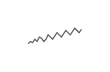
\begin{tikzpicture}[x=0.08em, y=0.08em, line width=0.4pt]
                \draw[FooterGray] (0,3) -- (1,4) -- (2,3.5) -- (3,5) -- (4,4) -- (5,6) -- (6,5.5) -- (7,4) -- (8,5) -- (9,7) -- (10,6) -- (11,5) -- (12,6.5) -- (13,8) -- (14,7) -- (15,6) -- (16,7.5) -- (17,9) -- (18,8) -- (19,7) -- (20,8.5) -- (21,10) -- (22,9) -- (23,8) -- (24,9.5);
            \end{tikzpicture}%
        }%
        \hskip0.5cm%
    }%
    \vskip6pt%
}

%=============================================================================
% PACKAGES
%=============================================================================
\usepackage[utf8]{inputenc}
\DeclareUnicodeCharacter{03B1}{\ensuremath{\alpha}}
\usepackage[T1]{fontenc}
\usepackage{amsmath, amssymb, amsthm}
\usepackage{mathtools}
\usepackage{bm}
\usepackage{tikz}
\usetikzlibrary{arrows.meta, positioning, shapes, calc, decorations.pathreplacing, shadings}
\usepackage{booktabs}
\usepackage{multirow}
\usepackage{array}
\usepackage{graphicx}
\usepackage{animate}
\usepackage{hyperref}
\usepackage{colortbl}
\usepackage{listings}
\lstset{language=Python, basicstyle=\ttfamily\scriptsize, keywordstyle=\color{MainBlue}\bfseries,
  commentstyle=\color{Forest}, stringstyle=\color{Crimson}, breaklines=true,
  frame=none, backgroundcolor=\color{VeryLightGray}, xleftmargin=2mm}
\hypersetup{colorlinks=true, linkcolor=MainBlue, urlcolor=MainBlue}
\graphicspath{{../../logos/}{../../charts/}{../../photos/}}
\usepackage{xcolor}
\hfuzz=2pt  % Suppress tiny overfull warnings (<2pt)
\vfuzz=2pt  % Suppress tiny vertical overfull warnings (<2pt)
% \mathrm in the sans-serif family of the slides (beamer resets \mathrm to the serif family at \begin{document};
% this hook runs after beamer's, so WN, Var, RMSE, ... in formulas match the surrounding text)
% Bold vectors and matrices in the same sans-serif family: \mathbf{A} in sans bold (beamer's own \mathbf came out in
% medium weight), and the bold upright Greek capitals of \boldsymbol / \bm (\bSigma, \bPhi, \boldsymbol{\Theta}) in
% cmss bold: bm.sty fixes its "boldoperators" font when it is loaded (serif cmbx), before beamer switches the
% operators to cmss, so it is reset here.
\AtBeginDocument{%
  \SetMathAlphabet{\mathrm}{normal}{\encodingdefault}{\sfdefault}{\mddefault}{n}%
  \SetMathAlphabet{\mathrm}{bold}{\encodingdefault}{\sfdefault}{bx}{n}%
  \SetMathAlphabet{\mathbf}{normal}{\encodingdefault}{\sfdefault}{bx}{n}%
  \SetMathAlphabet{\mathbf}{bold}{\encodingdefault}{\sfdefault}{bx}{n}%
  \SetSymbolFont{boldoperators}{normal}{OT1}{cmss}{bx}{n}%
  \SetSymbolFont{boldoperators}{bold}{OT1}{cmss}{bx}{n}}

%=============================================================================
% QUANTLET COMMANDS
%   \quantlet{<displayed name>}{<url>}       (generic, compatible with the older TSA decks)
%   \tsaquantlet{Ch_05}{TSA_ch5_garch}       -> https://github.com/danpele/Time-Series-Analysis/tree/main/Quantlets/Ch_05/TSA_ch5_garch
%   \qlurl{<folder>} is defined per chapter by the generator (Quantlets/Ch_NN/<folder>)
%=============================================================================
\newcommand{\tsarepo}{https://github.com/danpele/Time-Series-Analysis}
\newcommand{\tsaqlbase}{https://github.com/danpele/Time-Series-Analysis/tree/main/Quantlets}
\newcommand{\quantlet}[2]{%
    \hfill\href{#2}{%
        \raisebox{-0.15em}{
\includegraphics[height=0.7em]{ql_logo.png}}%
        \textcolor{MainBlue}{\tiny\ #1}%
    }%
}
\newcommand{\tsaquantlet}[2]{\quantlet{\detokenize{#2}}{\tsaqlbase/#1/#2}}

%=============================================================================
% NOTEBOOKS (Google Colab)
%   \colaburl{notebooks/EN/chapter5_seminar_notebook.ipynb} -> the Colab link of a file in the TSA repo
%   \nb: the chapter notebook (each seminar deck redefines it with \renewcommand)
%=============================================================================
\newcommand{\colaburl}[1]{https://colab.research.google.com/github/danpele/Time-Series-Analysis/blob/main/#1}
\newcommand{\nb}{https://colab.research.google.com/github/danpele/Time-Series-Analysis/tree/main/notebooks/EN}
\newcommand{\nbname}{notebooks/EN}

%=============================================================================
% SLIDE HELPERS (used by the generators; the same as in MFM)
%=============================================================================
% local font size for list bodies (the preamble forces \normalsize)
\newcommand{\itemsize}[1]{\setbeamertemplate{itemize/enumerate body begin}{#1}\setbeamertemplate{itemize/enumerate subbody begin}{#1}}
\newcommand{\intitle}[1]{{\hypersetup{urlcolor=white}#1}}   % white links inside coloured title bars
\newcommand{\imgcap}[1]{{\scriptsize #1}\\[0.5mm]}          % caption under a photo
\newcommand{\imgcredit}[2]{{\tiny\color{FooterGray}\href{#1}{#2}}}   % image credit: source URL, author/licence
\newcommand{\aiprompt}[1]{{\ttfamily\color{MainBlue}#1}}     % a prompt to an AI assistant

%=============================================================================
% SEMINARS: student version by default; the instructor wrapper *_solutions.tex sets \solutionstrue
%=============================================================================
\makeatletter\@ifundefined{ifsolutions}{\expandafter\newif\csname ifsolutions\endcsname}{}\makeatother
\newcommand{\solonly}[1]{\ifsolutions #1\fi}
\newcommand{\propsub}{\ifsolutions\else\framesubtitle{\ifdefined\tsalang Rezolvarea se discută la seminar\else Solution discussed in class\fi}\fi}

%=============================================================================
% APPENDIX AND CHAPTER LINKS (latex/appendix_links.py writes the calls; it also re-declares these
% macros before \begin{document}, so the decks compile with or without this preamble block)
%=============================================================================
\providecommand{\tsaapplink}[3]{\hypertarget{#2}{}\hyperlink{#1}{\beamergotobutton{#3}}}
\providecommand{\tsaappback}[2]{\begin{tikzpicture}[remember picture,overlay]\node[anchor=south east] at ([xshift=-3mm,yshift=7mm]current page.south east){\hyperlink{#1}{\beamerreturnbutton{#2}}};\end{tikzpicture}}
\providecommand{\tsachlink}[2]{\href{#1}{#2}}
\providecommand{\tsachlinkt}[2]{\href{#1}{\usebeamercolor[fg]{frametitle}#2}}

%=============================================================================
% QUANTINAR COMMAND: link către un curs Quantinar (subiecte avansate)
%=============================================================================
\newcommand{\quantinar}[2]{%
    \href{#2}{%
        \raisebox{-0.15em}{
\includegraphics[height=0.8em]{qr_logo.png}}%
        \textcolor{MainBlue}{\scriptsize\ #1}%
    }%
}

%=============================================================================
% CUSTOM TITLE PAGE
%=============================================================================
\defbeamertemplate*{title page}{hybrid}[1][]
{
    \vspace{0.2cm}
    % Logos row - top header (with clickable links)
    \begin{center}
        \href{https://www.ase.ro}{
\includegraphics[height=1.0cm]{ase_logo.png}}\hspace{0.3cm}%
        \href{https://theida.net}{
\includegraphics[height=1.0cm]{ida_logo.png}}\hspace{0.3cm}%
        \href{https://blockchain-research-center.com}{
\includegraphics[height=1.0cm]{brc_logo.png}}\hspace{0.3cm}%
        \href{https://www.ai4efin.ase.ro}{
\includegraphics[height=1.0cm]{ai4efin_logo.png}}\hspace{0.3cm}%
        \href{https://ipe.ro/new}{
\includegraphics[height=1.0cm]{acad_logo.png}}\hspace{0.3cm}%
        \href{https://www.digital-finance-msca.com}{
\includegraphics[height=1.0cm]{msca_logo.png}}%
    \end{center}

    \vspace{0.6cm}

    % Main title with Q logos on sides (with clickable links)
    \begin{center}
        \begin{minipage}{0.1\textwidth}
            \centering
            \href{https://quantlet.com}{
\includegraphics[height=1.1cm]{ql_logo.png}}
        \end{minipage}%
        \begin{minipage}{0.78\textwidth}
            \centering
            {\LARGE\bfseries\usebeamercolor[fg]{title}\inserttitle}

            \vspace{0.3cm}

            {\usebeamerfont{subtitle}\usebeamercolor[fg]{title}\insertsubtitle}
        \end{minipage}%
        \begin{minipage}{0.1\textwidth}
            \centering
            \href{https://quantinar.com}{
\includegraphics[height=1.1cm]{qr_logo.png}}
        \end{minipage}
    \end{center}

    \vspace{0.6cm}

    % Authors (left aligned)
    \hspace{0.5cm}{\usebeamerfont{author}\insertauthor}

    \vspace{0.3cm}

    % Institute/Affiliations (left aligned)
    \hspace{0.5cm}\begin{minipage}[t]{0.9\textwidth}
        \raggedright\small\insertinstitute
    \end{minipage}
}

%=============================================================================
% THEOREM ENVIRONMENTS
%=============================================================================
\theoremstyle{definition}
\setbeamertemplate{theorems}[numbered]
\ifdefined\tsalang
\newtheorem{defn}{Definiție}
\newtheorem{thm}{Teoremă}
\newtheorem{prop}{Propoziție}
\newtheorem{rmk}{Observație}
\else
\newtheorem{defn}{Definition}
\newtheorem{thm}{Theorem}
\newtheorem{prop}{Proposition}
\newtheorem{rmk}{Remark}
\fi

%=============================================================================
% CENTRED MINIPAGE (no extra vertical space)
%=============================================================================
\newenvironment{cminipage}[1]{%
    \par\noindent\hfill\begin{minipage}{#1}\ignorespaces
}{%
    \end{minipage}\hfill\null\par
}

%=============================================================================
% CUSTOM COMMANDS
%=============================================================================
\newcommand{\E}{\mathbb{E}}
\newcommand{\Var}{\text{Var}}
\newcommand{\Cov}{\text{Cov}}
\newcommand{\Corr}{\text{Corr}}
\newcommand{\R}{\mathbb{R}}
\newcommand{\N}{\mathbb{N}}
\newcommand{\Z}{\mathbb{Z}}
\newcommand{\B}{\mathbf{B}}
\newcommand{\imark}{\textcolor{MainBlue}{\textbullet}}
\newcommand{\RMSE}{\text{RMSE}}
\newcommand{\MAE}{\text{MAE}}
\newcommand{\MAPE}{\text{MAPE}}

% Boldface vector/matrix commands (VAR, VECM, state space; also used by the older TSA decks)
\newcommand{\bY}{\mathbf{Y}}
\newcommand{\bX}{\mathbf{X}}
\newcommand{\bA}{\mathbf{A}}
\newcommand{\bB}{\mathbf{B}}
\newcommand{\bepsilon}{\boldsymbol{\varepsilon}}
\newcommand{\bSigma}{\boldsymbol{\Sigma}}
\newcommand{\bPhi}{\boldsymbol{\Phi}}
\newcommand{\bGamma}{\boldsymbol{\Gamma}}
\newcommand{\bPi}{\boldsymbol{\Pi}}
\newcommand{\bc}{\mathbf{c}}
\newcommand{\balpha}{\boldsymbol{\alpha}}
\newcommand{\bbeta}{\boldsymbol{\beta}}
\newcommand{\bvarepsilon}{\boldsymbol{\varepsilon}}

% Legacy seminar marks (older TSA seminar decks)
\newcommand{\correct}{\textcolor{Forest}{\checkmark}}
\newcommand{\incorrect}{\textcolor{Crimson}{\texttimes}}
 se definește
%   \newcommand{\coursename}{Time Series Analysis}      (EN)
%   \newcommand{\coursename}{Serii de timp}       (RO)  și  \def\tsalang{ro}
% Fișierele .tex se află în EN/Courses, EN/Seminars, RO/Cursuri, RO/Seminarii (două niveluri sub rădăcină).
% Deck-urile sînt generate de latex/build_chapterN.py / build_seminarN.py (vezi latex/tsa_build.py).

\documentclass[9pt, aspectratio=169, t]{beamer}
\providecommand{\coursename}{Time Series Analysis}

% Ensure content fits on slides
\setbeamersize{text margin left=8mm, text margin right=8mm}
% Smaller institute font (title page)
\setbeamerfont{institute}{size=\footnotesize}

%=============================================================================
% THEME AND STYLE CONFIGURATION
%=============================================================================
\usetheme{default}
% Using default theme for clean header/footer control

% Color Palette (matching Redispatch PDF)
\definecolor{MainBlue}{RGB}{26, 58, 110}
\definecolor{AccentBlue}{RGB}{26, 58, 110}
\definecolor{IDAred}{RGB}{205, 0, 0}
\definecolor{DarkGray}{RGB}{51, 51, 51}
\definecolor{MediumGray}{RGB}{128, 128, 128}
\definecolor{LightGray}{RGB}{248, 248, 248}
\definecolor{VeryLightGray}{RGB}{235, 235, 235}
\definecolor{KeynoteGray}{RGB}{218, 218, 218}
\definecolor{SectionGray}{RGB}{120, 120, 120}
\definecolor{FooterGray}{RGB}{100, 100, 100}
\definecolor{Crimson}{RGB}{220, 53, 69}
\definecolor{Forest}{RGB}{46, 125, 50}
\definecolor{Amber}{RGB}{181, 133, 63}
\definecolor{Orange}{RGB}{230, 126, 34}
\definecolor{Purple}{RGB}{142, 68, 173}

% Gradient background (exact Keynote 315° gradient: white to RGB 218,218,218)
\setbeamertemplate{background}{%
    \begin{tikzpicture}[remember picture, overlay]
        \shade[shading=axis, shading angle=315,
        top color=white, bottom color=KeynoteGray]
        (current page.south west) rectangle (current page.north east);
    \end{tikzpicture}%
}
% Fallback solid color for compatibility
\setbeamercolor{background canvas}{bg=}

\setbeamercolor{palette primary}{bg=MainBlue, fg=white}
\setbeamercolor{palette secondary}{bg=MainBlue!85, fg=white}
\setbeamercolor{palette tertiary}{bg=MainBlue!70, fg=white}
\setbeamercolor{structure}{fg=MainBlue}
\setbeamercolor{title}{fg=IDAred}
\setbeamercolor{frametitle}{fg=IDAred, bg=}
\setbeamercolor{block title}{bg=MainBlue, fg=white}
\setbeamercolor{block body}{bg=VeryLightGray, fg=DarkGray}
\setbeamercolor{block title alerted}{bg=Crimson, fg=white}
\setbeamercolor{block body alerted}{bg=Crimson!8, fg=DarkGray}
\setbeamercolor{block title example}{bg=Forest, fg=white}
\setbeamercolor{block body example}{bg=Forest!8, fg=DarkGray}
\setbeamercolor{item}{fg=MainBlue}

% Footer colors (override Madrid theme blue)
\setbeamercolor{author in head/foot}{fg=FooterGray, bg=}
\setbeamercolor{title in head/foot}{fg=FooterGray, bg=}
\setbeamercolor{date in head/foot}{fg=FooterGray, bg=}
\setbeamercolor{section in head/foot}{fg=FooterGray, bg=}
\setbeamercolor{subsection in head/foot}{fg=FooterGray, bg=}

% Bullet styles (apply everywhere including blocks)
\setbeamertemplate{itemize item}{\color{MainBlue}$\boxdot$}
\setbeamertemplate{itemize subitem}{\color{MainBlue}$\blacktriangleright$}
\setbeamertemplate{itemize subsubitem}{\color{MainBlue}\tiny$\bullet$}
\setbeamertemplate{itemize/enumerate body begin}{\normalsize}
\setbeamertemplate{itemize/enumerate subbody begin}{\normalsize}

% Item spacing - compact style
\setlength{\leftmargini}{10pt}       % Level 1: minimal indent
\setlength{\leftmarginii}{10pt}      % Level 2: minimal additional indent
% Compact list spacing (zero extra space before/after lists in blocks)
\makeatletter
\def\@listi{\leftmargin\leftmargini \topsep 0pt \parsep 0pt \itemsep 0pt}
\def\@listii{\leftmargin\leftmarginii \topsep 0pt \parsep 0pt \itemsep 0pt}
\makeatother

\setbeamertemplate{navigation symbols}{}

%=============================================================================
% CUSTOM HEADLINE
%=============================================================================
\setbeamertemplate{headline}{%
    \vskip10pt%
    \hbox to \paperwidth{%
        \hskip0.5cm%
        {\small\color{FooterGray}\renewcommand{\hyperlink}[2]{##2}\insertsectionhead}%
        \hfill%
        \textcolor{FooterGray}{\small\insertframenumber}%
        \hskip0.5cm%
    }%
    \vskip4pt%
    {\color{FooterGray}\hrule height 0.4pt}%
}

%=============================================================================
% CUSTOM FOOTER
%=============================================================================
\usepackage{fontawesome5}

\setbeamertemplate{footline}{%
    {\color{FooterGray}\hrule height 0.4pt}%
    \vskip4pt%
    \hbox to \paperwidth{%
        \hskip0.5cm%
        \textcolor{FooterGray}{\small\coursename}%
        \hfill%
        \raisebox{-0.1em}{%
            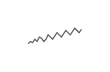
\begin{tikzpicture}[x=0.08em, y=0.08em, line width=0.4pt]
                \draw[FooterGray] (0,3) -- (1,4) -- (2,3.5) -- (3,5) -- (4,4) -- (5,6) -- (6,5.5) -- (7,4) -- (8,5) -- (9,7) -- (10,6) -- (11,5) -- (12,6.5) -- (13,8) -- (14,7) -- (15,6) -- (16,7.5) -- (17,9) -- (18,8) -- (19,7) -- (20,8.5) -- (21,10) -- (22,9) -- (23,8) -- (24,9.5);
            \end{tikzpicture}%
        }%
        \hskip0.5cm%
    }%
    \vskip6pt%
}

%=============================================================================
% PACKAGES
%=============================================================================
\usepackage[utf8]{inputenc}
\DeclareUnicodeCharacter{03B1}{\ensuremath{\alpha}}
\usepackage[T1]{fontenc}
\usepackage{amsmath, amssymb, amsthm}
\usepackage{mathtools}
\usepackage{bm}
\usepackage{tikz}
\usetikzlibrary{arrows.meta, positioning, shapes, calc, decorations.pathreplacing, shadings}
\usepackage{booktabs}
\usepackage{multirow}
\usepackage{array}
\usepackage{graphicx}
\usepackage{animate}
\usepackage{hyperref}
\usepackage{colortbl}
\usepackage{listings}
\lstset{language=Python, basicstyle=\ttfamily\scriptsize, keywordstyle=\color{MainBlue}\bfseries,
  commentstyle=\color{Forest}, stringstyle=\color{Crimson}, breaklines=true,
  frame=none, backgroundcolor=\color{VeryLightGray}, xleftmargin=2mm}
\hypersetup{colorlinks=true, linkcolor=MainBlue, urlcolor=MainBlue}
\graphicspath{{../../logos/}{../../charts/}{../../photos/}}
\usepackage{xcolor}
\hfuzz=2pt  % Suppress tiny overfull warnings (<2pt)
\vfuzz=2pt  % Suppress tiny vertical overfull warnings (<2pt)
% \mathrm in the sans-serif family of the slides (beamer resets \mathrm to the serif family at \begin{document};
% this hook runs after beamer's, so WN, Var, RMSE, ... in formulas match the surrounding text)
% Bold vectors and matrices in the same sans-serif family: \mathbf{A} in sans bold (beamer's own \mathbf came out in
% medium weight), and the bold upright Greek capitals of \boldsymbol / \bm (\bSigma, \bPhi, \boldsymbol{\Theta}) in
% cmss bold: bm.sty fixes its "boldoperators" font when it is loaded (serif cmbx), before beamer switches the
% operators to cmss, so it is reset here.
\AtBeginDocument{%
  \SetMathAlphabet{\mathrm}{normal}{\encodingdefault}{\sfdefault}{\mddefault}{n}%
  \SetMathAlphabet{\mathrm}{bold}{\encodingdefault}{\sfdefault}{bx}{n}%
  \SetMathAlphabet{\mathbf}{normal}{\encodingdefault}{\sfdefault}{bx}{n}%
  \SetMathAlphabet{\mathbf}{bold}{\encodingdefault}{\sfdefault}{bx}{n}%
  \SetSymbolFont{boldoperators}{normal}{OT1}{cmss}{bx}{n}%
  \SetSymbolFont{boldoperators}{bold}{OT1}{cmss}{bx}{n}}

%=============================================================================
% QUANTLET COMMANDS
%   \quantlet{<displayed name>}{<url>}       (generic, compatible with the older TSA decks)
%   \tsaquantlet{Ch_05}{TSA_ch5_garch}       -> https://github.com/danpele/Time-Series-Analysis/tree/main/Quantlets/Ch_05/TSA_ch5_garch
%   \qlurl{<folder>} is defined per chapter by the generator (Quantlets/Ch_NN/<folder>)
%=============================================================================
\newcommand{\tsarepo}{https://github.com/danpele/Time-Series-Analysis}
\newcommand{\tsaqlbase}{https://github.com/danpele/Time-Series-Analysis/tree/main/Quantlets}
\newcommand{\quantlet}[2]{%
    \hfill\href{#2}{%
        \raisebox{-0.15em}{
\includegraphics[height=0.7em]{ql_logo.png}}%
        \textcolor{MainBlue}{\tiny\ #1}%
    }%
}
\newcommand{\tsaquantlet}[2]{\quantlet{\detokenize{#2}}{\tsaqlbase/#1/#2}}

%=============================================================================
% NOTEBOOKS (Google Colab)
%   \colaburl{notebooks/EN/chapter5_seminar_notebook.ipynb} -> the Colab link of a file in the TSA repo
%   \nb: the chapter notebook (each seminar deck redefines it with \renewcommand)
%=============================================================================
\newcommand{\colaburl}[1]{https://colab.research.google.com/github/danpele/Time-Series-Analysis/blob/main/#1}
\newcommand{\nb}{https://colab.research.google.com/github/danpele/Time-Series-Analysis/tree/main/notebooks/EN}
\newcommand{\nbname}{notebooks/EN}

%=============================================================================
% SLIDE HELPERS (used by the generators; the same as in MFM)
%=============================================================================
% local font size for list bodies (the preamble forces \normalsize)
\newcommand{\itemsize}[1]{\setbeamertemplate{itemize/enumerate body begin}{#1}\setbeamertemplate{itemize/enumerate subbody begin}{#1}}
\newcommand{\intitle}[1]{{\hypersetup{urlcolor=white}#1}}   % white links inside coloured title bars
\newcommand{\imgcap}[1]{{\scriptsize #1}\\[0.5mm]}          % caption under a photo
\newcommand{\imgcredit}[2]{{\tiny\color{FooterGray}\href{#1}{#2}}}   % image credit: source URL, author/licence
\newcommand{\aiprompt}[1]{{\ttfamily\color{MainBlue}#1}}     % a prompt to an AI assistant

%=============================================================================
% SEMINARS: student version by default; the instructor wrapper *_solutions.tex sets \solutionstrue
%=============================================================================
\makeatletter\@ifundefined{ifsolutions}{\expandafter\newif\csname ifsolutions\endcsname}{}\makeatother
\newcommand{\solonly}[1]{\ifsolutions #1\fi}
\newcommand{\propsub}{\ifsolutions\else\framesubtitle{\ifdefined\tsalang Rezolvarea se discută la seminar\else Solution discussed in class\fi}\fi}

%=============================================================================
% APPENDIX AND CHAPTER LINKS (latex/appendix_links.py writes the calls; it also re-declares these
% macros before \begin{document}, so the decks compile with or without this preamble block)
%=============================================================================
\providecommand{\tsaapplink}[3]{\hypertarget{#2}{}\hyperlink{#1}{\beamergotobutton{#3}}}
\providecommand{\tsaappback}[2]{\begin{tikzpicture}[remember picture,overlay]\node[anchor=south east] at ([xshift=-3mm,yshift=7mm]current page.south east){\hyperlink{#1}{\beamerreturnbutton{#2}}};\end{tikzpicture}}
\providecommand{\tsachlink}[2]{\href{#1}{#2}}
\providecommand{\tsachlinkt}[2]{\href{#1}{\usebeamercolor[fg]{frametitle}#2}}

%=============================================================================
% QUANTINAR COMMAND: link către un curs Quantinar (subiecte avansate)
%=============================================================================
\newcommand{\quantinar}[2]{%
    \href{#2}{%
        \raisebox{-0.15em}{
\includegraphics[height=0.8em]{qr_logo.png}}%
        \textcolor{MainBlue}{\scriptsize\ #1}%
    }%
}

%=============================================================================
% CUSTOM TITLE PAGE
%=============================================================================
\defbeamertemplate*{title page}{hybrid}[1][]
{
    \vspace{0.2cm}
    % Logos row - top header (with clickable links)
    \begin{center}
        \href{https://www.ase.ro}{
\includegraphics[height=1.0cm]{ase_logo.png}}\hspace{0.3cm}%
        \href{https://theida.net}{
\includegraphics[height=1.0cm]{ida_logo.png}}\hspace{0.3cm}%
        \href{https://blockchain-research-center.com}{
\includegraphics[height=1.0cm]{brc_logo.png}}\hspace{0.3cm}%
        \href{https://www.ai4efin.ase.ro}{
\includegraphics[height=1.0cm]{ai4efin_logo.png}}\hspace{0.3cm}%
        \href{https://ipe.ro/new}{
\includegraphics[height=1.0cm]{acad_logo.png}}\hspace{0.3cm}%
        \href{https://www.digital-finance-msca.com}{
\includegraphics[height=1.0cm]{msca_logo.png}}%
    \end{center}

    \vspace{0.6cm}

    % Main title with Q logos on sides (with clickable links)
    \begin{center}
        \begin{minipage}{0.1\textwidth}
            \centering
            \href{https://quantlet.com}{
\includegraphics[height=1.1cm]{ql_logo.png}}
        \end{minipage}%
        \begin{minipage}{0.78\textwidth}
            \centering
            {\LARGE\bfseries\usebeamercolor[fg]{title}\inserttitle}

            \vspace{0.3cm}

            {\usebeamerfont{subtitle}\usebeamercolor[fg]{title}\insertsubtitle}
        \end{minipage}%
        \begin{minipage}{0.1\textwidth}
            \centering
            \href{https://quantinar.com}{
\includegraphics[height=1.1cm]{qr_logo.png}}
        \end{minipage}
    \end{center}

    \vspace{0.6cm}

    % Authors (left aligned)
    \hspace{0.5cm}{\usebeamerfont{author}\insertauthor}

    \vspace{0.3cm}

    % Institute/Affiliations (left aligned)
    \hspace{0.5cm}\begin{minipage}[t]{0.9\textwidth}
        \raggedright\small\insertinstitute
    \end{minipage}
}

%=============================================================================
% THEOREM ENVIRONMENTS
%=============================================================================
\theoremstyle{definition}
\setbeamertemplate{theorems}[numbered]
\ifdefined\tsalang
\newtheorem{defn}{Definiție}
\newtheorem{thm}{Teoremă}
\newtheorem{prop}{Propoziție}
\newtheorem{rmk}{Observație}
\else
\newtheorem{defn}{Definition}
\newtheorem{thm}{Theorem}
\newtheorem{prop}{Proposition}
\newtheorem{rmk}{Remark}
\fi

%=============================================================================
% CENTRED MINIPAGE (no extra vertical space)
%=============================================================================
\newenvironment{cminipage}[1]{%
    \par\noindent\hfill\begin{minipage}{#1}\ignorespaces
}{%
    \end{minipage}\hfill\null\par
}

%=============================================================================
% CUSTOM COMMANDS
%=============================================================================
\newcommand{\E}{\mathbb{E}}
\newcommand{\Var}{\text{Var}}
\newcommand{\Cov}{\text{Cov}}
\newcommand{\Corr}{\text{Corr}}
\newcommand{\R}{\mathbb{R}}
\newcommand{\N}{\mathbb{N}}
\newcommand{\Z}{\mathbb{Z}}
\newcommand{\B}{\mathbf{B}}
\newcommand{\imark}{\textcolor{MainBlue}{\textbullet}}
\newcommand{\RMSE}{\text{RMSE}}
\newcommand{\MAE}{\text{MAE}}
\newcommand{\MAPE}{\text{MAPE}}

% Boldface vector/matrix commands (VAR, VECM, state space; also used by the older TSA decks)
\newcommand{\bY}{\mathbf{Y}}
\newcommand{\bX}{\mathbf{X}}
\newcommand{\bA}{\mathbf{A}}
\newcommand{\bB}{\mathbf{B}}
\newcommand{\bepsilon}{\boldsymbol{\varepsilon}}
\newcommand{\bSigma}{\boldsymbol{\Sigma}}
\newcommand{\bPhi}{\boldsymbol{\Phi}}
\newcommand{\bGamma}{\boldsymbol{\Gamma}}
\newcommand{\bPi}{\boldsymbol{\Pi}}
\newcommand{\bc}{\mathbf{c}}
\newcommand{\balpha}{\boldsymbol{\alpha}}
\newcommand{\bbeta}{\boldsymbol{\beta}}
\newcommand{\bvarepsilon}{\boldsymbol{\varepsilon}}

% Legacy seminar marks (older TSA seminar decks)
\newcommand{\correct}{\textcolor{Forest}{\checkmark}}
\newcommand{\incorrect}{\textcolor{Crimson}{\texttimes}}
 se definește
%   \newcommand{\coursename}{Time Series Analysis}      (EN)
%   \newcommand{\coursename}{Serii de timp}       (RO)  și  \def\tsalang{ro}
% Fișierele .tex se află în EN/Courses, EN/Seminars, RO/Cursuri, RO/Seminarii (două niveluri sub rădăcină).
% Deck-urile sînt generate de latex/build_chapterN.py / build_seminarN.py (vezi latex/tsa_build.py).

\documentclass[9pt, aspectratio=169, t]{beamer}
\providecommand{\coursename}{Time Series Analysis}

% Ensure content fits on slides
\setbeamersize{text margin left=8mm, text margin right=8mm}
% Smaller institute font (title page)
\setbeamerfont{institute}{size=\footnotesize}

%=============================================================================
% THEME AND STYLE CONFIGURATION
%=============================================================================
\usetheme{default}
% Using default theme for clean header/footer control

% Color Palette (matching Redispatch PDF)
\definecolor{MainBlue}{RGB}{26, 58, 110}
\definecolor{AccentBlue}{RGB}{26, 58, 110}
\definecolor{IDAred}{RGB}{205, 0, 0}
\definecolor{DarkGray}{RGB}{51, 51, 51}
\definecolor{MediumGray}{RGB}{128, 128, 128}
\definecolor{LightGray}{RGB}{248, 248, 248}
\definecolor{VeryLightGray}{RGB}{235, 235, 235}
\definecolor{KeynoteGray}{RGB}{218, 218, 218}
\definecolor{SectionGray}{RGB}{120, 120, 120}
\definecolor{FooterGray}{RGB}{100, 100, 100}
\definecolor{Crimson}{RGB}{220, 53, 69}
\definecolor{Forest}{RGB}{46, 125, 50}
\definecolor{Amber}{RGB}{181, 133, 63}
\definecolor{Orange}{RGB}{230, 126, 34}
\definecolor{Purple}{RGB}{142, 68, 173}

% Gradient background (exact Keynote 315° gradient: white to RGB 218,218,218)
\setbeamertemplate{background}{%
    \begin{tikzpicture}[remember picture, overlay]
        \shade[shading=axis, shading angle=315,
        top color=white, bottom color=KeynoteGray]
        (current page.south west) rectangle (current page.north east);
    \end{tikzpicture}%
}
% Fallback solid color for compatibility
\setbeamercolor{background canvas}{bg=}

\setbeamercolor{palette primary}{bg=MainBlue, fg=white}
\setbeamercolor{palette secondary}{bg=MainBlue!85, fg=white}
\setbeamercolor{palette tertiary}{bg=MainBlue!70, fg=white}
\setbeamercolor{structure}{fg=MainBlue}
\setbeamercolor{title}{fg=IDAred}
\setbeamercolor{frametitle}{fg=IDAred, bg=}
\setbeamercolor{block title}{bg=MainBlue, fg=white}
\setbeamercolor{block body}{bg=VeryLightGray, fg=DarkGray}
\setbeamercolor{block title alerted}{bg=Crimson, fg=white}
\setbeamercolor{block body alerted}{bg=Crimson!8, fg=DarkGray}
\setbeamercolor{block title example}{bg=Forest, fg=white}
\setbeamercolor{block body example}{bg=Forest!8, fg=DarkGray}
\setbeamercolor{item}{fg=MainBlue}

% Footer colors (override Madrid theme blue)
\setbeamercolor{author in head/foot}{fg=FooterGray, bg=}
\setbeamercolor{title in head/foot}{fg=FooterGray, bg=}
\setbeamercolor{date in head/foot}{fg=FooterGray, bg=}
\setbeamercolor{section in head/foot}{fg=FooterGray, bg=}
\setbeamercolor{subsection in head/foot}{fg=FooterGray, bg=}

% Bullet styles (apply everywhere including blocks)
\setbeamertemplate{itemize item}{\color{MainBlue}$\boxdot$}
\setbeamertemplate{itemize subitem}{\color{MainBlue}$\blacktriangleright$}
\setbeamertemplate{itemize subsubitem}{\color{MainBlue}\tiny$\bullet$}
\setbeamertemplate{itemize/enumerate body begin}{\normalsize}
\setbeamertemplate{itemize/enumerate subbody begin}{\normalsize}

% Item spacing - compact style
\setlength{\leftmargini}{10pt}       % Level 1: minimal indent
\setlength{\leftmarginii}{10pt}      % Level 2: minimal additional indent
% Compact list spacing (zero extra space before/after lists in blocks)
\makeatletter
\def\@listi{\leftmargin\leftmargini \topsep 0pt \parsep 0pt \itemsep 0pt}
\def\@listii{\leftmargin\leftmarginii \topsep 0pt \parsep 0pt \itemsep 0pt}
\makeatother

\setbeamertemplate{navigation symbols}{}

%=============================================================================
% CUSTOM HEADLINE
%=============================================================================
\setbeamertemplate{headline}{%
    \vskip10pt%
    \hbox to \paperwidth{%
        \hskip0.5cm%
        {\small\color{FooterGray}\renewcommand{\hyperlink}[2]{##2}\insertsectionhead}%
        \hfill%
        \textcolor{FooterGray}{\small\insertframenumber}%
        \hskip0.5cm%
    }%
    \vskip4pt%
    {\color{FooterGray}\hrule height 0.4pt}%
}

%=============================================================================
% CUSTOM FOOTER
%=============================================================================
\usepackage{fontawesome5}

\setbeamertemplate{footline}{%
    {\color{FooterGray}\hrule height 0.4pt}%
    \vskip4pt%
    \hbox to \paperwidth{%
        \hskip0.5cm%
        \textcolor{FooterGray}{\small\coursename}%
        \hfill%
        \raisebox{-0.1em}{%
            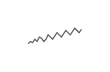
\begin{tikzpicture}[x=0.08em, y=0.08em, line width=0.4pt]
                \draw[FooterGray] (0,3) -- (1,4) -- (2,3.5) -- (3,5) -- (4,4) -- (5,6) -- (6,5.5) -- (7,4) -- (8,5) -- (9,7) -- (10,6) -- (11,5) -- (12,6.5) -- (13,8) -- (14,7) -- (15,6) -- (16,7.5) -- (17,9) -- (18,8) -- (19,7) -- (20,8.5) -- (21,10) -- (22,9) -- (23,8) -- (24,9.5);
            \end{tikzpicture}%
        }%
        \hskip0.5cm%
    }%
    \vskip6pt%
}

%=============================================================================
% PACKAGES
%=============================================================================
\usepackage[utf8]{inputenc}
\DeclareUnicodeCharacter{03B1}{\ensuremath{\alpha}}
\usepackage[T1]{fontenc}
\usepackage{amsmath, amssymb, amsthm}
\usepackage{mathtools}
\usepackage{bm}
\usepackage{tikz}
\usetikzlibrary{arrows.meta, positioning, shapes, calc, decorations.pathreplacing, shadings}
\usepackage{booktabs}
\usepackage{multirow}
\usepackage{array}
\usepackage{graphicx}
\usepackage{animate}
\usepackage{hyperref}
\usepackage{colortbl}
\usepackage{listings}
\lstset{language=Python, basicstyle=\ttfamily\scriptsize, keywordstyle=\color{MainBlue}\bfseries,
  commentstyle=\color{Forest}, stringstyle=\color{Crimson}, breaklines=true,
  frame=none, backgroundcolor=\color{VeryLightGray}, xleftmargin=2mm}
\hypersetup{colorlinks=true, linkcolor=MainBlue, urlcolor=MainBlue}
\graphicspath{{../../logos/}{../../charts/}{../../photos/}}
\usepackage{xcolor}
\hfuzz=2pt  % Suppress tiny overfull warnings (<2pt)
\vfuzz=2pt  % Suppress tiny vertical overfull warnings (<2pt)
% \mathrm in the sans-serif family of the slides (beamer resets \mathrm to the serif family at \begin{document};
% this hook runs after beamer's, so WN, Var, RMSE, ... in formulas match the surrounding text)
% Bold vectors and matrices in the same sans-serif family: \mathbf{A} in sans bold (beamer's own \mathbf came out in
% medium weight), and the bold upright Greek capitals of \boldsymbol / \bm (\bSigma, \bPhi, \boldsymbol{\Theta}) in
% cmss bold: bm.sty fixes its "boldoperators" font when it is loaded (serif cmbx), before beamer switches the
% operators to cmss, so it is reset here.
\AtBeginDocument{%
  \SetMathAlphabet{\mathrm}{normal}{\encodingdefault}{\sfdefault}{\mddefault}{n}%
  \SetMathAlphabet{\mathrm}{bold}{\encodingdefault}{\sfdefault}{bx}{n}%
  \SetMathAlphabet{\mathbf}{normal}{\encodingdefault}{\sfdefault}{bx}{n}%
  \SetMathAlphabet{\mathbf}{bold}{\encodingdefault}{\sfdefault}{bx}{n}%
  \SetSymbolFont{boldoperators}{normal}{OT1}{cmss}{bx}{n}%
  \SetSymbolFont{boldoperators}{bold}{OT1}{cmss}{bx}{n}}

%=============================================================================
% QUANTLET COMMANDS
%   \quantlet{<displayed name>}{<url>}       (generic, compatible with the older TSA decks)
%   \tsaquantlet{Ch_05}{TSA_ch5_garch}       -> https://github.com/danpele/Time-Series-Analysis/tree/main/Quantlets/Ch_05/TSA_ch5_garch
%   \qlurl{<folder>} is defined per chapter by the generator (Quantlets/Ch_NN/<folder>)
%=============================================================================
\newcommand{\tsarepo}{https://github.com/danpele/Time-Series-Analysis}
\newcommand{\tsaqlbase}{https://github.com/danpele/Time-Series-Analysis/tree/main/Quantlets}
\newcommand{\quantlet}[2]{%
    \hfill\href{#2}{%
        \raisebox{-0.15em}{
\includegraphics[height=0.7em]{ql_logo.png}}%
        \textcolor{MainBlue}{\tiny\ #1}%
    }%
}
\newcommand{\tsaquantlet}[2]{\quantlet{\detokenize{#2}}{\tsaqlbase/#1/#2}}

%=============================================================================
% NOTEBOOKS (Google Colab)
%   \colaburl{notebooks/EN/chapter5_seminar_notebook.ipynb} -> the Colab link of a file in the TSA repo
%   \nb: the chapter notebook (each seminar deck redefines it with \renewcommand)
%=============================================================================
\newcommand{\colaburl}[1]{https://colab.research.google.com/github/danpele/Time-Series-Analysis/blob/main/#1}
\newcommand{\nb}{https://colab.research.google.com/github/danpele/Time-Series-Analysis/tree/main/notebooks/EN}
\newcommand{\nbname}{notebooks/EN}

%=============================================================================
% SLIDE HELPERS (used by the generators; the same as in MFM)
%=============================================================================
% local font size for list bodies (the preamble forces \normalsize)
\newcommand{\itemsize}[1]{\setbeamertemplate{itemize/enumerate body begin}{#1}\setbeamertemplate{itemize/enumerate subbody begin}{#1}}
\newcommand{\intitle}[1]{{\hypersetup{urlcolor=white}#1}}   % white links inside coloured title bars
\newcommand{\imgcap}[1]{{\scriptsize #1}\\[0.5mm]}          % caption under a photo
\newcommand{\imgcredit}[2]{{\tiny\color{FooterGray}\href{#1}{#2}}}   % image credit: source URL, author/licence
\newcommand{\aiprompt}[1]{{\ttfamily\color{MainBlue}#1}}     % a prompt to an AI assistant

%=============================================================================
% SEMINARS: student version by default; the instructor wrapper *_solutions.tex sets \solutionstrue
%=============================================================================
\makeatletter\@ifundefined{ifsolutions}{\expandafter\newif\csname ifsolutions\endcsname}{}\makeatother
\newcommand{\solonly}[1]{\ifsolutions #1\fi}
\newcommand{\propsub}{\ifsolutions\else\framesubtitle{\ifdefined\tsalang Rezolvarea se discută la seminar\else Solution discussed in class\fi}\fi}

%=============================================================================
% APPENDIX AND CHAPTER LINKS (latex/appendix_links.py writes the calls; it also re-declares these
% macros before \begin{document}, so the decks compile with or without this preamble block)
%=============================================================================
\providecommand{\tsaapplink}[3]{\hypertarget{#2}{}\hyperlink{#1}{\beamergotobutton{#3}}}
\providecommand{\tsaappback}[2]{\begin{tikzpicture}[remember picture,overlay]\node[anchor=south east] at ([xshift=-3mm,yshift=7mm]current page.south east){\hyperlink{#1}{\beamerreturnbutton{#2}}};\end{tikzpicture}}
\providecommand{\tsachlink}[2]{\href{#1}{#2}}
\providecommand{\tsachlinkt}[2]{\href{#1}{\usebeamercolor[fg]{frametitle}#2}}

%=============================================================================
% QUANTINAR COMMAND: link către un curs Quantinar (subiecte avansate)
%=============================================================================
\newcommand{\quantinar}[2]{%
    \href{#2}{%
        \raisebox{-0.15em}{
\includegraphics[height=0.8em]{qr_logo.png}}%
        \textcolor{MainBlue}{\scriptsize\ #1}%
    }%
}

%=============================================================================
% CUSTOM TITLE PAGE
%=============================================================================
\defbeamertemplate*{title page}{hybrid}[1][]
{
    \vspace{0.2cm}
    % Logos row - top header (with clickable links)
    \begin{center}
        \href{https://www.ase.ro}{
\includegraphics[height=1.0cm]{ase_logo.png}}\hspace{0.3cm}%
        \href{https://theida.net}{
\includegraphics[height=1.0cm]{ida_logo.png}}\hspace{0.3cm}%
        \href{https://blockchain-research-center.com}{
\includegraphics[height=1.0cm]{brc_logo.png}}\hspace{0.3cm}%
        \href{https://www.ai4efin.ase.ro}{
\includegraphics[height=1.0cm]{ai4efin_logo.png}}\hspace{0.3cm}%
        \href{https://ipe.ro/new}{
\includegraphics[height=1.0cm]{acad_logo.png}}\hspace{0.3cm}%
        \href{https://www.digital-finance-msca.com}{
\includegraphics[height=1.0cm]{msca_logo.png}}%
    \end{center}

    \vspace{0.6cm}

    % Main title with Q logos on sides (with clickable links)
    \begin{center}
        \begin{minipage}{0.1\textwidth}
            \centering
            \href{https://quantlet.com}{
\includegraphics[height=1.1cm]{ql_logo.png}}
        \end{minipage}%
        \begin{minipage}{0.78\textwidth}
            \centering
            {\LARGE\bfseries\usebeamercolor[fg]{title}\inserttitle}

            \vspace{0.3cm}

            {\usebeamerfont{subtitle}\usebeamercolor[fg]{title}\insertsubtitle}
        \end{minipage}%
        \begin{minipage}{0.1\textwidth}
            \centering
            \href{https://quantinar.com}{
\includegraphics[height=1.1cm]{qr_logo.png}}
        \end{minipage}
    \end{center}

    \vspace{0.6cm}

    % Authors (left aligned)
    \hspace{0.5cm}{\usebeamerfont{author}\insertauthor}

    \vspace{0.3cm}

    % Institute/Affiliations (left aligned)
    \hspace{0.5cm}\begin{minipage}[t]{0.9\textwidth}
        \raggedright\small\insertinstitute
    \end{minipage}
}

%=============================================================================
% THEOREM ENVIRONMENTS
%=============================================================================
\theoremstyle{definition}
\setbeamertemplate{theorems}[numbered]
\ifdefined\tsalang
\newtheorem{defn}{Definiție}
\newtheorem{thm}{Teoremă}
\newtheorem{prop}{Propoziție}
\newtheorem{rmk}{Observație}
\else
\newtheorem{defn}{Definition}
\newtheorem{thm}{Theorem}
\newtheorem{prop}{Proposition}
\newtheorem{rmk}{Remark}
\fi

%=============================================================================
% CENTRED MINIPAGE (no extra vertical space)
%=============================================================================
\newenvironment{cminipage}[1]{%
    \par\noindent\hfill\begin{minipage}{#1}\ignorespaces
}{%
    \end{minipage}\hfill\null\par
}

%=============================================================================
% CUSTOM COMMANDS
%=============================================================================
\newcommand{\E}{\mathbb{E}}
\newcommand{\Var}{\text{Var}}
\newcommand{\Cov}{\text{Cov}}
\newcommand{\Corr}{\text{Corr}}
\newcommand{\R}{\mathbb{R}}
\newcommand{\N}{\mathbb{N}}
\newcommand{\Z}{\mathbb{Z}}
\newcommand{\B}{\mathbf{B}}
\newcommand{\imark}{\textcolor{MainBlue}{\textbullet}}
\newcommand{\RMSE}{\text{RMSE}}
\newcommand{\MAE}{\text{MAE}}
\newcommand{\MAPE}{\text{MAPE}}

% Boldface vector/matrix commands (VAR, VECM, state space; also used by the older TSA decks)
\newcommand{\bY}{\mathbf{Y}}
\newcommand{\bX}{\mathbf{X}}
\newcommand{\bA}{\mathbf{A}}
\newcommand{\bB}{\mathbf{B}}
\newcommand{\bepsilon}{\boldsymbol{\varepsilon}}
\newcommand{\bSigma}{\boldsymbol{\Sigma}}
\newcommand{\bPhi}{\boldsymbol{\Phi}}
\newcommand{\bGamma}{\boldsymbol{\Gamma}}
\newcommand{\bPi}{\boldsymbol{\Pi}}
\newcommand{\bc}{\mathbf{c}}
\newcommand{\balpha}{\boldsymbol{\alpha}}
\newcommand{\bbeta}{\boldsymbol{\beta}}
\newcommand{\bvarepsilon}{\boldsymbol{\varepsilon}}

% Legacy seminar marks (older TSA seminar decks)
\newcommand{\correct}{\textcolor{Forest}{\checkmark}}
\newcommand{\incorrect}{\textcolor{Crimson}{\texttimes}}


\newcommand{\qlurl}[1]{https://github.com/danpele/Time-Series-Analysis/tree/main/Quantlets/Ch_04/#1}

% Clickable citations (DOIs verified via Crossref)
\newcommand{\refHP}{\href{https://doi.org/10.1007/978-3-031-13584-2}{Huang and Petukhina (2022)}}
\newcommand{\refFPP}{\href{https://otexts.com/fpp3/}{Hyndman and Athanasopoulos (2021)}}
\newcommand{\refFPPsar}{\href{https://otexts.com/fpp3/seasonal-arima.html}{FPP3, Section 9.9}}
\newcommand{\refFPPcomplex}{\href{https://otexts.com/fpp3/complexseasonality.html}{FPP3, Section 12.1}}
\newcommand{\refFPPcv}{\href{https://otexts.com/fpp3/tscv.html}{FPP3, Section 5.10}}
\newcommand{\refFPPdhr}{\href{https://otexts.com/fpp3/dhr.html}{FPP3, Section 10.5}}
\newcommand{\refBD}{\href{https://doi.org/10.1007/978-3-319-29854-2}{Brockwell and Davis (2016)}}
\newcommand{\refBJ}{\href{https://doi.org/10.1002/9781118619193}{Box, Jenkins and Reinsel (2008)}}
\newcommand{\refBoxCox}{\href{https://doi.org/10.1111/j.2517-6161.1964.tb00553.x}{Box and Cox (1964)}}
\newcommand{\refHEGY}{\href{https://doi.org/10.1016/0304-4076(90)90080-D}{Hylleberg, Engle, Granger and Yoo (1990)}}
\newcommand{\refCH}{\href{https://doi.org/10.1080/07350015.1995.10524598}{Canova and Hansen (1995)}}
\newcommand{\refOCSB}{\href{https://doi.org/10.1111/j.1468-0084.1988.mp50004002.x}{Osborn, Chui, Smith and Birchenhall (1988)}}
\newcommand{\refFindley}{\href{https://doi.org/10.1080/07350015.1998.10524743}{Findley et al. (1998)}}
\newcommand{\refLadiray}{\href{https://doi.org/10.1007/978-1-4613-0175-2}{Ladiray and Quenneville (2001)}}
\newcommand{\refDagum}{\href{https://doi.org/10.1007/978-3-319-31822-6}{Dagum and Bianconcini (2016)}}
\newcommand{\refESS}{\href{https://ec.europa.eu/eurostat/web/products-manuals-and-guidelines/w/ks-gq-24-012}{Eurostat (2024)}}
\newcommand{\refMSTL}{\href{https://doi.org/10.1504/ijor.2025.143957}{Bandara, Hyndman and Bergmeir (2025)}}
\newcommand{\refTBATS}{\href{https://doi.org/10.1198/jasa.2011.tm09771}{De Livera, Hyndman and Snyder (2011)}}
\newcommand{\refProphet}{\href{https://doi.org/10.1080/00031305.2017.1380080}{Taylor and Letham (2018)}}
\newcommand{\refDM}{\href{https://doi.org/10.1080/07350015.1995.10524599}{Diebold and Mariano (1995)}}
\newcommand{\refHLN}{\href{https://doi.org/10.1016/S0169-2070(96)00719-4}{Harvey, Leybourne and Newbold (1997)}}
\newcommand{\refTashman}{\href{https://doi.org/10.1016/S0169-2070(00)00065-0}{Tashman (2000)}}
\newcommand{\refBHK}{\href{https://doi.org/10.1016/j.csda.2017.11.003}{Bergmeir, Hyndman and Koo (2018)}}
\newcommand{\refHKo}{\href{https://doi.org/10.1016/j.ijforecast.2006.03.001}{Hyndman and Koehler (2006)}}
\newcommand{\refHK}{\href{https://doi.org/10.18637/jss.v027.i03}{Hyndman and Khandakar (2008)}}
\newcommand{\refBG}{\href{https://doi.org/10.1057/jors.1969.103}{Bates and Granger (1969)}}
\newcommand{\refSW}{\href{https://doi.org/10.1002/for.928}{Stock and Watson (2004)}}
\newcommand{\refSmithWallis}{\href{https://doi.org/10.1111/j.1468-0084.2008.00541.x}{Smith and Wallis (2009)}}
\newcommand{\refWangComb}{\href{https://doi.org/10.1016/j.ijforecast.2022.11.005}{Wang et al. (2023)}}
\newcommand{\refMFour}{\href{https://doi.org/10.1016/j.ijforecast.2019.04.014}{Makridakis, Spiliotis and Assimakopoulos (2020)}}
\newcommand{\refGEF}{\href{https://doi.org/10.1016/j.ijforecast.2016.02.001}{Hong et al. (2016)}}
\newcommand{\refPetro}{\href{https://doi.org/10.1016/j.ijforecast.2021.11.001}{Petropoulos et al. (2022)}}
\newcommand{\refLB}{\href{https://doi.org/10.1093/biomet/65.2.297}{Ljung and Box (1978)}}

\title[Time Series Analysis]{Time Series Analysis}
\subtitle{Chapter 4: Seasonality and forecasting: SARIMA, TBATS, Prophet}
\author[D.T. Pele]{Daniel Traian PELE}
\institute{Bucharest University of Economic Studies\\
IDA Institute Digital Assets\\
Blockchain Research Center\\
AI4EFin Artificial Intelligence for Energy Finance\\
Romanian Academy, Institute for Economic Forecasting\\
MSCA Digital Finance}
\date{}

%=============================================================================
\providecommand{\tsaapplink}[3]{\hypertarget{#2}{}\hyperlink{#1}{\beamergotobutton{#3}}}  % APPLINKS-MACROS
\providecommand{\tsaappback}[2]{\begin{tikzpicture}[remember picture,overlay]\node[anchor=south east] at ([xshift=-3mm,yshift=7mm]current page.south east){\hyperlink{#1}{\beamerreturnbutton{#2}}};\end{tikzpicture}}  % APPLINKS-MACROS
\providecommand{\tsachlink}[2]{\href{#1}{#2}}  % APPLINKS-MACROS
\providecommand{\tsachlinkt}[2]{\href{#1}{\usebeamercolor[fg]{frametitle}#2}}  % APPLINKS-MACROS
\begin{document}
%=============================================================================

{
\setbeamertemplate{headline}{}
\setbeamertemplate{footline}{}
\begin{frame}[noframenumbering]
    \titlepage
\end{frame}
}
% BEGIN-ACRONYMS (generat de latex/acronyms.py; nu editati manual)
\begin{frame}{Acronyms used in this material (1/2)}
\setbeamertemplate{itemize/enumerate body begin}{\tiny}
\begin{columns}[T]
\begin{column}{0.49\textwidth}
\begin{itemize}\setlength{\itemsep}{0pt}
    \item \textbf{ACF}: Autocorrelation Function
    \item \textbf{AI}: Artificial Intelligence
    \item \textbf{AIC}: Akaike Information Criterion
    \item \textbf{AR}: AutoRegressive (model)
    \item \textbf{ARCH}: AutoRegressive Conditional Heteroskedasticity
    \item \textbf{ARIMA}: AutoRegressive Integrated Moving Average (model)
    \item \textbf{ARMA}: AutoRegressive Moving Average (model)
    \item \textbf{BIC}: Bayesian Information Criterion
    \item \textbf{CA}: Calendar Adjusted
    \item \textbf{DHR}: Dynamic Harmonic Regression
    \item \textbf{DM}: Diebold–Mariano (test)
    \item \textbf{ENTSO-E}: European Network of Transmission System Operators for Electricity
    \item \textbf{ETS}: Error, Trend, Seasonality (exponential smoothing state space models)
\end{itemize}
\end{column}
\begin{column}{0.49\textwidth}
\begin{itemize}\setlength{\itemsep}{0pt}
    \item \textbf{EU}: European Union
    \item \textbf{GARCH}: Generalised AutoRegressive Conditional Heteroskedasticity
    \item \textbf{GDP}: Gross Domestic Product
    \item \textbf{GW}: Gigawatt
    \item \textbf{HEGY}: Hylleberg–Engle–Granger–Yoo (seasonal unit-root test)
    \item \textbf{HICP}: Harmonised Index of Consumer Prices
    \item \textbf{HLN}: Harvey–Leybourne–Newbold (small-sample correction of the DM test)
    \item \textbf{KPSS}: Kwiatkowski–Phillips–Schmidt–Shin (test)
    \item \textbf{LB}: Ljung–Box (test)
    \item \textbf{MA}: Moving Average
    \item \textbf{MAE}: Mean Absolute Error
    \item \textbf{MAPE}: Mean Absolute Percentage Error
    \item \textbf{MASE}: Mean Absolute Scaled Error
\end{itemize}
\end{column}
\end{columns}
\end{frame}
\begin{frame}{Acronyms used in this material (2/2)}
\setbeamertemplate{itemize/enumerate body begin}{\tiny}
\begin{columns}[T]
\begin{column}{0.49\textwidth}
\begin{itemize}\setlength{\itemsep}{0pt}
    \item \textbf{MSTL}: Multiple Seasonal-Trend decomposition using Loess
    \item \textbf{MW}: Megawatt
    \item \textbf{NSA}: Not Seasonally Adjusted
    \item \textbf{OCSB}: Osborn–Chui–Smith–Birchenhall (seasonal unit-root test)
    \item \textbf{PACF}: Partial AutoCorrelation Function
    \item \textbf{RMSE}: Root Mean Squared Error
    \item \textbf{SARIMA}: Seasonal ARIMA (model)
    \item \textbf{SCA}: Seasonally and Calendar Adjusted
    \item \textbf{SEATS}: Signal Extraction in ARIMA Time Series
    \item \textbf{STL}: Seasonal and Trend decomposition using Loess
    \item \textbf{TBATS}: Trigonometric seasonality, Box–Cox, ARMA errors, Trend, Seasonal components (model)
    \item \textbf{TRAMO-SEATS}: Time series Regression with ARIMA noise, Missing values and Outliers; Signal Extraction in ARIMA Time Series
    \item \textbf{US}: United States
\end{itemize}
\end{column}
\begin{column}{0.49\textwidth}
\begin{itemize}\setlength{\itemsep}{0pt}
    \item \textbf{UTC}: Coordinated Universal Time (Temps Universel Coordonné)
    \item \textbf{VAT}: Value Added Tax
\end{itemize}
\end{column}
\end{columns}
\end{frame}
% END-ACRONYMS

\begin{frame}{Today's question and route}
\itemsize{\footnotesize}
\begin{itemize}
    \item \textbf{Question}: many economic series repeat a pattern every year, week or day; how do we model this pattern, forecast with it, and decide which forecast is better?
    \begin{itemize}
        \item three answers: \textbf{difference} the pattern away (SARIMA), \textbf{model} it with regressors (Fourier terms, TBATS, Prophet), or \textbf{remove} it (seasonal adjustment)
    \end{itemize}
    \item \textbf{Route} of the chapter
    \begin{itemize}
        \item seasonal differences and seasonal unit roots (HEGY, Canova--Hansen, OCSB)
        \item SARIMA$(p,d,q)(P,D,Q)_s$: identification, estimation, diagnostics, forecasts; the airline model and Romanian GDP
        \item seasonal adjustment in practice (X-13ARIMA-SEATS, Eurostat), Fourier terms and calendar effects (Orthodox Easter)
        \item multiple seasonality in electricity load: MSTL, dynamic harmonic regression, TBATS, Prophet
        \item forecast evaluation (time-series cross-validation, Diebold--Mariano test) and forecast combination
    \end{itemize}
    \item It builds on \tsachlink{https://danpele.github.io/Time-Series-Analysis/EN/Courses/chapter0_introduction.pdf}{Chapter 0} (components, Holt--Winters, MASE) and \tsachlink{https://danpele.github.io/Time-Series-Analysis/EN/Courses/chapter2_arma_models.pdf}{Chapters 2}--\tsachlink{https://danpele.github.io/Time-Series-Analysis/EN/Courses/chapter3_unit_roots_arima_models.pdf}{3} (ARMA, unit roots, ARIMA): the same ideas, at the seasonal lag $s$
    \item Seminar 4 comes before this lecture: it gives the formulas; here we derive them and use them on data
\end{itemize}
\end{frame}

\begin{frame}{Learning outcomes}
\itemsize{\small}
\begin{itemize}
    \item Recognise deterministic and stochastic seasonality and choose seasonal differencing with HEGY, Canova--Hansen and OCSB
    \item Write, identify, estimate, check and forecast a SARIMA$(p,d,q)(P,D,Q)_s$ model, and expand its polynomials
    \item Read seasonally adjusted and unadjusted official series correctly, and explain what X-13ARIMA-SEATS does
    \item Model calendar effects (working days, Orthodox Easter) and multiple seasonality with Fourier terms, MSTL, TBATS and Prophet
    \item Compare forecasts with time-series cross-validation, MASE and the Diebold--Mariano test, and combine them
\end{itemize}
\end{frame}

\begin{frame}{Reading and tools}
\itemsize{\small}
\begin{itemize}
    \item Textbook: \refHP, Ch.~4--5 (ARIMA and nonstationary models)
    \begin{itemize}
        \item companion, free online: \refFPP, Ch.~9 (\refFPPsar), Ch.~10 (\refFPPdhr), Ch.~12 (\refFPPcomplex) and Ch.~13
    \end{itemize}
    \item The classic: \refBJ, Ch.~9 (seasonal models); seasonal adjustment: \refLadiray, \refDagum, \refESS
    \item Python Quantlets of this chapter: \href{https://github.com/danpele/Time-Series-Analysis/tree/main/Quantlets/Ch_04}{Quantlets/Ch\_04}
    \begin{itemize}
        \item \texttt{statsmodels} (\texttt{SARIMAX}, \texttt{MSTL}, \texttt{ExponentialSmoothing}); optional packages \texttt{tbats} and \texttt{prophet}
    \end{itemize}
    \item Lecture notebook: \href{\colaburl{notebooks/EN/chapter4_lecture_notebook.ipynb}}{open in Google Colab}
    \item Video course: \quantinar{Applied Time Series Analysis with Python}{https://quantinar.com/course/137/applied-time-series-analysis-with-python}
\end{itemize}
\end{frame}


%=============================================================================
\section{Seasonality in economic data}
%=============================================================================

\begin{frame}{Seasonality: definition and sources}
\itemsize{\small}
\begin{itemize}
    \item \textbf{Seasonality}: a pattern that repeats with a fixed, known \textbf{period} $s$ (observations per cycle)
    \begin{itemize}
        \item $s = 4$ (quarters), $s = 12$ (months), $s = 7$ (days in a week), $s = 24$ and $s = 168$ (hours in a day and in a week)
        \item unlike a \textbf{cycle}, whose length is irregular and unknown (\tsachlink{https://danpele.github.io/Time-Series-Analysis/EN/Courses/chapter0_introduction.pdf}{Chapter 0})
    \end{itemize}
    \item \textbf{Sources}
    \begin{itemize}
        \item weather: heating in winter, the beach in August, harvests
        \item the calendar: working days, public holidays, \textbf{moving holidays} such as Orthodox Easter
        \item institutions and habits: the school year, tax deadlines, end-of-year bonuses, the working week
    \end{itemize}
    \item \textbf{Additive} ($y_t = T_t + S_t + R_t$) or \textbf{multiplicative} ($y_t = T_tS_tR_t$, additive after logs): \tsachlink{https://danpele.github.io/Time-Series-Analysis/EN/Courses/chapter0_introduction.pdf}{Chapter 0}; here we work with logs when the swings grow with the level
\end{itemize}
\end{frame}

\begin{frame}{Seasonality in six Romanian series}
\itemsize{\footnotesize}
\begin{center}
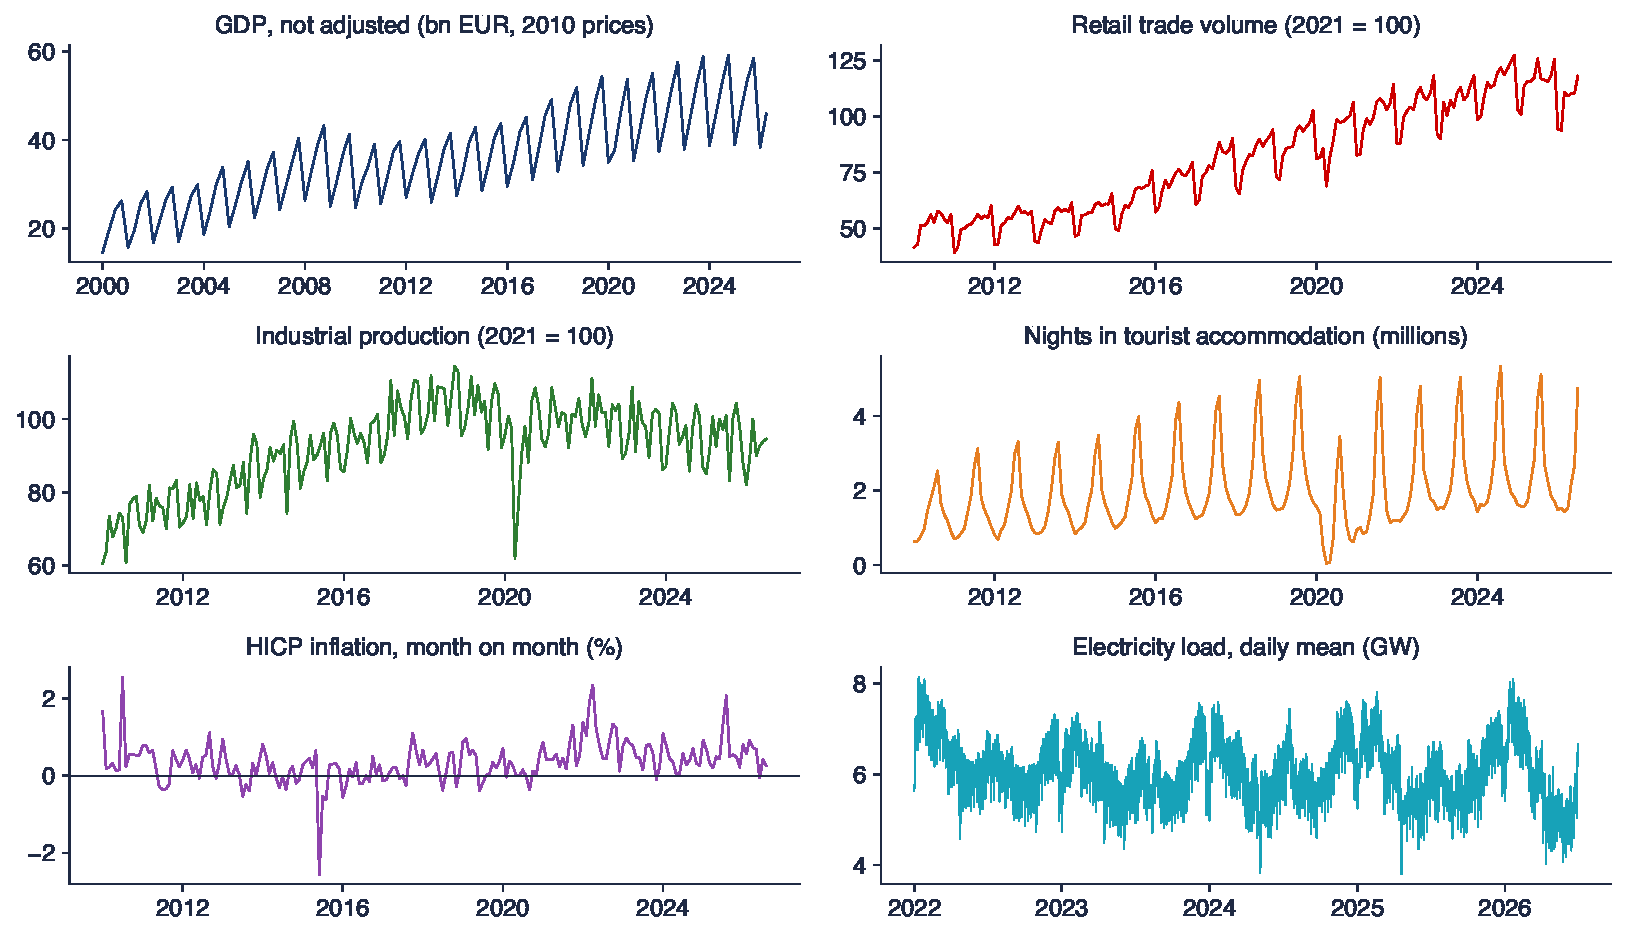
\includegraphics[width=0.97\textwidth,height=0.70\textheight,keepaspectratio]{tsa_ch4_series.pdf}
\end{center}
\vspace{-0.25cm}
\begin{itemize}
    \item Eurostat: GDP (quarterly, not adjusted), retail trade, industrial production, tourism nights, HICP; ENTSO-E: daily electricity load
\end{itemize}
\quantlet{TSA\_ch4\_seasonal\_data}{\qlurl{TSA_ch4_seasonal_data}}
\end{frame}

\begin{frame}{Interpreting the six series}
\itemsize{\footnotesize}
\begin{itemize}
    \item GDP: the mean of Q4 is 57\% above the mean of Q1 (2000--2026); the swing grows with the level: multiplicative, take logs
    \begin{itemize}
        \item quarter means (bn EUR, 2010 prices): 27.8, 33.6, 39.5, 43.6: construction and agriculture in Q2--Q3
    \end{itemize}
    \item Tourism: August has 3.7 times the nights of January (2015--2019); the 2020 lockdown breaks the pattern
    \item HICP: monthly inflation is lower in June (\ensuremath{-}0.37\% on average, 2010--2019, fresh food) and higher in October (0.49\%)
    \item Electricity: two patterns at once, the week (dense oscillation) and the year (winter peaks): \textbf{multiple seasonality}, Section 8
\end{itemize}
\end{frame}

\begin{frame}{Seasonal plot and subseries plot}
\itemsize{\footnotesize}
\begin{center}
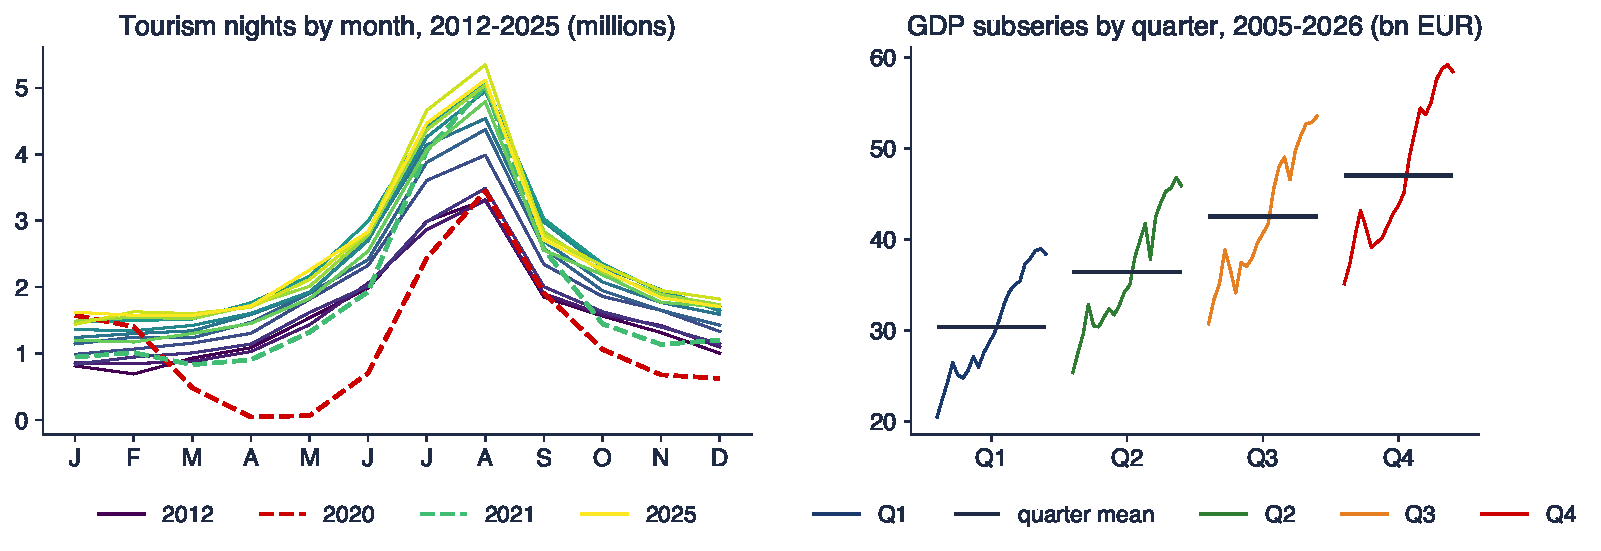
\includegraphics[width=0.97\textwidth,height=0.62\textheight,keepaspectratio]{tsa_ch4_seasonal_plot.pdf}
\end{center}
\vspace{-0.25cm}
\begin{itemize}
    \item Left: one line per year (seasonal plot); right: each quarter of GDP followed over the years, with its mean (subseries plot)
\end{itemize}
\quantlet{TSA\_ch4\_seasonal\_data}{\qlurl{TSA_ch4_seasonal_data}}
\end{frame}

\begin{frame}{Interpreting the seasonal plots}
\itemsize{\footnotesize}
\begin{columns}[T]
\begin{column}{0.58\textwidth}
\begin{itemize}
    \item Tourism: one shape every year, a summer peak and a winter trough
    \begin{itemize}
        \item 2019: 5.06 million nights in August, 1.47 million in January
        \item April 2020: 0.045 million (1.76 million in April 2019): an outlier, not a new season
    \end{itemize}
    \item GDP subseries: all four quarters rise in parallel
    \begin{itemize}
        \item a stable seasonal shape on top of a common trend
        \item if the lines crossed, the seasonal pattern would be changing: stochastic seasonality (next section)
    \end{itemize}
\end{itemize}
\end{column}
\begin{column}{0.38\textwidth}
\centering
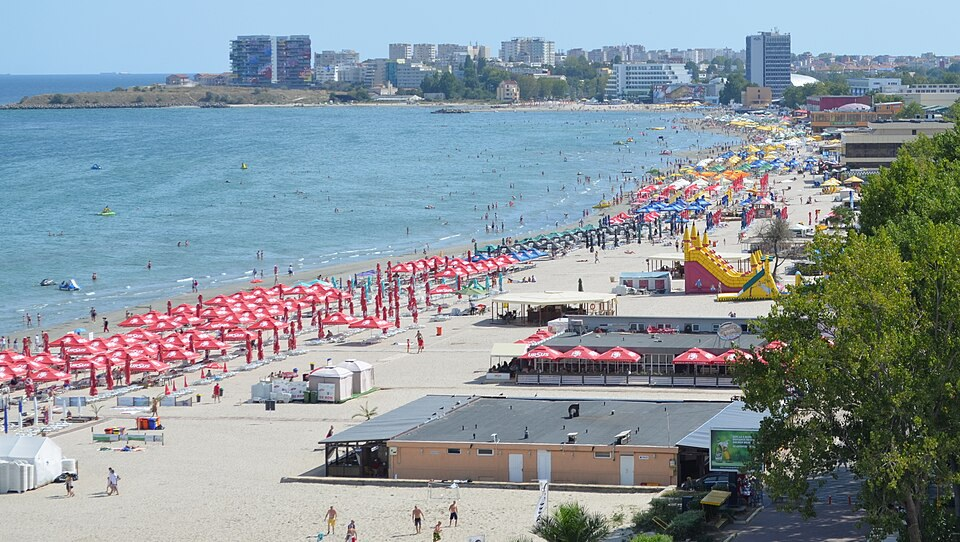
\includegraphics[height=0.36\textheight]{ch4_mamaia_2013.jpg}\\[1mm]
\imgcap{Mamaia, on the Black Sea, September 2013}
\imgcredit{https://commons.wikimedia.org/wiki/File:Mamaia_Beach_(September_2013).JPG}{Photo: Razvan Socol (2013); CC BY-SA 4.0; Wikimedia Commons}
\end{column}
\end{columns}
\end{frame}

\begin{frame}{Recap: Seasonality in economic data}
\itemsize{\small}
\begin{itemize}
    \item Seasonality repeats with a known period $s$; a cycle does not
    \item Weather, the calendar and institutions create it; moving holidays shift it between months
    \item Romanian GDP, tourism, inflation and electricity load are all seasonal; electricity has several periods at once
    \item Seasonal and subseries plots show whether the pattern is stable
\end{itemize}
\end{frame}


%=============================================================================
\section{Seasonal differencing and seasonal unit roots}
%=============================================================================

\begin{frame}{The seasonal difference}
\itemsize{\small}
\begin{itemize}
    \item \textbf{Seasonal difference}: $\Delta_s y_t = (1 - L^s)y_t = y_t - y_{t-s}$
    \begin{itemize}
        \item with logs: $100\,\Delta_4\ln Y_t$ = growth over the same quarter of the previous year, in \%
    \end{itemize}
    \item A \textbf{fixed} seasonal pattern $S_t = S_{t-s}$ plus a linear trend: $y_t = a + bt + S_t + \varepsilon_t$
    \begin{itemize}
        \item $a$: the intercept; $b$: the slope of the trend; $S_t$: the seasonal effect of period $t$
        \item $\Delta_s y_t = bs + \varepsilon_t - \varepsilon_{t-s}$: $\Delta_s$ removes the pattern and turns the trend into a constant
        \item but it creates the non-invertible MA term $\varepsilon_t - \varepsilon_{t-s}$: \textbf{seasonal over-differencing} (as in \tsachlink{https://danpele.github.io/Time-Series-Analysis/EN/Courses/chapter3_unit_roots_arima_models.pdf}{Chapter 3})
    \end{itemize}
    \item $\Delta\Delta_s = (1 - L)(1 - L^s) = 1 - L - L^s + L^{s+1}$: needed when the trend is stochastic as well
    \begin{itemize}
        \item the order of the two differences does not matter: the operators commute
    \end{itemize}
\end{itemize}
\end{frame}

\begin{frame}{Deterministic and stochastic seasonality}
\itemsize{\small}
\begin{itemize}
    \item \textbf{Deterministic}: $y_t = \sum_{j=1}^{s}\gamma_jD_{jt} + u_t$, with $D_{jt} = 1$ in season $j$ and $u_t$ stationary
    \begin{itemize}
        \item the seasonal means $\gamma_j$ never change; the right tool: seasonal dummies or Fourier terms (Section 7)
    \end{itemize}
    \item \textbf{Stochastic}: the \textbf{seasonal random walk} $y_t = y_{t-s} + \varepsilon_t$
    \begin{itemize}
        \item each season is its own random walk: $s$ separate walks interleaved
        \item $\mathrm{Var}(y_t)$ grows without bound; the pattern drifts, and ``summer can become winter''
        \item the right tool: the seasonal difference $\Delta_s$
    \end{itemize}
    \item The choice matters: differencing a deterministic pattern over-differences; modelling a stochastic one with dummies leaves a unit root in the residuals
\end{itemize}
\end{frame}

\begin{frame}{The roots of $1 - z^s$: seasonal unit roots}
\itemsize{\footnotesize}
\begin{center}
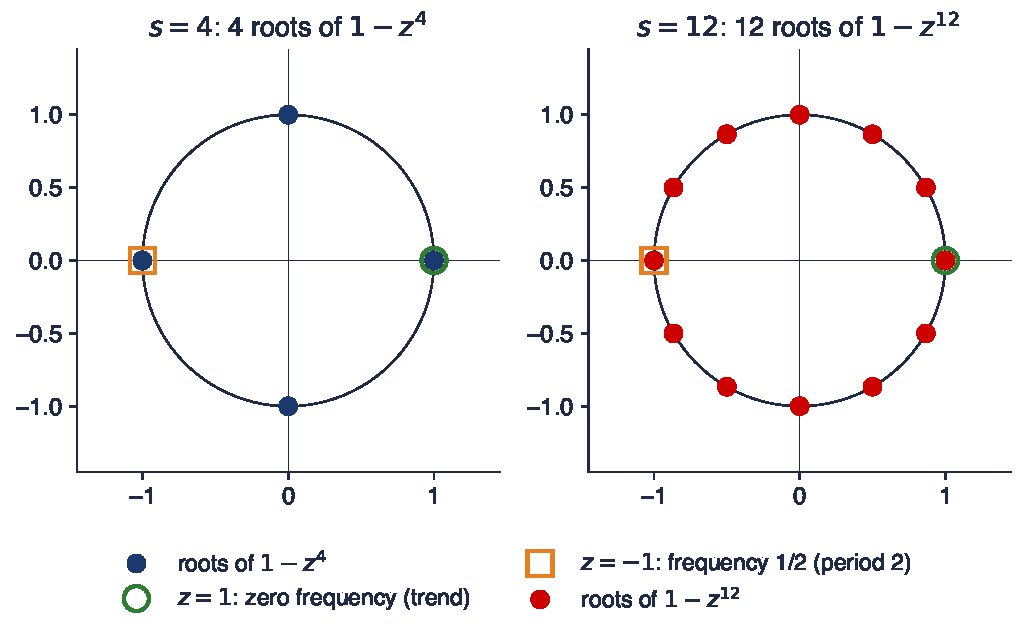
\includegraphics[width=0.97\textwidth,height=0.58\textheight,keepaspectratio]{tsa_ch4_unit_circle.pdf}
\end{center}
\vspace{-0.25cm}
\begin{itemize}
    \item $1 - z^4 = (1 - z)(1 + z)(1 + z^2)$: roots $1$, $-1$, $\pm i$, all on the unit circle
\end{itemize}
\quantlet{TSA\_ch4\_seasonal\_roots}{\qlurl{TSA_ch4_seasonal_roots}}
\end{frame}

\begin{frame}{Interpreting the seasonal roots}
\itemsize{\small}
\begin{itemize}
    \item $\Delta_s$ imposes $s$ unit roots at once, one for each \textbf{frequency} $k/s$, $k = 0, \dots, s - 1$
    \begin{itemize}
        \item quarterly: $z = 1$ (frequency 0, the trend), $z = -1$ (half a cycle per quarter: period 2 quarters), $z = \pm i$ (period 4 quarters: the annual cycle)
    \end{itemize}
    \item A series may have some of these roots and not others: then $\Delta_4$ over-differences at the frequencies it does not need
    \item Seasonal unit-root tests ask, frequency by frequency, which roots are present: the HEGY test (next slides)
\end{itemize}
\end{frame}

\begin{frame}{Romanian GDP: regular and seasonal differences}
\itemsize{\footnotesize}
\begin{center}
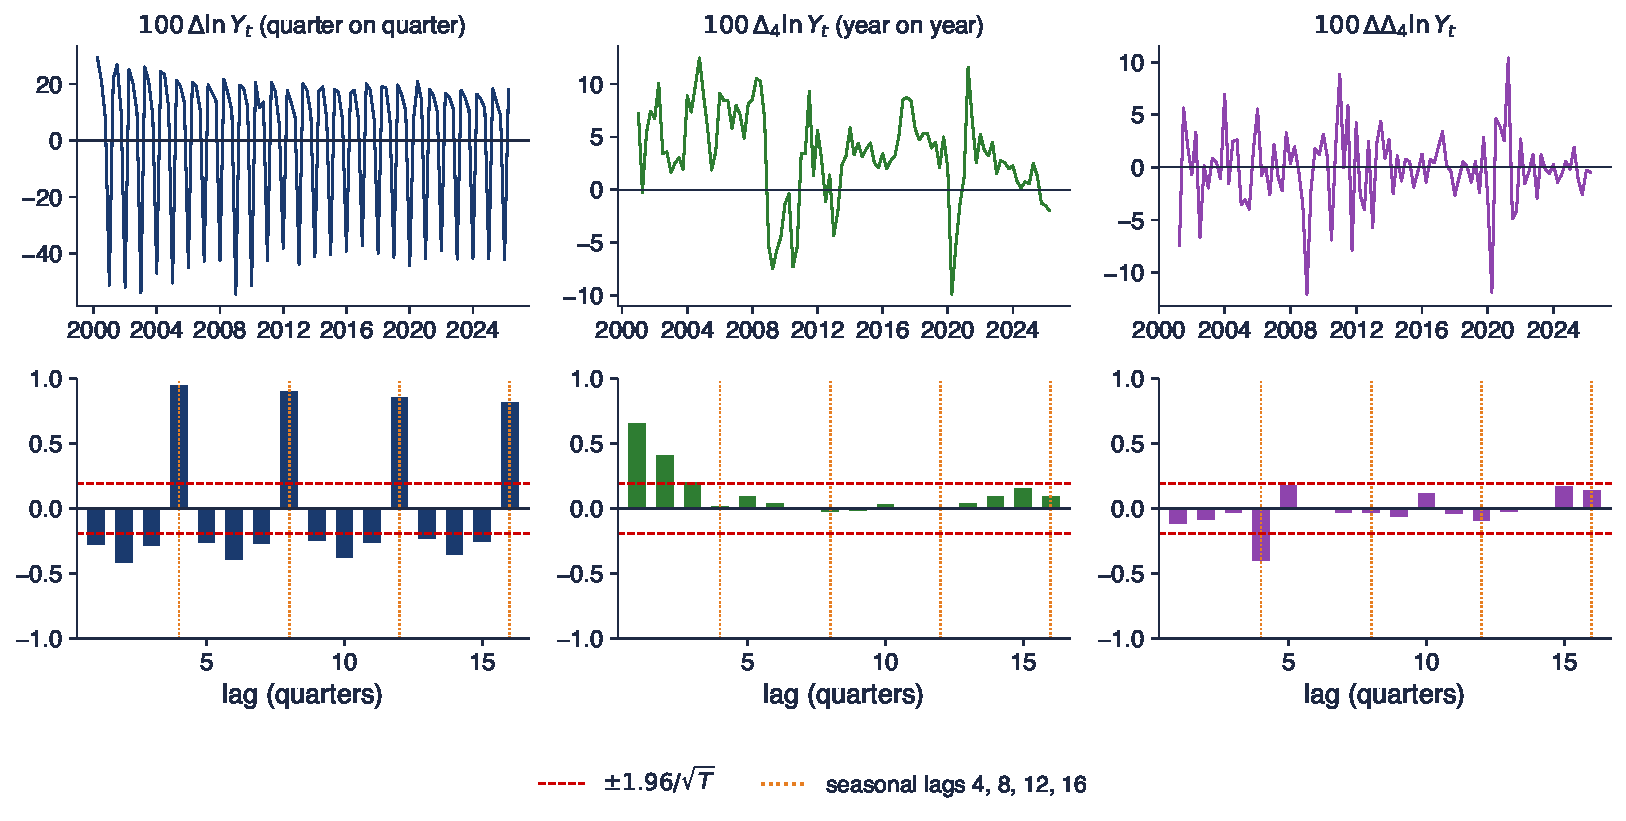
\includegraphics[width=0.97\textwidth,height=0.66\textheight,keepaspectratio]{tsa_ch4_gdp_diff.pdf}
\end{center}
\vspace{-0.25cm}
\begin{itemize}
    \item $\ln$ of real GDP, not adjusted, 106 quarters to 2026Q2; top: three transformations; bottom: their sample ACF up to 16 quarters
\end{itemize}
\quantlet{TSA\_ch4\_seasonal\_roots}{\qlurl{TSA_ch4_seasonal_roots}}
\end{frame}

\begin{frame}{Interpreting the three transformations}
\itemsize{\footnotesize}
\begin{itemize}
    \item $\Delta\ln Y$: dominated by the season: ACF $0.95$ at lag 4 and $0.90$ at lag 8, decaying very slowly; sd 26.5\%
    \begin{itemize}
        \item the seasonal analogue of the slow ACF decay of a random walk (\tsachlink{https://danpele.github.io/Time-Series-Analysis/EN/Courses/chapter3_unit_roots_arima_models.pdf}{Chapter 3})
    \end{itemize}
    \item $\Delta_4\ln Y$ (year-on-year growth): sd 4.4\%; ACF $0.66$ at lag 1, $0.01$ at lag 4: an AR-type pattern
    \item $\Delta\Delta_4\ln Y$: ACF $\ensuremath{-}0.11$ at lag 1 and $\ensuremath{-}0.40$ at lag 4 (band $\pm 0.20$)
    \begin{itemize}
        \item one negative spike at the seasonal lag: a seasonal MA(1), the signature of the airline model (Section 3)
    \end{itemize}
\end{itemize}
\end{frame}

\begin{frame}{The HEGY test}
\itemsize{\footnotesize}
\begin{columns}[T]
\begin{column}{0.64\textwidth}
\begin{itemize}
    \item \refHEGY: one regression tests every seasonal root of a quarterly series
    \begin{itemize}
        \item filters: $y_{1t} = (1 + L + L^2 + L^3)y_t$, $y_{2t} = -(1 - L + L^2 - L^3)y_t$, $y_{3t} = -(1 - L^2)y_t$
    \end{itemize}
    \item $\Delta_4y_t = \pi_1y_{1,t-1} + \pi_2y_{2,t-1} + \pi_3y_{3,t-2} + \pi_4y_{3,t-1} + \text{deterministic terms} + \text{lags of } \Delta_4y_t + \varepsilon_t$
    \begin{itemize}
        \item $y_{1t}, y_{2t}, y_{3t}$: the series filtered so that each keeps one seasonal frequency; $\pi_k$: the coefficient of each frequency
        \item $H_0$: $\pi_1 = 0$ (root $1$), $t$-test; $\pi_2 = 0$ (root $-1$), $t$-test; $\pi_3 = \pi_4 = 0$ (roots $\pm i$), $F$-test
        \item non-standard distributions, as for Dickey--Fuller: critical values from tables or by simulation
    \end{itemize}
    \item Rejecting all three: no seasonal differencing needed; rejecting none: $\Delta_4$ is justified
\end{itemize}
\end{column}
\begin{column}{0.32\textwidth}
\centering
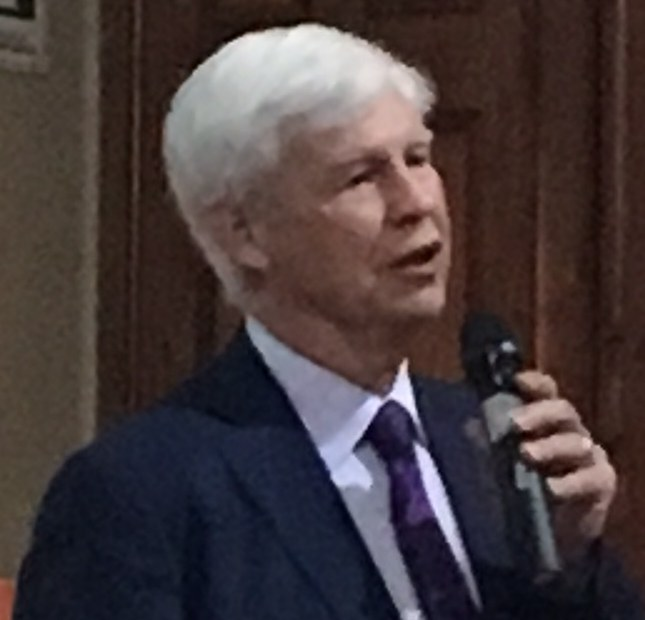
\includegraphics[height=0.40\textheight]{ch4_robert_engle_2017.jpg}\\[1mm]
\imgcap{Robert Engle, a co-author of HEGY, 2017}
\imgcredit{https://commons.wikimedia.org/wiki/File:Robert_Engle_SantiagoWEAI2017.png}{Photo: Econterms (2017); CC BY-SA 4.0; Wikimedia Commons}
\end{column}
\end{columns}
\end{frame}

\begin{frame}{Canova--Hansen and OCSB}
\itemsize{\small}
\begin{itemize}
    \item \textbf{Canova--Hansen} (\refCH): the null is \textbf{stable} (deterministic) seasonality
    \begin{itemize}
        \item the seasonal analogue of KPSS (\tsachlink{https://danpele.github.io/Time-Series-Analysis/EN/Courses/chapter3_unit_roots_arima_models.pdf}{Chapter 3}): rejecting means the pattern changes over time
    \end{itemize}
    \item \textbf{OCSB} (\refOCSB): the null is a seasonal unit root; a regression of $\Delta\Delta_s y_t$ on $\Delta_s y_{t-1}$ and $\Delta y_{t-s}$
    \begin{itemize}
        \item the default seasonal test of \texttt{auto\_arima} in the Python package \texttt{pmdarima} (\texttt{nsdiffs})
    \end{itemize}
    \item As in \tsachlink{https://danpele.github.io/Time-Series-Analysis/EN/Courses/chapter3_unit_roots_arima_models.pdf}{Chapter 3}: tests with opposite nulls answer different questions; use them together
    \begin{itemize}
        \item and look at the data: seasonal plots, the ACF at lags $s, 2s, 3s$, and the size of $\hat\Theta$ after $\Delta_s$ ($\hat\Theta \approx -1$ signals over-differencing)
    \end{itemize}
\end{itemize}
\end{frame}

\begin{frame}{Seasonal unit-root tests on Romanian data}
\itemsize{\scriptsize}
\begin{center}
\scriptsize
\begin{tabular}{lrrr}
\toprule
\textbf{HEGY}, $\ln$ GDP, 2000--2019 & statistic & 5\% critical value & decision \\
\midrule
$t(\pi_1)$, root $1$ & $\ensuremath{-}1.97$ & $\ensuremath{-}3.39$ & not rejected \\
$t(\pi_2)$, root $-1$ & $\ensuremath{-}2.19$ & $\ensuremath{-}2.77$ & not rejected \\
$F(\pi_3, \pi_4)$, roots $\pm i$ & $6.12$ & $6.64$ & not rejected \\
\bottomrule
\end{tabular}
\end{center}
\begin{center}
\scriptsize
\begin{tabular}{lccc}
\toprule
\textbf{Series} (logs, 2005--2019) & $D$ by OCSB & $D$ by Canova--Hansen & $d$ by KPSS \\
\midrule
GDP (quarterly) & 1 & 0 & 1 \\
Retail trade & 0 & 0 & 1 \\
Industrial production & 0 & 0 & 1 \\
Tourism nights & 0 & 0 & 1 \\
HICP & 0 & 0 & 2 \\
\bottomrule
\end{tabular}
\end{center}
\begin{itemize}
    \item HEGY: constant, seasonal dummies and trend, 1 lag of $\Delta_4y$ (AIC), $n = 75$; critical values from 4\,000 simulations of $\Delta_4y_t = \varepsilon_t$
    \item Interpretation: for GDP, HEGY and OCSB support $\Delta_4$ while Canova--Hansen does not reject a stable pattern; with 20 years of quarters both views fit, so we use $\Delta_4$ and let $\hat\Theta$ say how stable the pattern is (Section 5)
    \item Monthly series: both tests choose $D = 0$, a stable pattern; HICP needs $d = 2$ in logs: inflation itself is close to a unit root (\tsachlink{https://danpele.github.io/Time-Series-Analysis/EN/Courses/chapter3_unit_roots_arima_models.pdf}{Chapter 3})
\end{itemize}
\end{frame}

\begin{frame}{Recap: Seasonal differencing and seasonal unit roots}
\itemsize{\small}
\begin{itemize}
    \item $\Delta_s = 1 - L^s$ has $s$ unit roots on the circle, one per seasonal frequency
    \item Deterministic seasonality: dummies or Fourier terms; stochastic seasonality: $\Delta_s$
    \item HEGY and OCSB test for seasonal unit roots; Canova--Hansen tests for a stable pattern
    \item Romanian GDP: $\Delta\Delta_4\ln Y$ leaves one spike at lag 4, a seasonal MA
\end{itemize}
\end{frame}


%=============================================================================
\section{SARIMA models}
%=============================================================================

\begin{frame}{The SARIMA$(p,d,q)(P,D,Q)_s$ model}
\itemsize{\small}
\begin{itemize}
    \item $\phi(L)\,\Phi(L^s)\,(1 - L)^d(1 - L^s)^D\,y_t = c + \theta(L)\,\Theta(L^s)\,\varepsilon_t$, $\varepsilon_t \sim \mathrm{WN}(0, \sigma^2)$
    \begin{itemize}
        \item regular polynomials $\phi(L)$ (order $p$), $\theta(L)$ (order $q$), as in \tsachlink{https://danpele.github.io/Time-Series-Analysis/EN/Courses/chapter2_arma_models.pdf}{Chapter 2}
        \item seasonal polynomials in $L^s$ (orders $P$, $Q$): $\Phi(L^s) = 1 - \Phi_1L^s - \dots - \Phi_PL^{Ps}$, $\Theta(L^s) = 1 + \Theta_1L^s + \dots + \Theta_QL^{Qs}$
        \item $d$, $D$: numbers of regular and seasonal differences, usually 0 or 1
    \end{itemize}
    \item Why multiply? \refBJ: in a monthly series, January depends on December (the regular part) and on last January (the seasonal part)
    \begin{itemize}
        \item a two-way table: months in the columns, years in the rows; one model along each direction
    \end{itemize}
    \item Stationarity: the roots of $\phi(z)\Phi(z^s)$ outside the unit circle; invertibility: the roots of $\theta(z)\Theta(z^s)$ outside; for a seasonal AR(1) this means $|\Phi| < 1$
\end{itemize}
\end{frame}

\begin{frame}{Worked example: the airline model}
\itemsize{\small}
\begin{itemize}
    \item SARIMA$(0,1,1)(0,1,1)_{12}$ with $\theta = -0.4$, $\Theta = -0.6$: $(1 - L)(1 - L^{12})y_t = (1 - 0.4L)(1 - 0.6L^{12})\varepsilon_t$
    \begin{itemize}
        \item left: $y_t - y_{t-1} - y_{t-12} + y_{t-13}$; right: $\varepsilon_t - 0.4\varepsilon_{t-1} - 0.6\varepsilon_{t-12} + 0.24\varepsilon_{t-13}$
        \item the coefficient of $\varepsilon_{t-13}$, $\theta\Theta = 0.24$, is not a new parameter: two parameters plus $\sigma^2$
    \end{itemize}
    \item $w_t = \Delta\Delta_{12}y_t$ is an MA(13) with only four nonzero weights; its autocovariances (\tsachlink{https://danpele.github.io/Time-Series-Analysis/EN/Courses/chapter2_arma_models.pdf}{Chapter 2}):
    \begin{itemize}
        \item $\gamma(0) = \sigma^2(1 + \theta^2)(1 + \Theta^2) = 1.5776\,\sigma^2$
        \item $\rho_1 = \theta/(1 + \theta^2) = \ensuremath{-}0.345$; $\rho_{12} = \Theta/(1 + \Theta^2) = \ensuremath{-}0.441$; $\rho_{11} = \rho_{13} = \rho_1\rho_{12} = 0.152$
        \item all other autocorrelations are zero
    \end{itemize}
\end{itemize}
\end{frame}

\begin{frame}{Theoretical ACF and PACF of three seasonal models}
\itemsize{\footnotesize}
\begin{center}
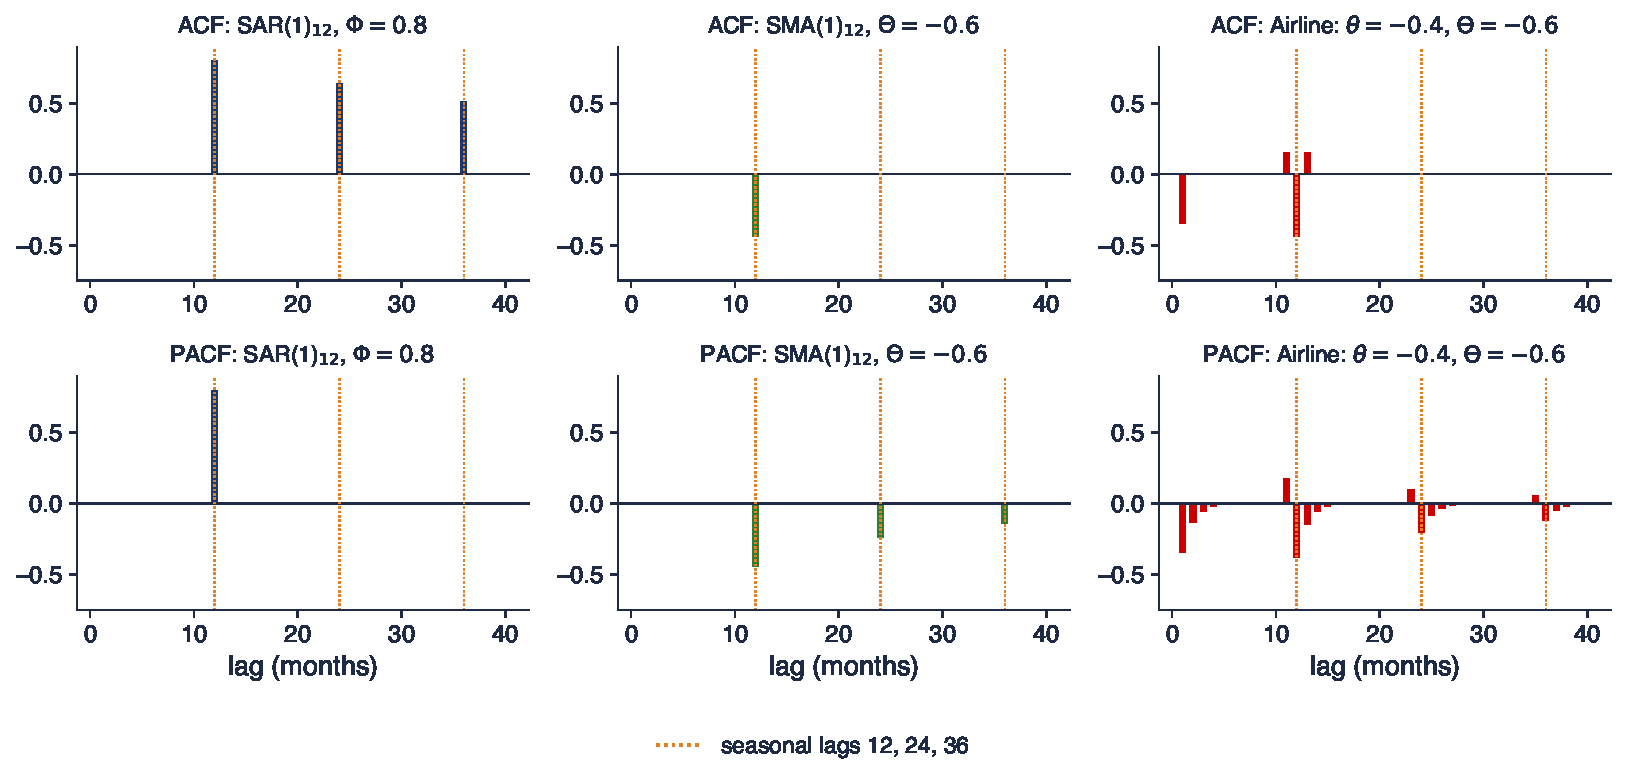
\includegraphics[width=0.97\textwidth,height=0.66\textheight,keepaspectratio]{tsa_ch4_theory_acf.pdf}
\end{center}
\vspace{-0.25cm}
\begin{itemize}
    \item Monthly, $s = 12$; the airline panel is the stationary part $w_t = \Delta\Delta_{12}y_t$
\end{itemize}
\quantlet{TSA\_ch4\_sarima\_theory}{\qlurl{TSA_ch4_sarima_theory}}
\end{frame}

\begin{frame}{Interpreting the seasonal patterns}
\itemsize{\small}
\begin{itemize}
    \item Seasonal AR(1): the ACF decays geometrically at lags 12, 24, 36 ($0.8$, $0.64$, $0.512$); the PACF has one spike at lag 12
    \begin{itemize}
        \item the AR rule of \tsachlink{https://danpele.github.io/Time-Series-Analysis/EN/Courses/chapter2_arma_models.pdf}{Chapter 2}, read only at multiples of $s$
    \end{itemize}
    \item Seasonal MA(1): the ACF cuts off after lag 12; the PACF decays at 12, 24, 36 (\ensuremath{-}0.242 at lag 24)
    \item Airline: spikes at 1 (\ensuremath{-}0.345) and 12 (\ensuremath{-}0.441), with ``satellites'' at 11 and 13 (0.152)
    \begin{itemize}
        \item the satellites are the product $\rho_1\rho_{12}$: the fingerprint of the multiplicative structure
    \end{itemize}
\end{itemize}
\end{frame}

\begin{frame}{Identification of SARIMA models}
\itemsize{\footnotesize}
\begin{center}
\footnotesize
\begin{tabular}{lll}
\toprule
\textbf{After differencing} & \textbf{ACF} & \textbf{PACF} \\
\midrule
seasonal AR($P$) & decays at $s, 2s, \dots$ & cuts off after lag $Ps$ \\
seasonal MA($Q$) & cuts off after lag $Qs$ & decays at $s, 2s, \dots$ \\
regular part & lags $1, 2, \dots$ as in \tsachlink{https://danpele.github.io/Time-Series-Analysis/EN/Courses/chapter2_arma_models.pdf}{Chapter 2} & lags $1, 2, \dots$ as in \tsachlink{https://danpele.github.io/Time-Series-Analysis/EN/Courses/chapter2_arma_models.pdf}{Chapter 2} \\
product of both & satellites at $ks \pm j$ & satellites at $ks \pm j$ \\
\bottomrule
\end{tabular}
\end{center}
\begin{itemize}
    \item \textbf{Steps}
    \begin{itemize}
        \item 1. Stabilise the variance (logs or Box--Cox, \refBoxCox); 2. choose $D$ (seasonal plot, HEGY, OCSB), then $d$ (\tsachlink{https://danpele.github.io/Time-Series-Analysis/EN/Courses/chapter3_unit_roots_arima_models.pdf}{Chapter 3})
        \item 3. Read $P, Q$ at the seasonal lags and $p, q$ at the first lags; 4. keep the orders small: $P, Q \le 1$ almost always suffice
    \end{itemize}
\end{itemize}
\end{frame}

\begin{frame}{Estimation and model choice}
\itemsize{\small}
\begin{itemize}
    \item \textbf{Maximum likelihood} of the differenced series (state-space form, \texttt{statsmodels} \texttt{SARIMAX})
    \begin{itemize}
        \item $s + 1$ observations are lost to $\Delta\Delta_s$; the constant is dropped when $d + D \ge 2$ (it would mean a quadratic trend)
    \end{itemize}
    \item \textbf{Information criteria}: AICc $=$ AIC $+ \frac{2k(k + 1)}{n - k - 1}$ and BIC, compared \textbf{only} across models with the same $d$ and $D$
    \begin{itemize}
        \item $k$: the number of estimated parameters; $n$: the number of observations after differencing
        \item differencing changes the data on which the likelihood is computed
    \end{itemize}
    \item \textbf{Automatic SARIMA}: a stepwise search over $(p, q, P, Q)$ by AICc after choosing $d$ and $D$ by tests (\refHK)
    \begin{itemize}
        \item in Python: \texttt{pmdarima.auto\_arima(y, m=12)}; always check the residuals and compare with a benchmark
    \end{itemize}
    \item \textbf{Diagnostics}: Ljung--Box with lags beyond $s$ (e.g. $m = 2s$) and $m - p - q - P - Q$ degrees of freedom (\refLB)
\end{itemize}
\end{frame}

\begin{frame}{Forecasting with SARIMA}
\itemsize{\small}
\begin{itemize}
    \item As for ARIMA (\tsachlink{https://danpele.github.io/Time-Series-Analysis/EN/Courses/chapter3_unit_roots_arima_models.pdf}{Chapter 3}): write the model as an equation for $y_t$; replace future shocks by 0, future values by their forecasts, past shocks by residuals
    \begin{itemize}
        \item airline: $\hat y_{T+h} = \hat y_{T+h-1} + \hat y_{T+h-s} - \hat y_{T+h-s-1} + (\text{MA terms while } h \le s + 1)$
    \end{itemize}
    \item \textbf{Eventual forecast function} of the airline model: a fixed seasonal pattern on a straight line
    \begin{itemize}
        \item the pattern is an exponentially weighted average of past patterns, with weight $1 + \Theta$ on the most recent year
        \item $\Theta \to -1$: a fixed (deterministic) pattern; $\Theta = 0$: last year's pattern repeated (seasonal naive)
    \end{itemize}
    \item Intervals widen with $h$ (two unit roots); for $\ln y$, $\exp(\hat y_{T+h})$ is the forecast \textbf{median}
    \begin{itemize}
        \item the mean is $\exp(\hat y_{T+h} + \sigma_h^2/2)$, slightly higher; $\sigma_h^2$: the forecast error variance at horizon $h$
    \end{itemize}
\end{itemize}
\end{frame}

\begin{frame}{Worked example: forecasting a seasonal MA}
\itemsize{\small}
\begin{itemize}
    \item Quarterly SARIMA$(0,0,0)(0,1,1)_4$: $y_t = y_{t-4} + \varepsilon_t + \Theta\varepsilon_{t-4}$, $\Theta = -0.6$
    \begin{itemize}
        \item last year: $y_{T-3}, \dots, y_T = 100, 120, 130, 140$; residuals $\hat\varepsilon_{T-3}, \dots, \hat\varepsilon_T = 2, -1, 0, 3$
    \end{itemize}
    \item $\hat y_{T+1} = y_{T-3} + \Theta\hat\varepsilon_{T-3} = 100 - 0.6 \cdot 2 = 98.8$
    \begin{itemize}
        \item $\hat y_{T+2} = 120.6$, $\hat y_{T+3} = 130.0$, $\hat y_{T+4} = 138.2$
    \end{itemize}
    \item $\hat y_{T+5} = \hat y_{T+1} = 98.8$: after one year the MA term is gone and the forecast pattern repeats
    \begin{itemize}
        \item a large positive surprise last season ($\hat\varepsilon_T = 3$) lowers the forecast for that season by $0.6 \cdot 3$: partial correction
    \end{itemize}
\end{itemize}
\end{frame}

\begin{frame}{Recap: SARIMA models}
\itemsize{\small}
\begin{itemize}
    \item SARIMA multiplies regular and seasonal polynomials: $\phi(L)\Phi(L^s)\Delta^d\Delta_s^Dy_t = \theta(L)\Theta(L^s)\varepsilon_t$
    \item Identification: the \tsachlink{https://danpele.github.io/Time-Series-Analysis/EN/Courses/chapter2_arma_models.pdf}{Chapter 2} rules at lags $s, 2s, \dots$, plus satellites at $ks \pm j$
    \item Compare AICc only for the same $d$ and $D$; check Ljung--Box beyond lag $s$
    \item The airline forecast: a seasonal pattern on a line, updated with weight $1 + \Theta$
\end{itemize}
\end{frame}


%=============================================================================
\section{Case study: the airline model}
%=============================================================================

\begin{frame}{Box and Jenkins and the airline passengers}
\itemsize{\footnotesize}
\begin{columns}[T]
\begin{column}{0.56\textwidth}
\begin{itemize}
    \item \refBJ{} (first edition 1970) modelled the monthly totals of international airline passengers, 1949--1960 (144 months)
    \begin{itemize}
        \item growth plus a summer peak whose size grows with the level
        \item their model, SARIMA$(0,1,1)(0,1,1)_{12}$ for $\ln y_t$, has carried the name ``airline model'' ever since
    \end{itemize}
    \item Why it lasted
    \begin{itemize}
        \item two parameters fit many seasonal series: trade, production, retail sales, energy
        \item it is the reference model of the regARIMA step of seasonal-adjustment software (Section 6)
    \end{itemize}
\end{itemize}
\end{column}
\begin{column}{0.40\textwidth}
\centering
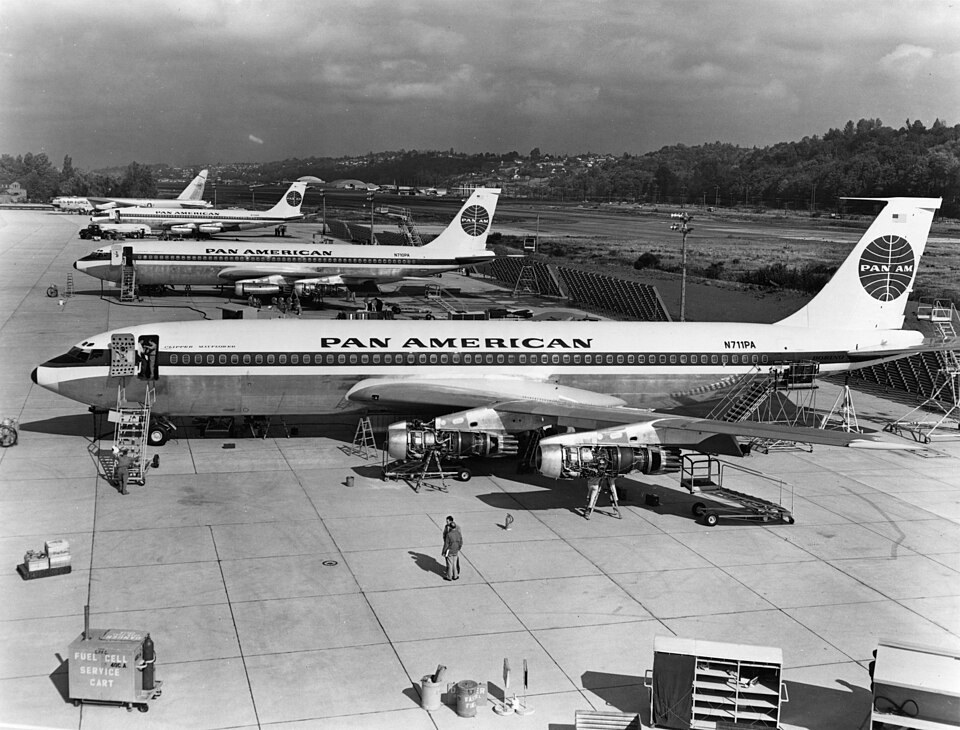
\includegraphics[height=0.36\textheight]{ch4_pan_am_707_1958.jpg}\\[1mm]
\imgcap{The first Boeing 707s for Pan American, Seattle, 1958}
\imgcredit{https://commons.wikimedia.org/wiki/File:Three_Pan_Am_Boeing_707_awaiting_delivery.jpg}{Photo: unknown author (1958); public domain; Wikimedia Commons}
\end{column}
\end{columns}
\end{frame}

\begin{frame}{Identification of the airline model}
\itemsize{\footnotesize}
\begin{center}
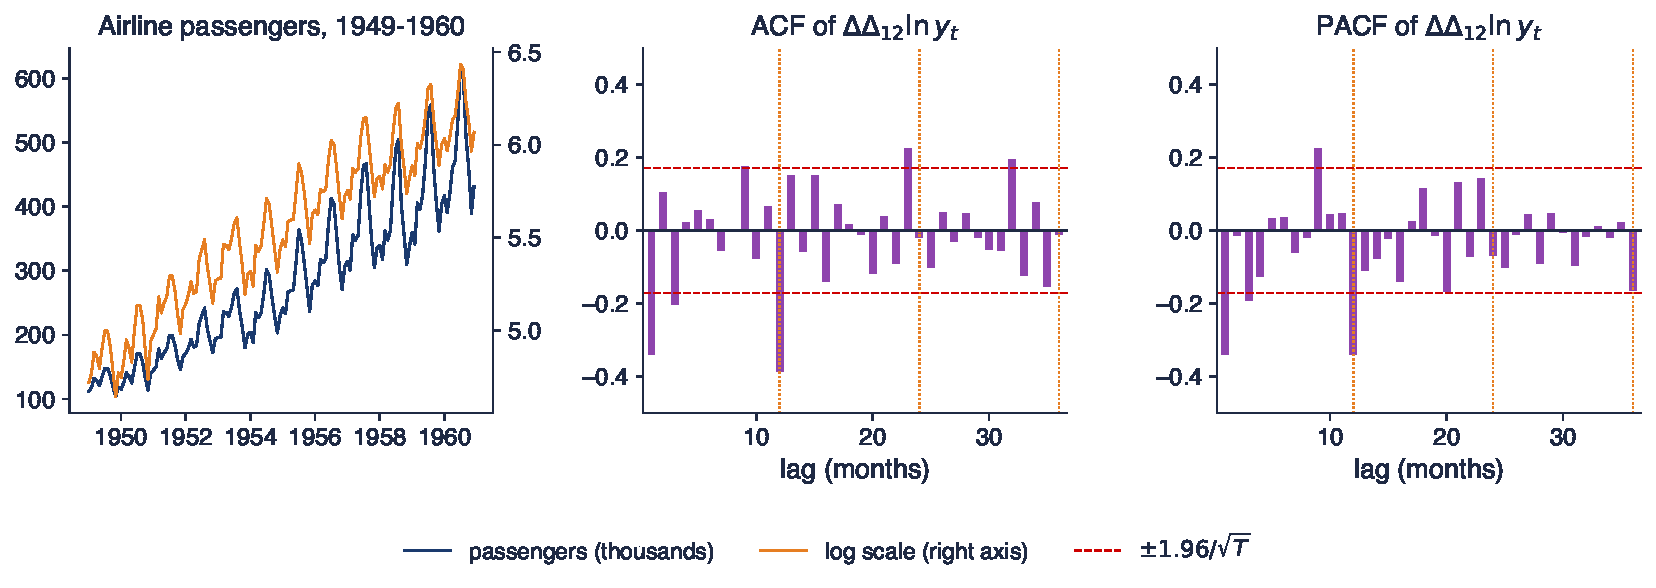
\includegraphics[width=0.97\textwidth,height=0.58\textheight,keepaspectratio]{tsa_ch4_airline.pdf}
\end{center}
\vspace{-0.25cm}
\begin{itemize}
    \item Left: passengers and their log; middle and right: ACF and PACF of $w_t = \Delta\Delta_{12}\ln y_t$, 131 observations
\end{itemize}
\quantlet{TSA\_ch4\_airline}{\qlurl{TSA_ch4_airline}}
\end{frame}

\begin{frame}{Interpreting the airline correlograms}
\itemsize{\small}
\begin{itemize}
    \item The log makes the summer swing constant: the multiplicative pattern becomes additive
    \item ACF of $w_t$: $\ensuremath{-}0.34$ at lag 1 and $\ensuremath{-}0.39$ at lag 12, outside the band $\pm 0.17$
    \begin{itemize}
        \item a regular MA(1) and a seasonal MA(1); lag 3 ($\ensuremath{-}0.20$) is borderline
    \end{itemize}
    \item The PACF decays at lags 1, 2, 3 and 12, 24: consistent with MA terms, not AR terms
    \item Conclusion: SARIMA$(0,1,1)(0,1,1)_{12}$, exactly the model of Box and Jenkins
\end{itemize}
\end{frame}

\begin{frame}{Airline model: forecasts out of sample}
\itemsize{\footnotesize}
\begin{center}
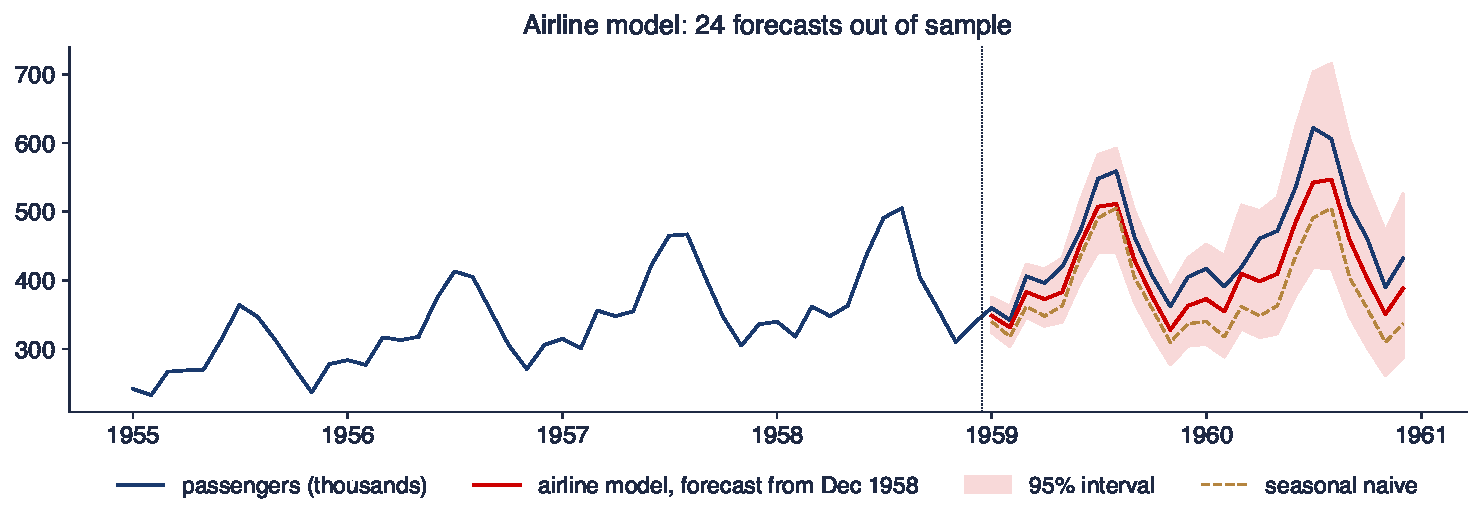
\includegraphics[width=0.97\textwidth,height=0.56\textheight,keepaspectratio]{tsa_ch4_airline_fc.pdf}
\end{center}
\vspace{-0.25cm}
\begin{itemize}
    \item Estimated on 1949--1958, forecasts for the 24 months of 1959--1960, back-transformed from $\ln y$
\end{itemize}
\quantlet{TSA\_ch4\_airline}{\qlurl{TSA_ch4_airline}}
\end{frame}

\begin{frame}{Interpreting the airline forecasts}
\itemsize{\footnotesize}
\begin{itemize}
    \item 1949--1958: $\hat\theta = \ensuremath{-}0.342$ (0.087), $\hat\Theta = \ensuremath{-}0.541$ (0.105); full sample: $\hat\theta = \ensuremath{-}0.402$ (0.073), $\hat\Theta = \ensuremath{-}0.557$ (0.096)
    \begin{itemize}
        \item residual sd 3.7\% per month; Ljung--Box $Q^*(24)$ on 22 degrees of freedom, p = 0.37
    \end{itemize}
    \item MAPE over 1959--1960: 8.5\% for the airline model, 15.5\% for the seasonal naive forecast (which ignores growth)
    \item December 1960: forecast 388, interval [286, 526], actual 432: inside, but the model under-predicts the 1959--1960 growth
    \begin{itemize}
        \item the interval width grows from 51 (first month) to 239 (24th month): two unit roots
    \end{itemize}
\end{itemize}
\end{frame}


%=============================================================================
\section{Case study: Romanian GDP, not adjusted}
%=============================================================================

\begin{frame}{SARIMA models for Romanian GDP}
\itemsize{\footnotesize}
\begin{center}
\scriptsize
\begin{tabular}{lrrrr}
\toprule
\textbf{Model} & \textbf{AICc} & \textbf{BIC} & \textbf{LB(8), p} & $\hat\sigma$ (\%) \\
\midrule
$(0,1,1)(0,1,1)_4$ & 520.1 & 527.6 & 0.157 & 3.05 \\
$(0,1,0)(0,1,1)_4$ & 519.7 & \textbf{524.8} & 0.286 & 3.08 \\
$(1,1,0)(0,1,1)_4$ & 520.7 & 528.3 & 0.156 & 3.06 \\
$(1,1,1)(0,1,1)_4$ & \textbf{518.3} & 528.4 & 0.467 & 2.98 \\
$(0,1,2)(0,1,1)_4$ & 518.8 & 528.8 & 0.575 & 3.00 \\
$(0,1,1)(1,1,0)_4$ & 529.9 & 537.5 & 0.003 & 3.22 \\
$(0,1,1)(1,1,1)_4$ & 522.2 & 532.2 & 0.118 & 3.05 \\
$(0,1,1)(0,1,0)_4$ & 545.1 & 550.2 & 0.005 & 3.52 \\
\bottomrule
\end{tabular}
\end{center}
\begin{itemize}
    \item $y_t = 100\ln Y_t$, real GDP not adjusted, 2000Q1--2026Q2, $T = 106$; maximum likelihood; all with $d = D = 1$, so the criteria are comparable
    \item Ljung--Box on 8 lags with $8 - p - q - P - Q$ degrees of freedom
\end{itemize}
\end{frame}

\begin{frame}{Interpreting the model table}
\itemsize{\small}
\begin{itemize}
    \item BIC chooses $(0,1,0)(0,1,1)_4$: only the seasonal MA term; AICc chooses $(1,1,1)(0,1,1)_4$
    \begin{itemize}
        \item the AICc model has $\hat\phi = 0.78$ and $\hat\theta = \ensuremath{-}0.94$: almost a common factor (\tsachlink{https://danpele.github.io/Time-Series-Analysis/EN/Courses/chapter2_arma_models.pdf}{Chapter 2}), little gain
        \item the airline model: $\hat\theta = \ensuremath{-}0.171$ (0.109), not significant; $\hat\Theta = \ensuremath{-}0.585$
    \end{itemize}
    \item A seasonal AR instead of the seasonal MA, or no seasonal term at all: much worse criteria and correlated residuals
    \item We keep the BIC model: one parameter, $\hat\Theta = \ensuremath{-}0.577$ (0.075), $\hat\sigma = 3.08\%$
\end{itemize}
\end{frame}

\begin{frame}{Diagnostics of the GDP model}
\itemsize{\footnotesize}
\begin{center}
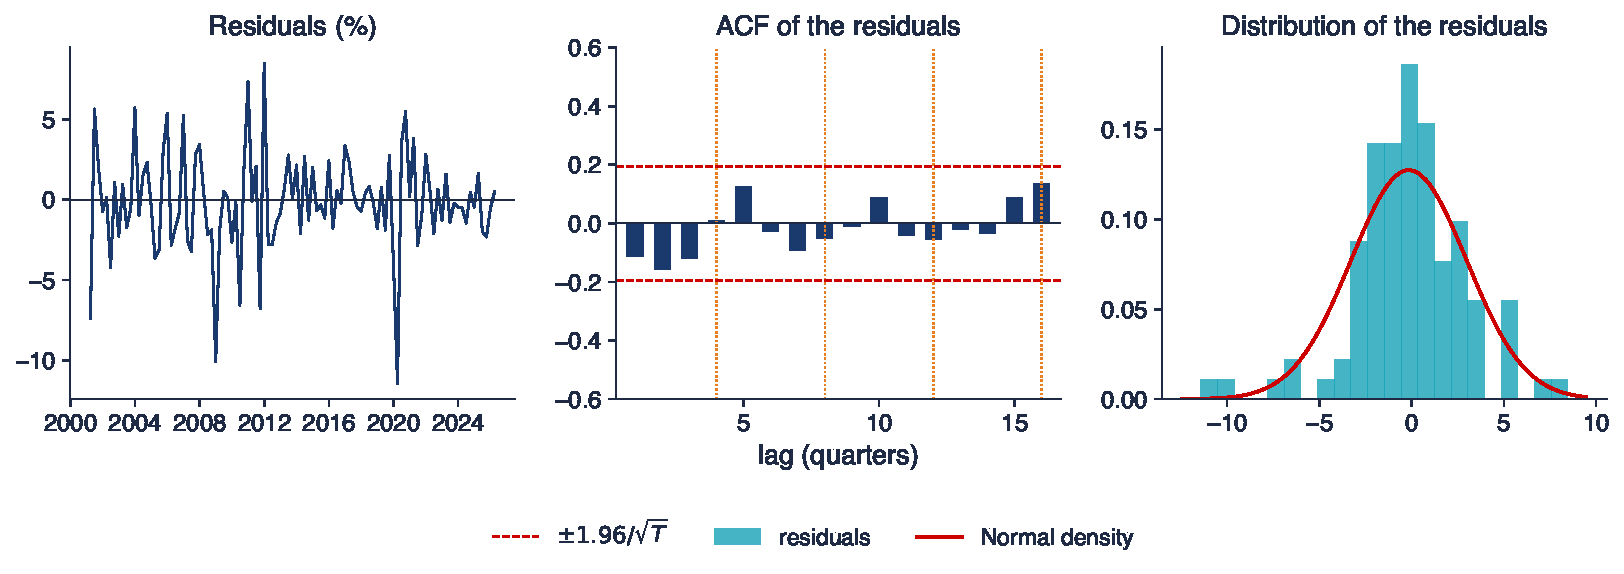
\includegraphics[width=0.97\textwidth,height=0.56\textheight,keepaspectratio]{tsa_ch4_gdp_diag.pdf}
\end{center}
\vspace{-0.25cm}
\begin{itemize}
    \item SARIMA$(0,1,0)(0,1,1)_4$ for $100\ln Y_t$: residuals, their ACF and their distribution
\end{itemize}
\quantlet{TSA\_ch4\_gdp\_case}{\qlurl{TSA_ch4_gdp_case}}
\end{frame}

\begin{frame}{Interpreting the GDP diagnostics}
\itemsize{\small}
\begin{itemize}
    \item No autocorrelation left: $Q^*(8) = 8.55$ on 7 degrees of freedom, p = 0.286; $Q^*(12)$: p = 0.526
    \begin{itemize}
        \item no spike at the seasonal lags 4, 8, 12, 16: the seasonal structure is captured
    \end{itemize}
    \item Not Normal: Jarque--Bera 22.0 (p $<$\,0.001); the largest residual is \ensuremath{-}11.4\% in 2020Q2 ($\ensuremath{-}3.6$ standard deviations): the lockdown
    \begin{itemize}
        \item without 2020, Jarque--Bera falls to 13.4: an additive-outlier dummy would be the next step
    \end{itemize}
\end{itemize}
\end{frame}

\begin{frame}{Forecasts of Romanian GDP}
\itemsize{\footnotesize}
\begin{center}
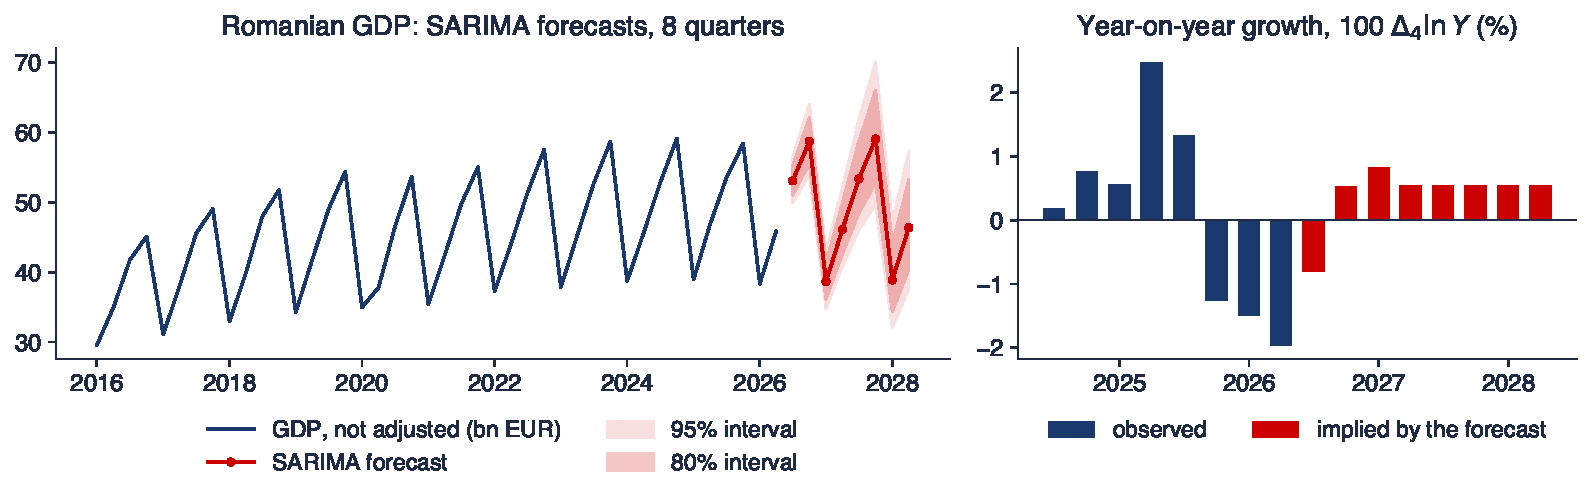
\includegraphics[width=0.97\textwidth,height=0.56\textheight,keepaspectratio]{tsa_ch4_gdp_fc.pdf}
\end{center}
\vspace{-0.25cm}
\begin{itemize}
    \item SARIMA$(0,1,0)(0,1,1)_4$, 8 quarters from 2026Q3 to 2028Q2, 80\% and 95\% intervals; right: implied year-on-year growth
\end{itemize}
\quantlet{TSA\_ch4\_gdp\_case}{\qlurl{TSA_ch4_gdp_case}}
\end{frame}

\begin{frame}{Interpreting the GDP forecasts}
\itemsize{\small}
\begin{itemize}
    \item Last value: 45.9 bn EUR in 2026Q2; forecasts 53.1, 58.7, 38.7, 46.1 bn EUR for the next four quarters
    \begin{itemize}
        \item 95\% interval for the first quarter [50.0, 56.4], for the eighth [37.6, 57.2]
    \end{itemize}
    \item Implied year-on-year growth: \ensuremath{-}0.81\%, 0.53\%, 0.83\%, 0.55\%, then a constant 0.55\%
    \begin{itemize}
        \item the model extrapolates the recent weak growth; it knows nothing about fiscal policy or EU funds
    \end{itemize}
    \item The seasonal pattern of the forecast is a weighted average of past years, with weight $1 + \hat\Theta = 0.42$ on the newest year
\end{itemize}
\end{frame}

\begin{frame}{Recap: Airline passengers and Romanian GDP}
\itemsize{\small}
\begin{itemize}
    \item Logs, then $\Delta\Delta_s$, then MA terms at lags 1 and $s$: the airline recipe works for both series
    \item For GDP, BIC drops the regular MA term; AICc picks a near-redundant ARMA(1,1)
    \item Residuals are clean except for the 2020 outlier
    \item Forecasts repeat a smoothed seasonal pattern on a trend line, with widening intervals
\end{itemize}
\end{frame}


%=============================================================================
\section{Seasonal adjustment in practice}
%=============================================================================

\begin{frame}{Why official statistics adjust for seasonality}
\itemsize{\small}
\begin{itemize}
    \item Users want to know whether the economy \textbf{grew this quarter}, not whether Q3 is bigger than Q2
    \begin{itemize}
        \item 2026Q1: unadjusted GDP changed by \ensuremath{-}42.1\% (log points) from the previous quarter; the adjusted series by \ensuremath{-}0.06\%
        \item the first number is pure season; only the second says something about the business cycle
    \end{itemize}
    \item \textbf{Seasonal adjustment}: estimate the seasonal and calendar components and remove them: $y_t^{SA} = y_t - \hat S_t - \hat C_t$ (or $y_t/(\hat S_t\hat C_t)$)
    \begin{itemize}
        \item the classical decomposition and STL of \tsachlink{https://danpele.github.io/Time-Series-Analysis/EN/Courses/chapter0_introduction.pdf}{Chapter 0} are simple versions of this
    \end{itemize}
    \item For forecasting with SARIMA we use the \textbf{unadjusted} series: adjustment filters change the autocorrelations and are revised when new data arrive
\end{itemize}
\end{frame}

\begin{frame}{X-11 and X-13ARIMA-SEATS}
\itemsize{\footnotesize}
\begin{columns}[T]
\begin{column}{0.66\textwidth}
\begin{itemize}
    \item \textbf{X-11} (US Census Bureau, 1960s; \refLadiray): iterated moving averages
    \begin{itemize}
        \item a centred $2 \times 12$ moving average for the trend, then $3 \times 3$ and $3 \times 5$ moving averages of each month across years for the seasonal factors
    \end{itemize}
    \item \textbf{X-12-ARIMA} (\refFindley) and \textbf{X-13ARIMA-SEATS} add a \textbf{regARIMA} pre-adjustment:
    \begin{itemize}
        \item regression with SARIMA errors (often the airline model) for outliers, working days, Easter
        \item ARIMA forecasts extend the series, so the symmetric filters also work at the end: smaller revisions
        \item then X-11 filters or SEATS (model-based decomposition of the ARIMA model)
    \end{itemize}
    \item EU: Eurostat and the national institutes follow \refESS, with the JDemetra+ software (X-13 and TRAMO-SEATS)
\end{itemize}
\end{column}
\begin{column}{0.30\textwidth}
\centering
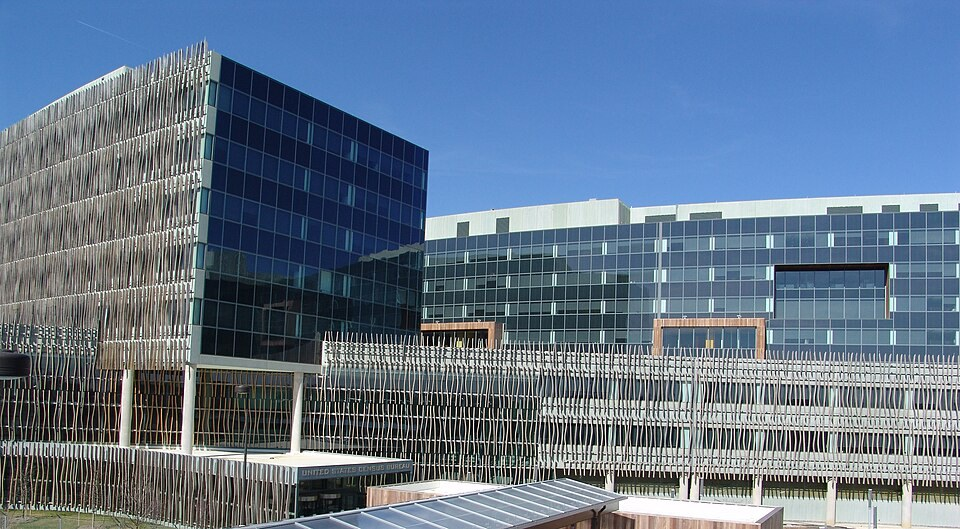
\includegraphics[height=0.24\textheight]{ch4_census_bureau_2007.jpg}\\[1mm]
\imgcap{US Census Bureau, Suitland, Maryland: the home of X-11 and X-13}
\imgcredit{https://commons.wikimedia.org/wiki/File:Census_Bureau_headquarters,_Suitland,_Maryland,_2007.jpg}{Photo: United States Census Bureau (2007); public domain; Wikimedia Commons}
\end{column}
\end{columns}
\end{frame}

\begin{frame}{Eurostat series: NSA, CA, SA, SCA}
\itemsize{\small}
\begin{itemize}
    \item Each series comes in several versions (dimension \texttt{s\_adj}):
    \begin{itemize}
        \item \textbf{NSA}: not seasonally adjusted (the raw data)
        \item \textbf{CA}: calendar adjusted only (working days, holidays)
        \item \textbf{SA}: seasonally adjusted; \textbf{SCA}: seasonally and calendar adjusted
    \end{itemize}
    \item Which one for which question
    \begin{itemize}
        \item quarter-on-quarter or month-on-month growth: SCA
        \item year-on-year growth: NSA or CA (the seasonal pattern cancels, the calendar does not)
        \item SARIMA modelling and forecasting: NSA, with calendar regressors
    \end{itemize}
    \item The annual totals of NSA and SCA are close (2024: 196.4 and 196.4 bn EUR): adjustment moves output between quarters, it does not create it
\end{itemize}
\end{frame}

\begin{frame}{Unadjusted and adjusted series}
\itemsize{\footnotesize}
\begin{center}
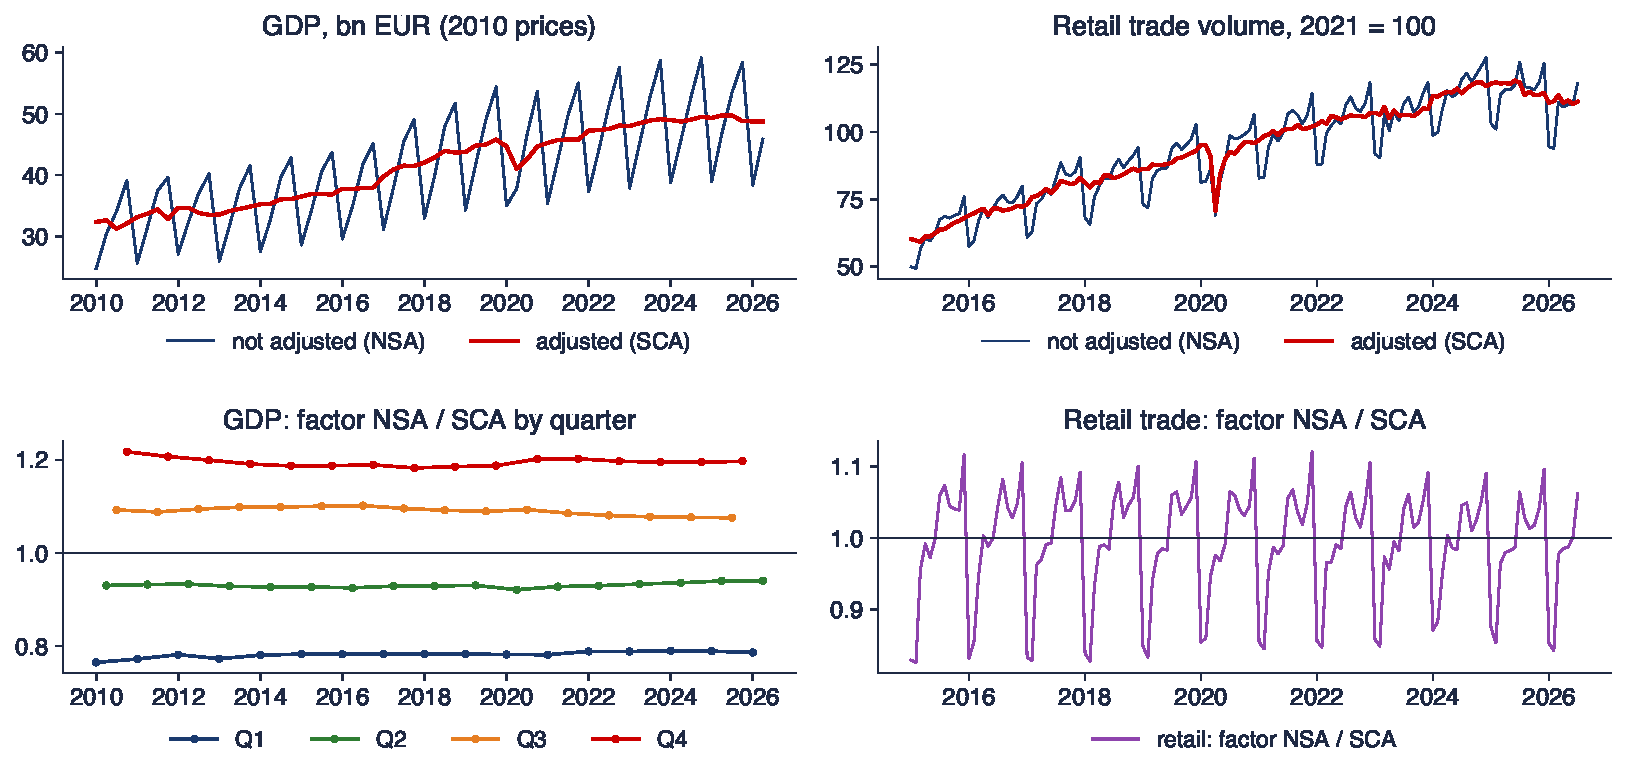
\includegraphics[width=0.97\textwidth,height=0.66\textheight,keepaspectratio]{tsa_ch4_sa_nsa.pdf}
\end{center}
\vspace{-0.25cm}
\begin{itemize}
    \item Eurostat NSA and SCA: GDP (top left) and retail trade (top right); bottom: the implied seasonal and calendar factors NSA/SCA
\end{itemize}
\quantlet{TSA\_ch4\_seasonal\_data}{\qlurl{TSA_ch4_seasonal_data}}
\end{frame}

\begin{frame}{Interpreting the adjusted series}
\itemsize{\footnotesize}
\begin{itemize}
    \item GDP factors 2015--2019: Q1 0.78, Q2 0.93, Q3 1.10, Q4 1.19: Q1 output is about a fifth below an average quarter
    \begin{itemize}
        \item the factors move slowly over the years: the stochastic seasonality that $\hat\Theta$ measures
    \end{itemize}
    \item Retail trade: December factor 1.10, January 0.84 (2016--2019): Christmas shopping, then the January low
    \item The retail factor also jumps from month to month because of working days and Easter: the calendar part of SCA (Section 7)
    \item The adjusted GDP shows the 2020 fall and the 2025--2026 stagnation that the raw series hides
\end{itemize}
\end{frame}

\begin{frame}{Recap: Seasonal adjustment}
\itemsize{\small}
\begin{itemize}
    \item Seasonal adjustment removes $\hat S_t$ and $\hat C_t$ to show the trend and the cycle
    \item X-13ARIMA-SEATS: regARIMA pre-adjustment (outliers, calendar, forecasts), then X-11 or SEATS; in the EU, JDemetra+
    \item Quarter-on-quarter growth: SCA; year-on-year growth: NSA or CA; SARIMA forecasting: NSA
\end{itemize}
\end{frame}


%=============================================================================
\section{Fourier terms and calendar effects}
%=============================================================================

\begin{frame}{Seasonal dummies and Fourier terms}
\itemsize{\small}
\begin{itemize}
    \item \textbf{Dummies}: $y_t = \beta_0 + \sum_{j=2}^{s}\gamma_jD_{jt} + u_t$: $s - 1$ coefficients, any shape
    \begin{itemize}
        \item $\beta_0$: the level of season 1; $\gamma_j$: the difference between season $j$ and season 1
        \item too many for $s = 52$ weeks, $s = 168$ hours or $s = 365$ days; impossible for $s = 365.25$
    \end{itemize}
    \item \textbf{Fourier terms} for a period $m$: $\sum_{k=1}^{K}\left[\alpha_k\sin\frac{2\pi kt}{m} + \beta_k\cos\frac{2\pi kt}{m}\right]$
    \begin{itemize}
        \item $\alpha_k, \beta_k$: the coefficients of the $k$-th harmonic, a wave with $k$ cycles per period; $K$: the number of sine--cosine pairs
        \item $2K$ coefficients; $K = m/2$ reproduces the dummies exactly (for even $m$); a small $K$ gives a smooth pattern
        \item $m$ may be non-integer, and several periods can be combined: e.g. $K = 5$ for $m = 24$ and $K = 4$ for $m = 168$ give 18 regressors instead of $23 + 167$
    \end{itemize}
    \item $K$ is chosen by AICc or by cross-validation; the same terms are inside TBATS and Prophet (Section 9)
\end{itemize}
\end{frame}

\begin{frame}{Fourier approximation of a seasonal pattern}
\itemsize{\footnotesize}
\begin{center}
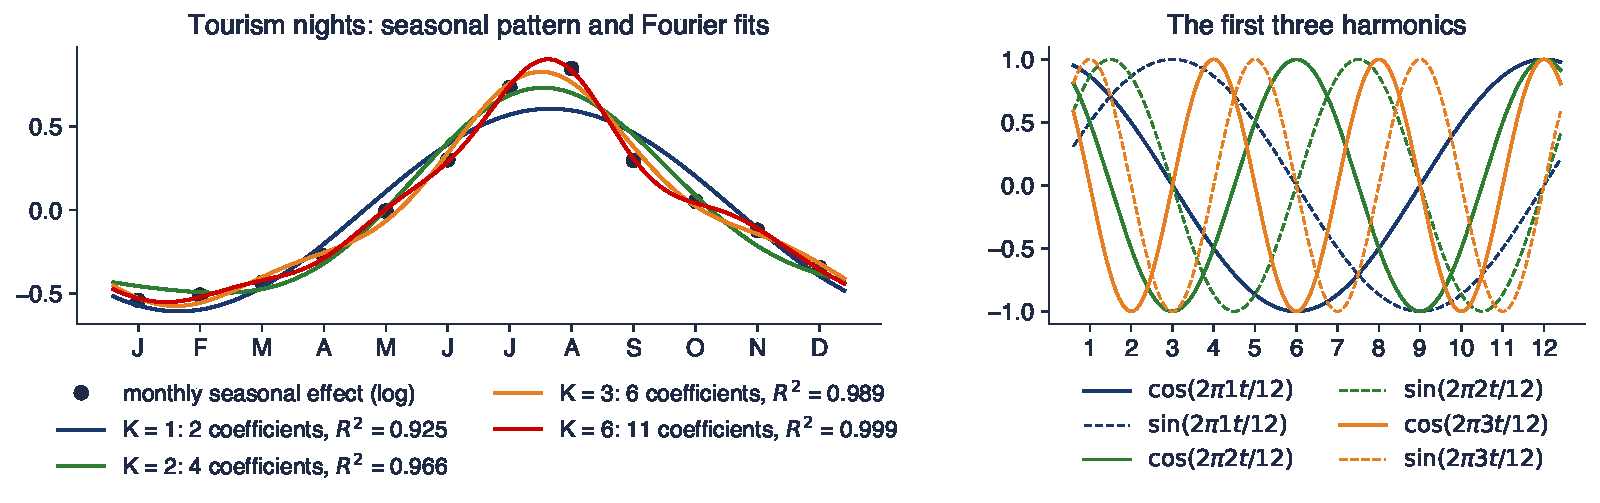
\includegraphics[width=0.97\textwidth,height=0.58\textheight,keepaspectratio]{tsa_ch4_fourier.pdf}
\end{center}
\vspace{-0.25cm}
\begin{itemize}
    \item Monthly seasonal effect of $\ln$(tourism nights), 2012--2019, after removing a 13-month centred mean; fits with $K = 1, 2, 3, 6$
\end{itemize}
\quantlet{TSA\_ch4\_calendar\_fourier}{\qlurl{TSA_ch4_calendar_fourier}}
\end{frame}

\begin{frame}{Interpreting the Fourier fits}
\itemsize{\small}
\begin{itemize}
    \item $K = 1$ (two coefficients) already gives $R^2 = 0.925$: the summer peak is close to a single wave
    \begin{itemize}
        \item $K = 2$: 0.966; $K = 3$: 0.989 with six coefficients instead of eleven
    \end{itemize}
    \item $K = 6$ (11 coefficients) interpolates the 12 monthly points: the same as 11 dummies, $R^2 = 0.999$
    \item Higher harmonics add sharper detail: the August peak needs $K \ge 3$
\end{itemize}
\end{frame}

\begin{frame}{Calendar effects and Orthodox Easter}
\itemsize{\footnotesize}
\begin{columns}[T]
\begin{column}{0.66\textwidth}
\begin{itemize}
    \item \textbf{Working days}: a month with more Monday--Friday non-holiday days produces and sells more
    \begin{itemize}
        \item known in advance: a regressor that can be used in forecasts
    \end{itemize}
    \item \textbf{Moving holidays}: Orthodox Easter falls between 4 April and 8 May
    \begin{itemize}
        \item 5 May 2024, 20 April 2025, 12 April 2026, 2 May 2027: shopping shifts between March, April and May
        \item in Python: \texttt{dateutil.easter.easter(y, EASTER\_ORTHODOX)}; Pentecost is 49 days later
    \end{itemize}
    \item \textbf{Easter regressor} (X-13 \texttt{easter[w]}): $E_t$ = share of the $w$ days before Easter Sunday that fall in month $t$
    \begin{itemize}
        \item $w = 10$: Easter on 20 April gives $E_{\text{April}} = 1$; on 5 May, $E_{\text{April}} = 0.6$ and $E_{\text{May}} = 0.4$
    \end{itemize}
\end{itemize}
\end{column}
\begin{column}{0.30\textwidth}
\centering

\includegraphics[height=0.26\textheight]{ch4_romanian_easter_eggs.jpg}\\[1mm]
\imgcap{Painted Easter eggs from Romania}
\imgcredit{https://commons.wikimedia.org/wiki/File:Painted_Romanian_Easter_Eggs.jpg}{Photo: jackmac34 (Pixabay); CC0; Wikimedia Commons}
\end{column}
\end{columns}
\end{frame}

\begin{frame}{Regression with SARIMA errors}
\itemsize{\small}
\begin{itemize}
    \item $100\ln y_t = \beta_EE_t + \beta_W\,\mathrm{WD}_t + \text{outlier dummies} + u_t$, with $u_t \sim$ SARIMA$(0,1,1)(0,1,1)_{12}$
    \begin{itemize}
        \item $E_t$: the Easter regressor; $\mathrm{WD}_t$: the number of working days in month $t$; $\beta_E$, $\beta_W$: their effects, in \%
        \item the ``regARIMA'' model of X-13; estimated in one step by maximum likelihood (\texttt{SARIMAX} with \texttt{exog})
        \item ordinary least squares with SARIMA errors ignored would give wrong standard errors (\tsachlink{https://danpele.github.io/Time-Series-Analysis/EN/Courses/chapter3_unit_roots_arima_models.pdf}{Chapter 3}, spurious regression)
    \end{itemize}
    \item Data: Eurostat retail trade volume, Romania, not adjusted, January 2010--July 2026: food (G47\_FOOD) and all retail (G47)
    \begin{itemize}
        \item dummies for April and May 2020 (lockdown)
    \end{itemize}
\end{itemize}
\end{frame}

\begin{frame}{Easter and Romanian retail trade}
\itemsize{\footnotesize}
\begin{center}
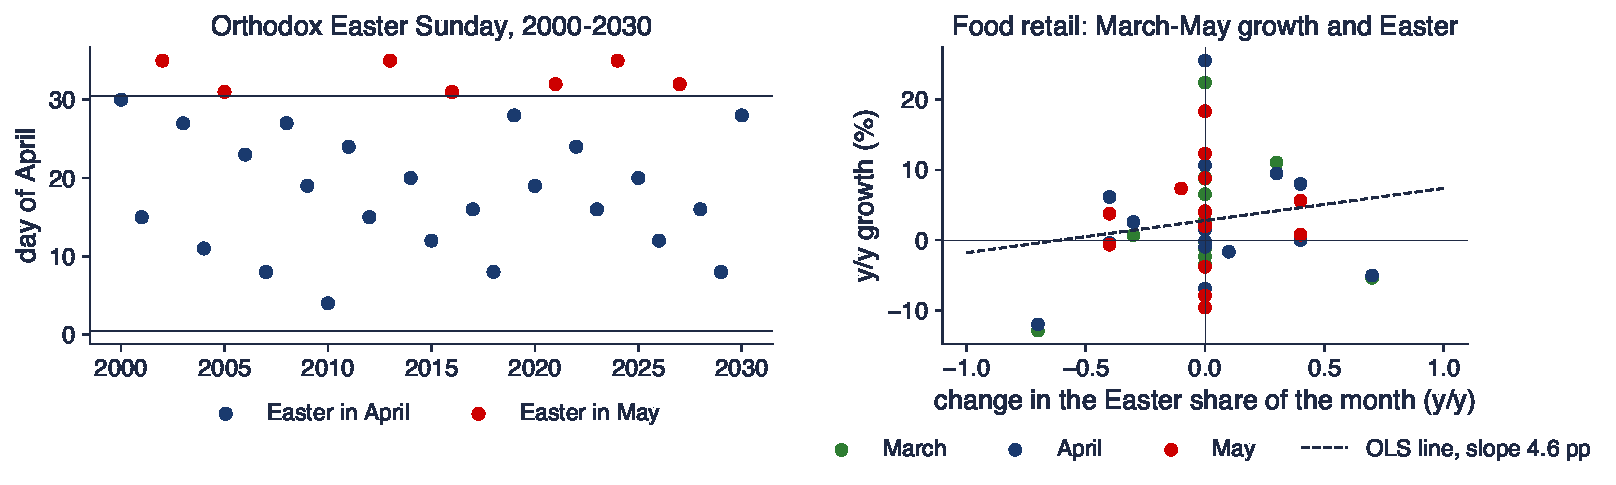
\includegraphics[width=0.97\textwidth,height=0.56\textheight,keepaspectratio]{tsa_ch4_easter.pdf}
\end{center}
\vspace{-0.25cm}
\begin{itemize}
    \item Left: Orthodox Easter Sunday as a day of April (above 30: May); right: year-on-year growth of food retail in March--May against the change in the Easter share (2020--2021 left out)
\end{itemize}
\quantlet{TSA\_ch4\_calendar\_fourier}{\qlurl{TSA_ch4_calendar_fourier}}
\end{frame}

\begin{frame}{Interpreting the Easter effect}
\itemsize{\footnotesize}
\begin{itemize}
    \item Food retail: $\hat\beta_E = 5.9\%$ (se 2.3, $t = 2.6$): a month that holds the 10 days before Easter sells about 5.9\% more food
    \begin{itemize}
        \item one working day more: $+0.59\%$ (se 0.17); April 2020: $\ensuremath{-}15\%$
    \end{itemize}
    \item All retail: Easter $0.8\%$ (se 1.9), not significant; working days $+1.02\%$ (se 0.15)
    \begin{itemize}
        \item the Easter effect is in food, the working-day effect in everything
    \end{itemize}
    \item The raw scatter is noisy (slope 4.6 percentage points): VAT changes and prices also move year-on-year growth; the regression separates the effects
    \item Easter fell in May in 2002, 2005, 2013, 2016, 2021, 2024: a forecaster who ignores this mistakes April and May
\end{itemize}
\end{frame}

\begin{frame}{Recap: Fourier terms and calendar effects}
\itemsize{\small}
\begin{itemize}
    \item Fourier terms describe a seasonal pattern with $2K$ coefficients, for any period, even non-integer
    \item Working days and moving holidays are known in advance: model them as regressors
    \item Romanian food retail rises about 5.9\% in the Easter month; total retail follows working days
    \item Regression with SARIMA errors: estimate regressors and dynamics together
\end{itemize}
\end{frame}


%=============================================================================
\section{Multiple seasonality: electricity load}
%=============================================================================

\begin{frame}{Electricity load in Romania}
\itemsize{\footnotesize}
\begin{columns}[T]
\begin{column}{0.60\textwidth}
\begin{itemize}
    \item \textbf{Load}: the electricity consumed in the system, in MW (hourly averages); it must be matched by generation at every moment
    \begin{itemize}
        \item forecasts are needed for every hour of the next day: day-ahead markets, reserves, grid planning
    \end{itemize}
    \item Data: ENTSO-E (the European network of transmission system operators), ``monthly hourly load values'', Romania
    \begin{itemize}
        \item 39\,406 hours, 2022--2026, Romanian winter time (UTC+2) to avoid the clock changes
    \end{itemize}
    \item Load forecasting has its own competitions: GEFCom2014 (\refGEF)
\end{itemize}
\end{column}
\begin{column}{0.36\textwidth}
\centering
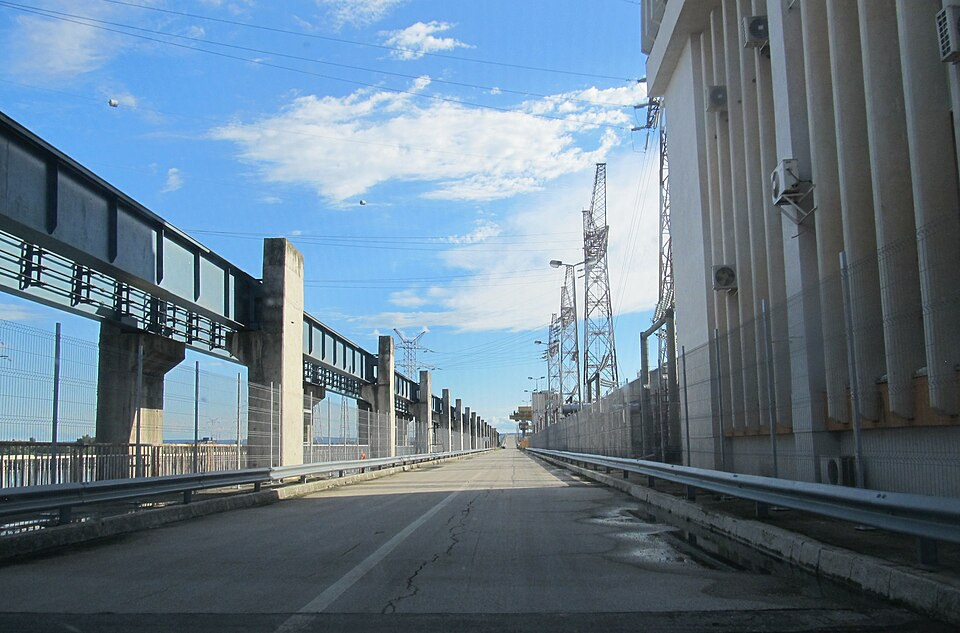
\includegraphics[height=0.30\textheight]{ch4_portile_de_fier_ii.jpg}\\[1mm]
\imgcap{Iron Gates II hydropower plant on the Danube}
\imgcredit{https://commons.wikimedia.org/wiki/File:Por\%C8\%9Bile_de_Fier_II_(01).jpg}{Photo: Nenea hartia (2016); CC BY-SA 4.0; Wikimedia Commons}
\end{column}
\end{columns}
\end{frame}

\begin{frame}{Hourly load: the day and the week}
\itemsize{\footnotesize}
\begin{center}
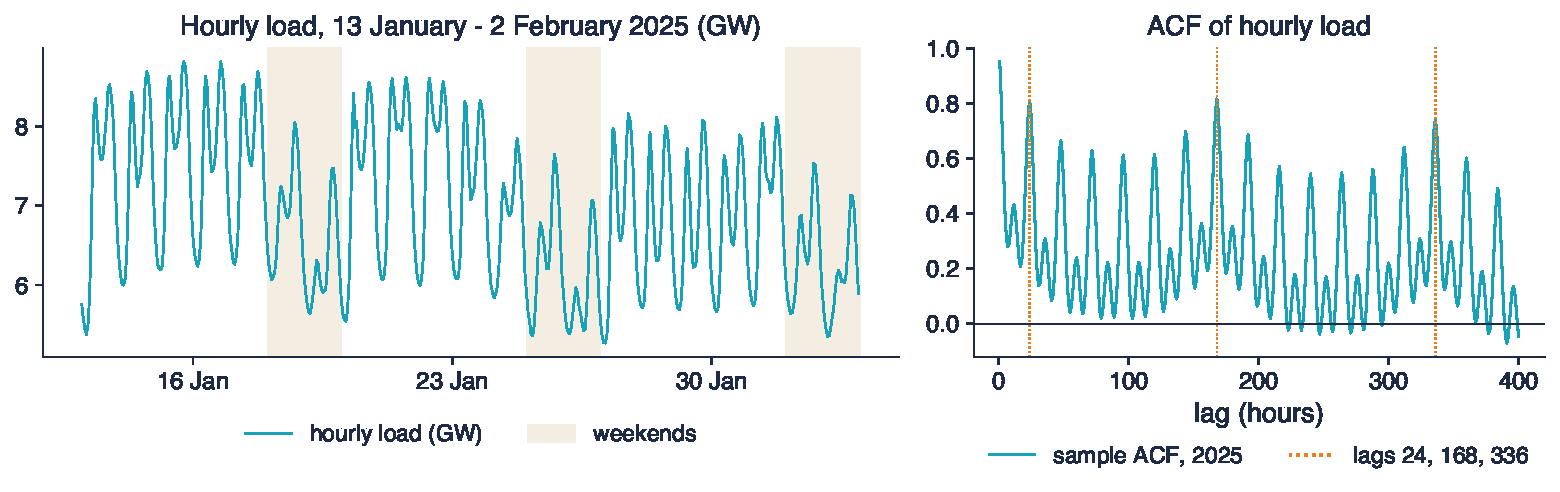
\includegraphics[width=0.97\textwidth,height=0.56\textheight,keepaspectratio]{tsa_ch4_load_hourly.pdf}
\end{center}
\vspace{-0.25cm}
\begin{itemize}
    \item Left: three weeks of January 2025; right: sample ACF of all hours of 2025 up to lag 400
\end{itemize}
\quantlet{TSA\_ch4\_multiple\_seasonality}{\qlurl{TSA_ch4_multiple_seasonality}}
\end{frame}

\begin{frame}{Interpreting the hourly load}
\itemsize{\footnotesize}
\begin{itemize}
    \item Daily cycle: lowest around 3:00 (5.3 GW on average in 2025), highest around 19:00 (7.3 GW)
    \begin{itemize}
        \item ACF $0.81$ at lag 24, $0.43$ at lag 12
    \end{itemize}
    \item Weekly cycle: weekends are lower; ACF $0.82$ at lag 168 (one week), above the lag-24 value
    \begin{itemize}
        \item the same hour one week ago is the best single predictor: Monday is like last Monday, not like Sunday
    \end{itemize}
    \item And an annual cycle on top (heating and air conditioning): three periods, 24, 168 and about 8766 hours
    \item SARIMA is not enough: it has one integer period $s$, while here $s = 24$, $168$ and $8766$ act at once
    \begin{itemize}
        \item a polynomial in $L^{168}$ is slow and unstable, 365.25 is not an integer, and holidays break the weekly pattern
        \item answers: MSTL, the dynamic harmonic regression (DHR), TBATS, Prophet
    \end{itemize}
\end{itemize}
\end{frame}

\begin{frame}{MSTL: one seasonal component per period}
\itemsize{\footnotesize}
\begin{center}
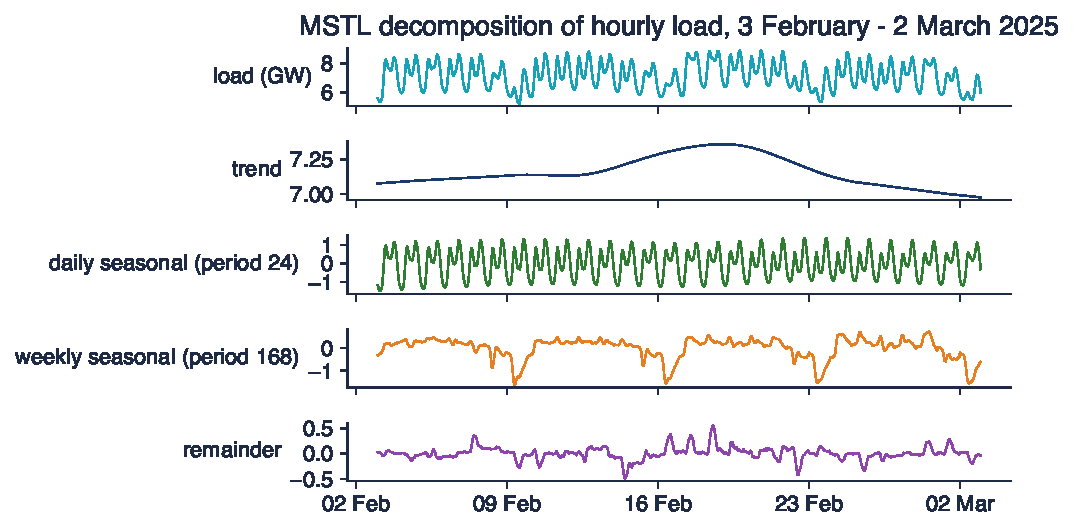
\includegraphics[width=0.97\textwidth,height=0.64\textheight,keepaspectratio]{tsa_ch4_mstl.pdf}
\end{center}
\vspace{-0.25cm}
\begin{itemize}
    \item MSTL (\refMSTL) applies STL (\tsachlink{https://danpele.github.io/Time-Series-Analysis/EN/Courses/chapter0_introduction.pdf}{Chapter 0}) repeatedly, once for each period (24 and 168 hours), until the components settle
\end{itemize}
\quantlet{TSA\_ch4\_multiple\_seasonality}{\qlurl{TSA_ch4_multiple_seasonality}}
\end{frame}

\begin{frame}{Interpreting the MSTL decomposition}
\itemsize{\small}
\begin{itemize}
    \item Of the variance around the trend: 70\% daily component, 29\% weekly component, 2\% remainder
    \begin{itemize}
        \item range of the daily component in the first week: 2.8 GW; of the weekly one: 2.1 GW
    \end{itemize}
    \item The weekly component is flat Monday to Friday and drops on Saturday and more on Sunday
    \item The remainder is small but not white noise: cold spells and holidays; a forecasting model adds dynamics and regressors
\end{itemize}
\end{frame}

\begin{frame}{Daily load and public holidays}
\itemsize{\footnotesize}
\begin{center}
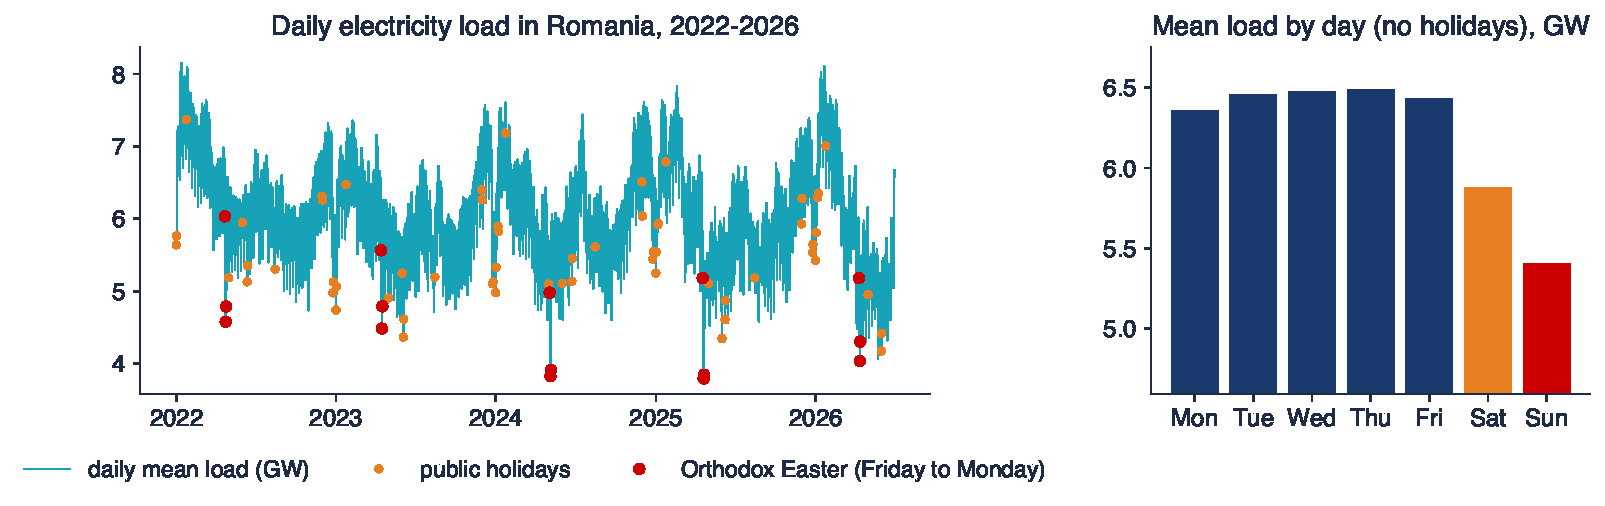
\includegraphics[width=0.97\textwidth,height=0.56\textheight,keepaspectratio]{tsa_ch4_load_daily.pdf}
\end{center}
\vspace{-0.25cm}
\begin{itemize}
    \item Daily mean load, 2022--2026, 1\,642 days; Romanian public holidays marked; right: mean by day of the week, holidays excluded
\end{itemize}
\quantlet{TSA\_ch4\_multiple\_seasonality}{\qlurl{TSA_ch4_multiple_seasonality}}
\end{frame}

\begin{frame}{Interpreting the daily load}
\itemsize{\small}
\begin{itemize}
    \item Week: Saturday 9\% and Sunday 17\% below Wednesday
    \begin{itemize}
        \item Year: January 25\% above May; a smaller summer peak (air conditioning)
    \end{itemize}
    \item Holidays: the lowest day of the sample is Easter Sunday, 20 April 2025 (3.79 GW, mean 6.18 GW)
    \begin{itemize}
        \item the four Easter days (Friday to Monday) average 4.62 GW; Christmas to New Year is also low
    \end{itemize}
    \item The level falls over 2022--2026; possible causes: the price shock of 2022 and rooftop solar panels that cover part of the demand behind the meter
\end{itemize}
\end{frame}

\begin{frame}{A dynamic harmonic regression for daily load}
\itemsize{\footnotesize}
\begin{itemize}
    \item $y_t = \sum_{k=1}^{4}\left[\alpha_k\sin\frac{2\pi kt}{365.25} + \beta_k\cos\frac{2\pi kt}{365.25}\right] + \sum_{j}\delta_jD^{\mathrm{day}}_{jt} + \lambda_1H_t + \lambda_2E_t + \lambda_3X_t + u_t$
    \begin{itemize}
        \item $\alpha_k, \beta_k$: annual Fourier coefficients; $\delta_j$: effect of weekday $j$ against Sunday; $\lambda_1, \lambda_2, \lambda_3$: effects of the special days, in GW
        \item annual Fourier terms; weekday dummies (Sunday is the base); $H$ public holiday, $E$ Easter (Friday to Monday), $X$ 24 December -- 2 January
        \item $u_t \sim$ ARIMA(1,1,1), chosen by AIC: \textbf{dynamic harmonic regression} (DHR, \refFPPdhr)
    \end{itemize}
    \item Estimates, data to the first forecast origin (30 June 2025), in GW:
    \begin{itemize}
        \item Wednesday $+1.08$, Monday $+0.88$, Saturday $+0.50$ relative to Sunday
        \item public holiday $-0.38$ (se 0.02), Easter $-0.58$ more, Christmas--New Year $-0.61$
        \item errors: AR $0.80$, MA $\ensuremath{-}0.98$, $\hat\sigma = 186$ MW; Ljung--Box(14) p $<$\,0.001: some dynamics left
    \end{itemize}
\end{itemize}
\end{frame}

\begin{frame}{Recap: Multiple seasonality}
\itemsize{\small}
\begin{itemize}
    \item Hourly load has daily, weekly and annual cycles; daily load has weekly and annual cycles
    \item SARIMA handles one integer period; MSTL decomposes several
    \item Holidays, Easter most of all, are the largest deviations: they need regressors
    \item DHR = Fourier terms + calendar dummies + ARIMA errors: flexible and transparent
\end{itemize}
\end{frame}


%=============================================================================
\section{TBATS and Prophet}
%=============================================================================

\begin{frame}{TBATS}
\itemsize{\footnotesize}
\begin{itemize}
    \item \refTBATS: exponential smoothing (ETS, \tsachlink{https://danpele.github.io/Time-Series-Analysis/EN/Courses/chapter0_introduction.pdf}{Chapter 0}) for complex seasonality; the name lists its parts
    \begin{itemize}
        \item trigonometric seasonality (T), Box--Cox transformation (B), ARMA errors (A), trend (T), seasonal components (S)
    \end{itemize}
    \item $y_t^{(\omega)} = \ell_{t-1} + \phi b_{t-1} + \sum_{i}s^{(i)}_{t-1} + d_t$, $d_t$ ARMA($p,q$); level and trend updated as in Holt's method
    \begin{itemize}
        \item $y_t^{(\omega)}$: the series after a Box--Cox transformation with parameter $\omega$; $\ell_t$: level; $b_t$: slope; $\phi$: damping factor; $s^{(i)}_t$: seasonal component $i$
        \item each period $m_i$ has $K_i$ harmonics $s^{(i)}_{j,t}$, each a rotating pair (cosine, sine) updated by the errors: a Fourier pattern that can evolve
    \end{itemize}
    \item Automatic choices by AIC: Box--Cox or not, trend or damped trend or none, the $K_i$, the ARMA orders
    \begin{itemize}
        \item daily load to June 2025, periods 7 and 365.25 (no Box--Cox, no trend): $K = 3$ weekly and $K = 9$ annual harmonics, ARMA(1,2), 28 states
    \end{itemize}
    \item Limits: no regressors, hence no holidays or Easter; slow on long series; Python package \texttt{tbats}
\end{itemize}
\end{frame}

\begin{frame}{Prophet}
\itemsize{\footnotesize}
\begin{itemize}
    \item \refProphet{} (Meta): a regression in time, $y(t) = g(t) + s(t) + h(t) + \varepsilon_t$
    \begin{itemize}
        \item $g(t)$: piecewise-linear (or logistic) trend whose slope may change at \textbf{changepoints}; a Laplace prior shrinks most changes to zero
        \item $s(t)$: Fourier terms, by default $K = 10$ for the year and $K = 3$ for the week
        \item $h(t)$: one effect per holiday (with optional windows around it), from a list of dates
    \end{itemize}
    \item Estimated by Stan (maximum a posteriori); intervals simulate future changepoints and the noise
    \begin{itemize}
        \item no autoregressive part: today's surprise does not move tomorrow's forecast
    \end{itemize}
    \item Built for many business series with strong calendar effects and missing data; Python package \texttt{prophet}
\end{itemize}
\end{frame}

\begin{frame}{Prophet components for daily load}
\itemsize{\footnotesize}
\begin{center}
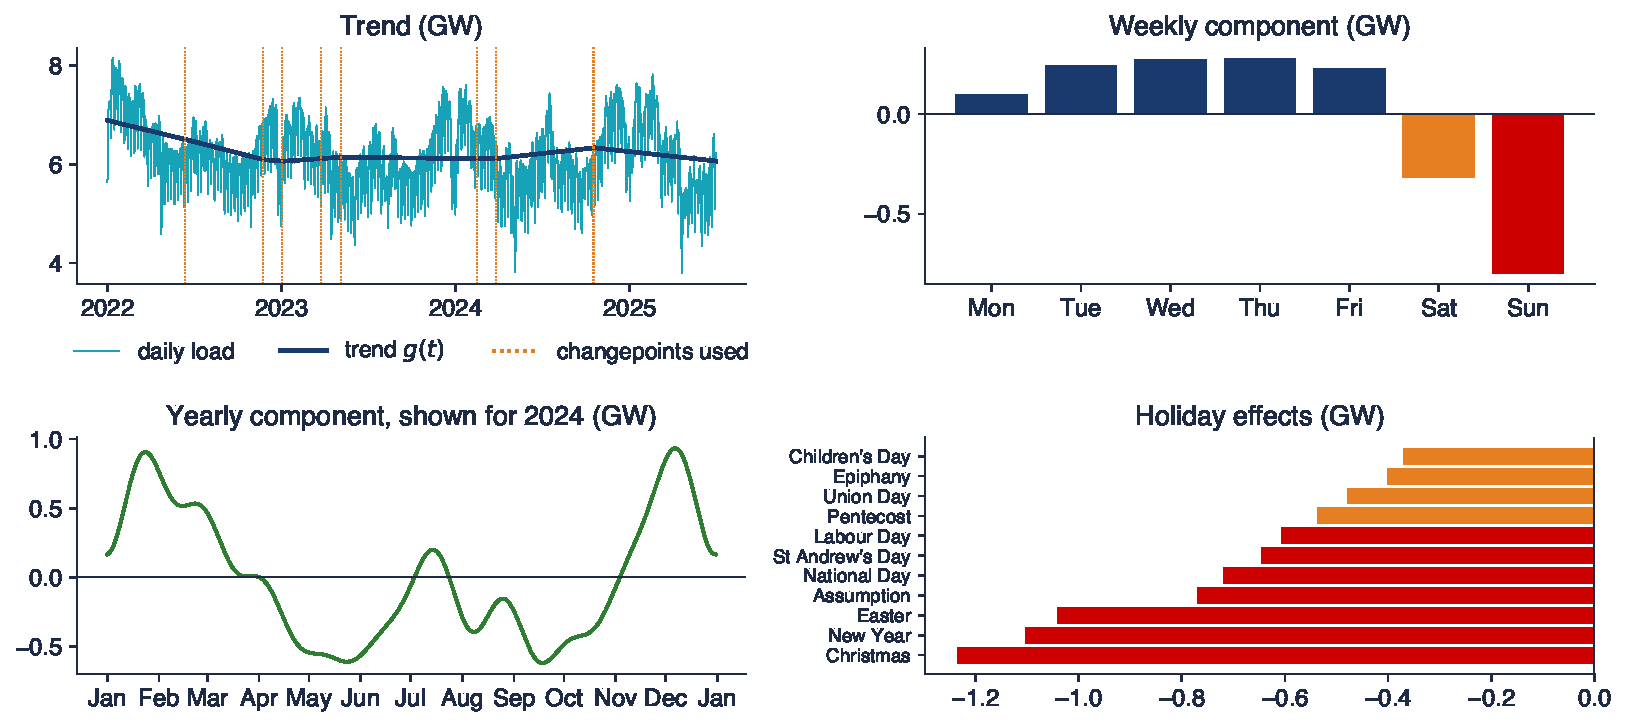
\includegraphics[width=0.97\textwidth,height=0.64\textheight,keepaspectratio]{tsa_ch4_prophet.pdf}
\end{center}
\vspace{-0.25cm}
\begin{itemize}
    \item Prophet with Romanian public holidays, daily load 2022 -- June 2025
\end{itemize}
\quantlet{TSA\_ch4\_tbats\_prophet}{\qlurl{TSA_ch4_tbats_prophet}}
\end{frame}

\begin{frame}{Interpreting the Prophet components}
\itemsize{\small}
\begin{itemize}
    \item Trend from 6.89 to 6.07 GW, flatter after 2023; 25 candidate changepoints, most shrunk to zero
    \begin{itemize}
        \item weekly: Wednesday $+0.27$, Saturday $\ensuremath{-}0.32$, Sunday $\ensuremath{-}0.80$ GW
    \end{itemize}
    \item Yearly: highest in early December ($+0.93$ GW, 7 December 2024), lowest in mid-September ($\ensuremath{-}0.62$ GW, 18 September 2024), shown for 2024
    \item Holidays: Christmas $\ensuremath{-}1.24$, New Year $\ensuremath{-}1.10$, Easter $\ensuremath{-}1.04$ GW; Children's Day only $\ensuremath{-}0.37$ GW
    \item Each component is readable and can be checked against what we know about the economy
\end{itemize}
\end{frame}

\begin{frame}{Recap: DHR, TBATS and Prophet side by side}
\itemsize{\footnotesize}
\begin{center}
\scriptsize
\begin{tabular}{>{\raggedright\arraybackslash}p{2.6cm}>{\raggedright\arraybackslash}p{2.8cm}>{\raggedright\arraybackslash}p{2.8cm}>{\raggedright\arraybackslash}p{2.8cm}}
\toprule
 & \textbf{DHR} & \textbf{TBATS} & \textbf{Prophet} \\
\midrule
Seasonality & Fourier, fixed & Fourier, evolving & Fourier, fixed \\
Several periods & yes & yes & yes \\
Holidays, regressors & yes & no & yes \\
Short-run dynamics & ARMA errors & ARMA errors & none \\
Trend & through the errors (ARIMA) & local (Holt) & piecewise linear \\
Speed & fast & slow & fast \\
\bottomrule
\end{tabular}
\end{center}
\begin{itemize}
    \item All three are regressions on sines and cosines at heart; they differ in what else they model
    \item Which forecasts best is an empirical question: the next section answers it out of sample
\end{itemize}
\end{frame}


%=============================================================================
\section{Forecast evaluation}
%=============================================================================

\begin{frame}{Time-series cross-validation}
\itemsize{\footnotesize}
\begin{center}
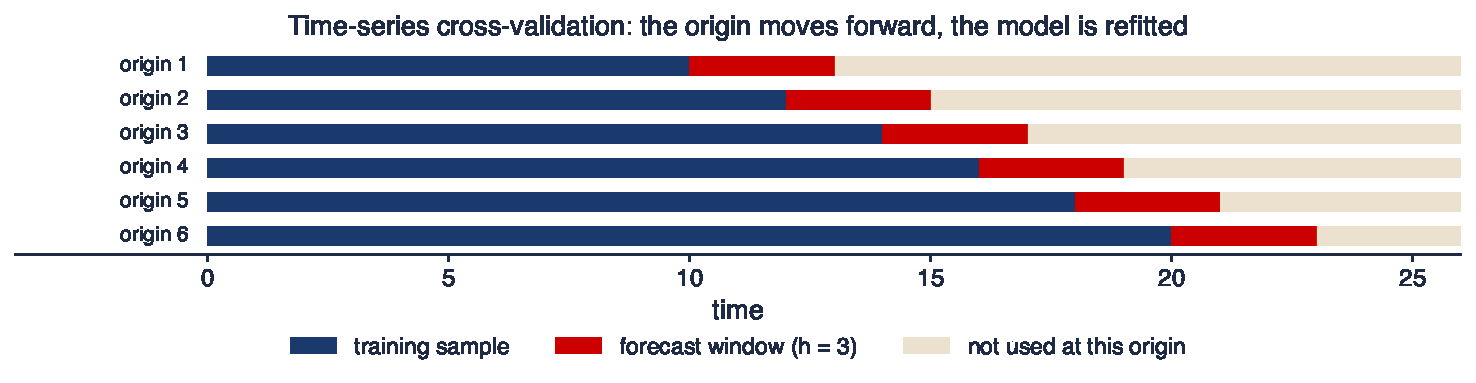
\includegraphics[width=0.97\textwidth,height=0.40\textheight,keepaspectratio]{tsa_ch4_cv_scheme.pdf}
\end{center}
\vspace{-0.25cm}
\begin{itemize}
    \item Rolling forecast origin (\refTashman; \refFPPcv): fit on the data up to the origin, forecast $h$ steps, move the origin, refit
    \item Expanding window (shown) or sliding window of fixed length; never use future data to fit
\end{itemize}
\quantlet{TSA\_ch4\_evaluation}{\qlurl{TSA_ch4_evaluation}}
\end{frame}

\begin{frame}{Interpreting the design of our experiment}
\itemsize{\footnotesize}
\begin{itemize}
    \item Daily load: 26 origins every 14 days, from 30 June 2025 to 15 June 2026; horizon $h = 14$ days
    \begin{itemize}
        \item one year of out-of-sample forecasts, every season and every holiday, Easter 2026 included
    \end{itemize}
    \item Seven methods, all refitted at each origin
    \begin{itemize}
        \item seasonal naive (period 7); ETS (Holt--Winters, damped trend, period 7); SARIMA(2,0,1)$(0,1,1)_7$; DHR; TBATS; Prophet
        \item Combination: the simple average of the five model forecasts (all except the seasonal naive)
    \end{itemize}
    \item The orders of SARIMA and of the DHR errors are chosen once, by AIC, on the data before the first origin: no peeking at the test period
    \item Cross-validation that ignores time order (random folds) is valid only for pure autoregressions with white-noise errors (\refBHK)
\end{itemize}
\end{frame}

\begin{frame}{The Diebold--Mariano test}
\itemsize{\footnotesize}
\begin{itemize}
    \item \refDM: is the difference in accuracy between two forecasts larger than chance?
    \begin{itemize}
        \item $e_{1t}$, $e_{2t}$: the errors of the two forecasts; $L$: the loss function
        \item loss differential $d_t = L(e_{1t}) - L(e_{2t})$, $L(e) = e^2$ or $|e|$; $H_0$: $E[d_t] = 0$
    \end{itemize}
    \item $\mathrm{DM} = \dfrac{\bar d}{\sqrt{\hat V/n}}$, $\hat V = \hat\gamma_d(0) + 2\sum_{k=1}^{h-1}\hat\gamma_d(k)$
    \begin{itemize}
        \item $\bar d$: the mean of the $n$ differentials; $\hat\gamma_d(k)$: their autocovariance at lag $k$; a negative DM favours forecast 1
        \item $h$-step errors overlap, so $d_t$ is autocorrelated up to lag $h - 1$
        \item asymptotically $N(0, 1)$; small samples: $\mathrm{HLN} = \sqrt{\frac{n + 1 - 2h + h(h - 1)/n}{n}}\;\mathrm{DM}$, compared with $t(n - 1)$ (\refHLN)
    \end{itemize}
    \item Our design: one value per origin, $d_j$ = average loss difference over the 14-day window; the windows do not overlap, so $h = 1$ in the formula
    \begin{itemize}
        \item the test compares forecasts, not models: re-estimation noise is part of what is tested
    \end{itemize}
\end{itemize}
\end{frame}

\begin{frame}{Worked example: a Diebold--Mariano test}
\itemsize{\small}
\begin{itemize}
    \item Five windows; window-average differences in squared error, method 1 minus method 2: $-0.30, 0.10, -0.50, -0.20, -0.40$
    \begin{itemize}
        \item $\bar d = \ensuremath{-}0.26$: method 1 has the smaller losses in four windows out of five
    \end{itemize}
    \item $\hat\gamma_d(0) = \frac15\sum(d_j - \bar d)^2 = 0.042$
    \begin{itemize}
        \item $\mathrm{DM} = \ensuremath{-}0.26/\sqrt{0.042/5} = \ensuremath{-}2.82$; $\mathrm{HLN} = \sqrt{4/5}\cdot\mathrm{DM} = \ensuremath{-}2.53$
    \end{itemize}
    \item $|\ensuremath{-}2.53| < t_{0.975}(4) = 2.78$ (p = 0.065): equal accuracy is not rejected at 5\%
    \begin{itemize}
        \item the normal critical value 1.96 would have rejected: with few windows, the correction matters
    \end{itemize}
\end{itemize}
\end{frame}

\begin{frame}{Forecasts from one origin, across Easter 2026}
\itemsize{\footnotesize}
\begin{center}
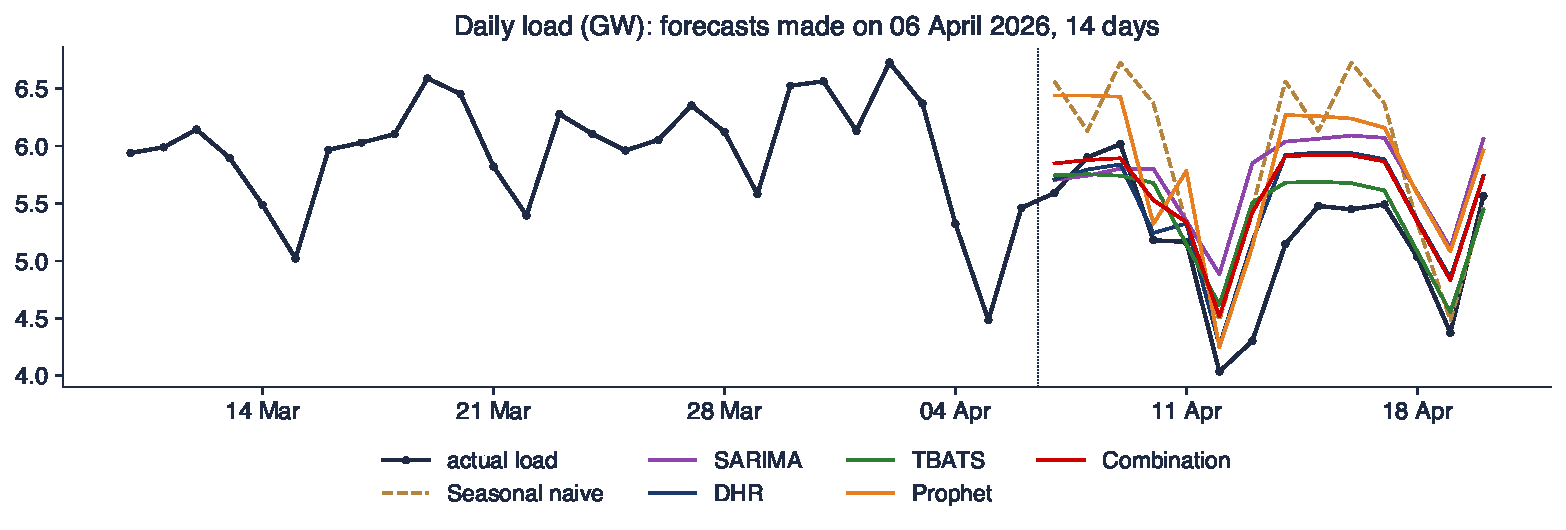
\includegraphics[width=0.97\textwidth,height=0.56\textheight,keepaspectratio]{tsa_ch4_load_fc.pdf}
\end{center}
\vspace{-0.25cm}
\begin{itemize}
    \item Origin 6 April 2026, 14 days ahead; Orthodox Easter Sunday was 12 April 2026
\end{itemize}
\quantlet{TSA\_ch4\_evaluation}{\qlurl{TSA_ch4_evaluation}}
\end{frame}

\begin{frame}{Interpreting one forecast window}
\itemsize{\small}
\begin{itemize}
    \item MAE in this window (MW): ETS 299, TBATS 309, DHR 344, Combination 394, SARIMA 584, Prophet 616, seasonal naive 686
    \begin{itemize}
        \item the seasonal naive method copies the previous normal week into Easter week
    \end{itemize}
    \item Every model sees the Sunday dip; DHR and Prophet also lower Good Friday and Easter Monday, which the weekly models treat as working days
    \item After Easter the load stays below every forecast for the rest of the week; ETS and TBATS, whose level follows the latest days, lose least here
    \item One window is anecdote; the next slides average over all 26 windows
\end{itemize}
\end{frame}

\begin{frame}{Cross-validation results for daily load}
\itemsize{\footnotesize}
\begin{center}
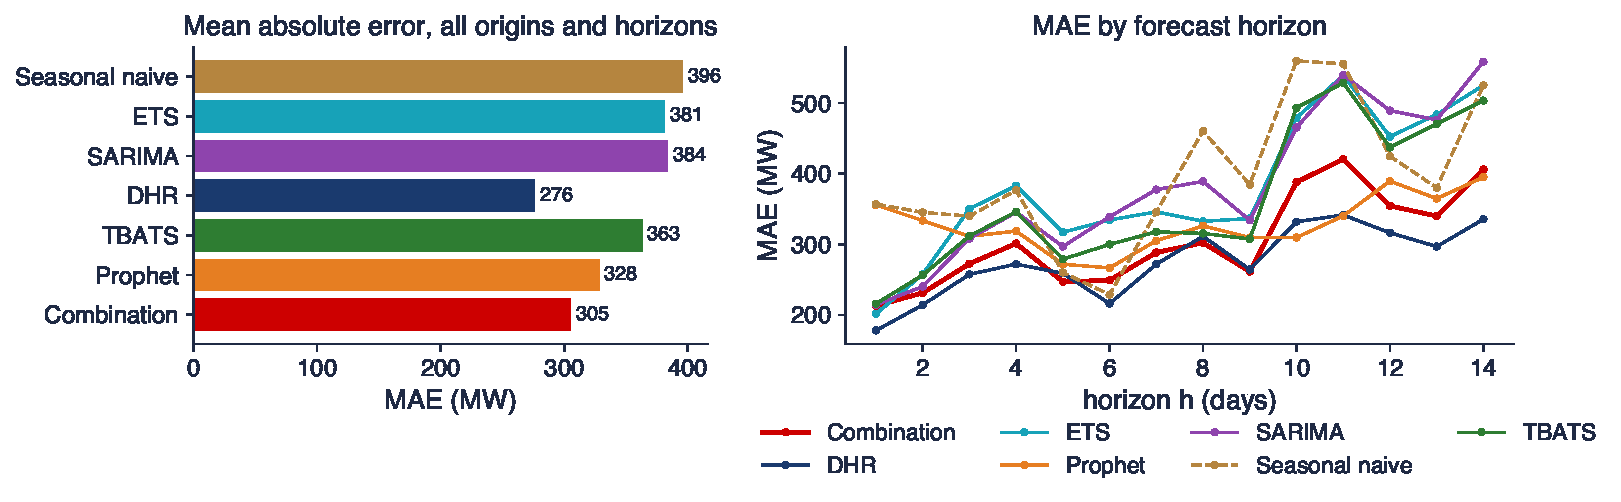
\includegraphics[width=0.97\textwidth,height=0.56\textheight,keepaspectratio]{tsa_ch4_cv_results.pdf}
\end{center}
\vspace{-0.25cm}
\begin{itemize}
    \item 26 origins $\times$ 14 horizons for each method; left: overall MAE; right: MAE by horizon
\end{itemize}
\quantlet{TSA\_ch4\_evaluation}{\qlurl{TSA_ch4_evaluation}}
\end{frame}

\begin{frame}{Interpreting the cross-validation results}
\itemsize{\footnotesize}
\begin{center}
\scriptsize
\begin{tabular}{lrrrrr}
\toprule
\textbf{Method} & \textbf{MAE} & \textbf{RMSE} & \textbf{MASE} & \textbf{DM against s. naive} & \textbf{DM against DHR} \\
\midrule
Seasonal naive & 396 & 529 & 1.28 & -- & $4.42$ ($<$\,0.001) \\
ETS & 381 & 492 & 1.23 & $\ensuremath{-}0.80$ (0.431) & $3.08$ (0.005) \\
SARIMA & 384 & 477 & 1.24 & $\ensuremath{-}1.23$ (0.231) & $3.29$ (0.003) \\
DHR & \textbf{276} & \textbf{350} & \textbf{0.89} & $\ensuremath{-}4.42$ ($<$\,0.001) & -- \\
TBATS & 363 & 468 & 1.18 & $\ensuremath{-}1.50$ (0.145) & $3.02$ (0.006) \\
Prophet & 328 & 412 & 1.06 & $\ensuremath{-}2.99$ (0.006) & $2.76$ (0.011) \\
Combination & 305 & 380 & 0.99 & $\ensuremath{-}3.82$ ($<$\,0.001) & $1.89$ (0.070) \\
\bottomrule
\end{tabular}
\end{center}
\begin{itemize}
    \item MAE and RMSE in MW; MASE (\refHKo) = MAE / 309 MW, the in-sample MAE of the weekly seasonal naive method; DM: HLN statistic (p-value) on window-average squared errors, row method minus column method
    \item DHR wins; with the combination, it is the only method with MASE below 1; Prophet is the second single model: the two that know the holidays
    \item ETS, SARIMA and TBATS are not significantly better than the seasonal naive method
\end{itemize}
\end{frame}

\begin{frame}{A second test: Romanian GDP}
\itemsize{\footnotesize}
\begin{center}
\scriptsize
\begin{tabular}{lrrrr}
\toprule
\textbf{Method} & MAE, $h = 1$ & MAE, $h = 4$ & without 2019--2020, $h = 1$ & without 2019--2020, $h = 4$ \\
\midrule
SARIMA (airline) & 1.69 & 2.70 & 1.32 & 1.89 \\
ETS & 1.76 & 2.84 & 1.41 & 2.44 \\
Seasonal naive & 3.81 & 3.74 & 3.80 & 3.49 \\
Combination (SARIMA, ETS) & 1.70 & 2.65 & 1.34 & 2.02 \\
\bottomrule
\end{tabular}
\end{center}
\begin{itemize}
    \item $100\ln Y$, errors in \%; 51 quarterly origins, 2012Q4--2025Q2, expanding window; 43 origins without 2019--2020
    \item DM (HLN), SARIMA against ETS: $h = 1$: $\ensuremath{-}1.46$ (p = 0.150); $h = 4$: $0.50$ (p = 0.620)
    \item SARIMA against the seasonal naive method: $h = 1$: $\ensuremath{-}4.00$ (p $<$\,0.001); $h = 4$: $\ensuremath{-}0.54$ (p = 0.591)
    \item One year ahead, the pandemic errors dominate and no difference is significant; without them, SARIMA has the smallest MAE at $h = 4$
\end{itemize}
\end{frame}

\begin{frame}{Recap: Forecast evaluation}
\itemsize{\small}
\begin{itemize}
    \item Evaluate out of sample with rolling origins; choose model orders before the test period
    \item MASE compares with the seasonal naive method and across series
    \item The DM test (with the HLN correction) says whether a gain is more than chance
    \item Daily load: the models that know the calendar (DHR, Prophet) win; for GDP, SARIMA and ETS are close
\end{itemize}
\end{frame}


%=============================================================================
\section{Forecast combination}
%=============================================================================

\begin{frame}{Why combining forecasts works}
\itemsize{\footnotesize}
\begin{itemize}
    \item \refBG: a weighted average of two unbiased forecasts, $f_c = wf_1 + (1 - w)f_2$
    \begin{itemize}
        \item $w$: the weight of forecast 1; $\sigma_1$, $\sigma_2$: the standard deviations of the two errors; $\rho$: their correlation
        \item $\mathrm{MSE}(w) = w^2\sigma_1^2 + (1 - w)^2\sigma_2^2 + 2w(1 - w)\rho\sigma_1\sigma_2$
        \item best weight $w^* = \dfrac{\sigma_2^2 - \rho\sigma_1\sigma_2}{\sigma_1^2 + \sigma_2^2 - 2\rho\sigma_1\sigma_2}$; the gain is large when $\rho$ is small
    \end{itemize}
    \item Example: $\sigma_1 = 1$, $\sigma_2 = 1.2$, $\rho = 0.75$: $\mathrm{MSE}(0.5) = 1.060$; $w^* = 0.84$, $\mathrm{MSE}(w^*) = 0.984$
    \begin{itemize}
        \item highly correlated errors: the equal-weight average is worse than the better forecast ($\sigma_1^2 = 1$), and even the best weight gains little
    \end{itemize}
    \item The \textbf{forecast combination puzzle} (\refSW; \refSmithWallis): estimated weights rarely beat equal weights
    \begin{itemize}
        \item the weights must be estimated, and their sampling error eats the theoretical gain
    \end{itemize}
\end{itemize}
\end{frame}

\begin{frame}{Combining DHR and Prophet}
\itemsize{\footnotesize}
\begin{center}
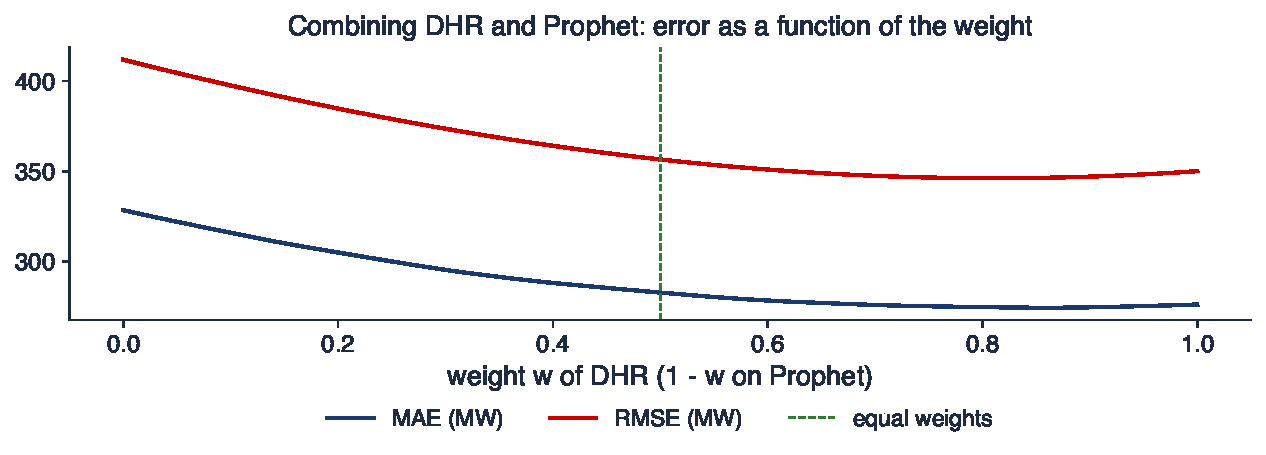
\includegraphics[width=0.97\textwidth,height=0.52\textheight,keepaspectratio]{tsa_ch4_combination.pdf}
\end{center}
\vspace{-0.25cm}
\begin{itemize}
    \item Cross-validation errors of the daily load; $w$ is the weight of DHR
\end{itemize}
\quantlet{TSA\_ch4\_evaluation}{\qlurl{TSA_ch4_evaluation}}
\end{frame}

\begin{frame}{Interpreting the combination}
\itemsize{\footnotesize}
\begin{itemize}
    \item MAE: Prophet alone (w = 0) 328 MW, DHR alone (w = 1) 276 MW, equal weights 283 MW
    \begin{itemize}
        \item best in hindsight: $w = 0.86$, MAE 274 MW, a small gain chosen after seeing the test data
    \end{itemize}
    \item The errors of the two methods are strongly correlated ($\rho = 0.75$): both miss the same cold spells
    \item The five-model average (MAE 305) is second only to DHR and better than four of its five members: cheap insurance when the winner is not known in advance
    \item In the M4 competition (\refMFour), most of the best methods were combinations; review: \refWangComb
\end{itemize}
\end{frame}


%=============================================================================
\section{Possible contribution of AI}
%=============================================================================

\begin{frame}{Possible contribution of AI}
\itemsize{\small}
\begin{itemize}
    \item \textbf{Code}: a first draft of a rolling-origin loop that refits SARIMA, DHR, TBATS and Prophet and stores the errors by horizon
    \item \textbf{Calendars}: lists of holidays and moving feasts for other countries, to be checked against official sources
    \item \textbf{Explanation}: a second derivation of the ACF of the airline model, or of the eventual forecast function
    \item Example prompt
    \begin{itemize}
        \item \aiprompt{Write Python code that forecasts daily electricity load 14 days ahead with a regression on annual Fourier terms, weekday dummies and Romanian public holidays (Orthodox Easter from dateutil) with ARMA errors, and evaluates it against SARIMA by rolling origins and a Diebold-Mariano test.}
    \end{itemize}
\end{itemize}
\end{frame}

\begin{frame}{Checks you must run}
\itemsize{\small}
\begin{itemize}
    \item The Easter date: Orthodox, not Western (\texttt{EASTER\_ORTHODOX}); in 2024 the two differ by five weeks
    \item No look-ahead: features, model orders and holiday lists must be available at each origin
    \item The sign conventions of $\theta$ and $\Theta$ in the software, and the degrees of freedom of Ljung--Box
    \item Adjusted or unadjusted data: SARIMA on NSA; growth rates on the right version
    \item That the DM test uses losses from the same windows for both methods, and the HLN correction for small $n$
    \item Every cited reference: it must exist; check the DOI
\end{itemize}
\end{frame}


%=============================================================================
\section{Summary}
%=============================================================================

\begin{frame}{Key takeaways}
\itemsize{\small}
\begin{itemize}
    \item Seasonality repeats with a known period; it can be deterministic (dummies, Fourier) or stochastic ($\Delta_s$)
    \item SARIMA multiplies regular and seasonal polynomials; the airline model fits many series with two parameters
    \item Official data: SCA for short-run growth, NSA with calendar regressors for SARIMA forecasting
    \item Calendar effects (working days, Orthodox Easter, holidays) are known in advance and often matter more than the model class
    \item Multiple seasonality: MSTL, DHR, TBATS, Prophet; on Romanian daily load, DHR wins out of sample
    \item Judge forecasts by rolling origins, MASE and the DM test; combine them when the winner is uncertain
\end{itemize}
\end{frame}

\begin{frame}{Key formulas}
\itemsize{\small}
{\renewcommand{\arraystretch}{1.35}\begin{center}
\scriptsize
\begin{tabular}{ll}
\toprule
\textbf{Quantity} & \textbf{Formula} \\
\midrule
Seasonal difference & $\Delta_sy_t = (1 - L^s)y_t$, \quad $\Delta\Delta_s = 1 - L - L^s + L^{s+1}$ \\
SARIMA & $\phi(L)\Phi(L^s)(1 - L)^d(1 - L^s)^Dy_t = \theta(L)\Theta(L^s)\varepsilon_t$ \\
Airline & $\rho_1 = \frac{\theta}{1 + \theta^2}$, \quad $\rho_s = \frac{\Theta}{1 + \Theta^2}$, \quad $\rho_{s \pm 1} = \rho_1\rho_s$ \\
Fourier & $\sum_{k=1}^{K}[\alpha_k\sin(2\pi kt/m) + \beta_k\cos(2\pi kt/m)]$ \\
Prophet & $y(t) = g(t) + s(t) + h(t) + \varepsilon_t$ \\
MASE & $\frac1h\sum|e_{T+j}| \,/\, \frac{1}{T - m}\sum|y_t - y_{t-m}|$ \\
DM & $\bar d/\sqrt{\hat V/n}$, \quad $d_t = L(e_{1t}) - L(e_{2t})$ \\
Combination & $w^* = \frac{\sigma_2^2 - \rho\sigma_1\sigma_2}{\sigma_1^2 + \sigma_2^2 - 2\rho\sigma_1\sigma_2}$ \\
\bottomrule
\end{tabular}
\end{center}
}
\end{frame}

\begin{frame}{Self-assessment}
\itemsize{\footnotesize}
\begin{itemize}
    \item \textbf{Question}: how many parameters does SARIMA$(1,1,1)(0,1,1)_{12}$ have, and at which lags does $\varepsilon$ appear?
    \begin{itemize}
        \item \textbf{Answer}: $\phi, \theta, \Theta, \sigma^2$, four; $\varepsilon$ at lags 0, 1, 12, 13 (the last with coefficient $\theta\Theta$)
    \end{itemize}
    \item \textbf{Question}: unadjusted GDP falls by 40\% from Q4 to Q1. Is this a recession?
    \begin{itemize}
        \item \textbf{Answer}: no; it is the seasonal pattern; look at the SCA series or at year-on-year growth
    \end{itemize}
    \item \textbf{Question}: a DM test with 26 windows gives HLN $= -1.93$. Is the first forecast significantly better at 5\%?
    \begin{itemize}
        \item \textbf{Answer}: no: $|-1.93| < t_{0.975}(25) = 2.06$; it is better on average, but not significantly
    \end{itemize}
    \item \textbf{Project idea}: forecast Romanian hourly electricity load with a DHR (daily, weekly and annual Fourier terms, holidays, temperature) against TBATS, Prophet and a combination, by rolling origins and DM tests
    \begin{itemize}
        \item Next: \tsachlink{https://danpele.github.io/Time-Series-Analysis/EN/Courses/chapter5_conditional_volatility_garch.pdf}{Chapter 5}, conditional volatility: ARCH and GARCH models
    \end{itemize}
\end{itemize}
\end{frame}


%=============================================================================
\section{References}
%=============================================================================

\begin{frame}{References (1/2)}
\itemsize{\tiny}
\begin{itemize}
    \item Bandara, K., Hyndman, R. J., \& Bergmeir, C. (2025). MSTL: A seasonal-trend decomposition algorithm for time series with multiple seasonal patterns. \textit{International Journal of Operational Research}, 52(1), 79--98. \href{https://doi.org/10.1504/ijor.2025.143957}{doi:10.1504/ijor.2025.143957}
    \item Bates, J. M., \& Granger, C. W. J. (1969). The combination of forecasts. \textit{Journal of the Operational Research Society}, 20(4), 451--468. \href{https://doi.org/10.1057/jors.1969.103}{doi:10.1057/jors.1969.103}
    \item Bergmeir, C., Hyndman, R. J., \& Koo, B. (2018). A note on the validity of cross-validation for evaluating autoregressive time series prediction. \textit{Computational Statistics \& Data Analysis}, 120, 70--83. \href{https://doi.org/10.1016/j.csda.2017.11.003}{doi:10.1016/j.csda.2017.11.003}
    \item Box, G. E. P., \& Cox, D. R. (1964). An analysis of transformations. \textit{Journal of the Royal Statistical Society, Series B}, 26(2), 211--243. \href{https://doi.org/10.1111/j.2517-6161.1964.tb00553.x}{doi:10.1111/j.2517-6161.1964.tb00553.x}
    \item Box, G. E. P., Jenkins, G. M., \& Reinsel, G. C. (2008). \textit{Time Series Analysis: Forecasting and Control} (4th ed.). Wiley. \href{https://doi.org/10.1002/9781118619193}{doi:10.1002/9781118619193}
    \item Brockwell, P. J., \& Davis, R. A. (2016). \textit{Introduction to Time Series and Forecasting} (3rd ed.). Springer. \href{https://doi.org/10.1007/978-3-319-29854-2}{doi:10.1007/978-3-319-29854-2}
    \item Canova, F., \& Hansen, B. E. (1995). Are seasonal patterns constant over time? A test for seasonal stability. \textit{Journal of Business \& Economic Statistics}, 13(3), 237--252. \href{https://doi.org/10.1080/07350015.1995.10524598}{doi:10.1080/07350015.1995.10524598}
    \item Dagum, E. B., \& Bianconcini, S. (2016). \textit{Seasonal Adjustment Methods and Real Time Trend-Cycle Estimation}. Springer. \href{https://doi.org/10.1007/978-3-319-31822-6}{doi:10.1007/978-3-319-31822-6}
    \item De Livera, A. M., Hyndman, R. J., \& Snyder, R. D. (2011). Forecasting time series with complex seasonal patterns using exponential smoothing. \textit{Journal of the American Statistical Association}, 106(496), 1513--1527. \href{https://doi.org/10.1198/jasa.2011.tm09771}{doi:10.1198/jasa.2011.tm09771}
    \item Diebold, F. X., \& Mariano, R. S. (1995). Comparing predictive accuracy. \textit{Journal of Business \& Economic Statistics}, 13(3), 253--263. \href{https://doi.org/10.1080/07350015.1995.10524599}{doi:10.1080/07350015.1995.10524599}
    \item Eurostat (2024). \textit{ESS Guidelines on Seasonal Adjustment, 2024 edition}. Publications Office of the European Union. \href{https://ec.europa.eu/eurostat/web/products-manuals-and-guidelines/w/ks-gq-24-012}{ec.europa.eu/eurostat}
    \item Findley, D. F., Monsell, B. C., Bell, W. R., Otto, M. C., \& Chen, B.-C. (1998). New capabilities and methods of the X-12-ARIMA seasonal-adjustment program. \textit{Journal of Business \& Economic Statistics}, 16(2), 127--152. \href{https://doi.org/10.1080/07350015.1998.10524743}{doi:10.1080/07350015.1998.10524743}
    \item Harvey, D., Leybourne, S., \& Newbold, P. (1997). Testing the equality of prediction mean squared errors. \textit{International Journal of Forecasting}, 13(2), 281--291. \href{https://doi.org/10.1016/S0169-2070(96)00719-4}{doi:10.1016/S0169-2070(96)00719-4}
    \item Hong, T., Pinson, P., Fan, S., Zareipour, H., Troccoli, A., \& Hyndman, R. J. (2016). Probabilistic energy forecasting: Global Energy Forecasting Competition 2014 and beyond. \textit{International Journal of Forecasting}, 32(3), 896--913. \href{https://doi.org/10.1016/j.ijforecast.2016.02.001}{doi:10.1016/j.ijforecast.2016.02.001}
    \item Huang, C., \& Petukhina, A. (2022). \textit{Applied Time Series Analysis and Forecasting with Python}. Springer. \href{https://doi.org/10.1007/978-3-031-13584-2}{doi:10.1007/978-3-031-13584-2}
    \item Hylleberg, S., Engle, R. F., Granger, C. W. J., \& Yoo, B. S. (1990). Seasonal integration and cointegration. \textit{Journal of Econometrics}, 44(1--2), 215--238. \href{https://doi.org/10.1016/0304-4076(90)90080-D}{doi:10.1016/0304-4076(90)90080-D}
\end{itemize}
\end{frame}

\begin{frame}{References (2/2)}
\itemsize{\tiny}
\begin{itemize}
    \item Hyndman, R. J., \& Athanasopoulos, G. (2021). \textit{Forecasting: Principles and Practice} (3rd ed.). OTexts. \href{https://otexts.com/fpp3/}{otexts.com/fpp3}
    \item Hyndman, R. J., \& Khandakar, Y. (2008). Automatic time series forecasting: The forecast package for R. \textit{Journal of Statistical Software}, 27(3), 1--22. \href{https://doi.org/10.18637/jss.v027.i03}{doi:10.18637/jss.v027.i03}
    \item Hyndman, R. J., \& Koehler, A. B. (2006). Another look at measures of forecast accuracy. \textit{International Journal of Forecasting}, 22(4), 679--688. \href{https://doi.org/10.1016/j.ijforecast.2006.03.001}{doi:10.1016/j.ijforecast.2006.03.001}
    \item Ladiray, D., \& Quenneville, B. (2001). \textit{Seasonal Adjustment with the X-11 Method}. Lecture Notes in Statistics 158. Springer. \href{https://doi.org/10.1007/978-1-4613-0175-2}{doi:10.1007/978-1-4613-0175-2}
    \item Ljung, G. M., \& Box, G. E. P. (1978). On a measure of lack of fit in time series models. \textit{Biometrika}, 65(2), 297--303. \href{https://doi.org/10.1093/biomet/65.2.297}{doi:10.1093/biomet/65.2.297}
    \item Makridakis, S., Spiliotis, E., \& Assimakopoulos, V. (2020). The M4 Competition: 100,000 time series and 61 forecasting methods. \textit{International Journal of Forecasting}, 36(1), 54--74. \href{https://doi.org/10.1016/j.ijforecast.2019.04.014}{doi:10.1016/j.ijforecast.2019.04.014}
    \item Osborn, D. R., Chui, A. P. L., Smith, J. P., \& Birchenhall, C. R. (1988). Seasonality and the order of integration for consumption. \textit{Oxford Bulletin of Economics and Statistics}, 50(4), 361--377. \href{https://doi.org/10.1111/j.1468-0084.1988.mp50004002.x}{doi:10.1111/j.1468-0084.1988.mp50004002.x}
    \item Petropoulos, F., et al. (2022). Forecasting: theory and practice. \textit{International Journal of Forecasting}, 38(3), 705--871. \href{https://doi.org/10.1016/j.ijforecast.2021.11.001}{doi:10.1016/j.ijforecast.2021.11.001}
    \item Smith, J., \& Wallis, K. F. (2009). A simple explanation of the forecast combination puzzle. \textit{Oxford Bulletin of Economics and Statistics}, 71(3), 331--355. \href{https://doi.org/10.1111/j.1468-0084.2008.00541.x}{doi:10.1111/j.1468-0084.2008.00541.x}
    \item Stock, J. H., \& Watson, M. W. (2004). Combination forecasts of output growth in a seven-country data set. \textit{Journal of Forecasting}, 23(6), 405--430. \href{https://doi.org/10.1002/for.928}{doi:10.1002/for.928}
    \item Tashman, L. J. (2000). Out-of-sample tests of forecasting accuracy: an analysis and review. \textit{International Journal of Forecasting}, 16(4), 437--450. \href{https://doi.org/10.1016/S0169-2070(00)00065-0}{doi:10.1016/S0169-2070(00)00065-0}
    \item Taylor, S. J., \& Letham, B. (2018). Forecasting at scale. \textit{The American Statistician}, 72(1), 37--45. \href{https://doi.org/10.1080/00031305.2017.1380080}{doi:10.1080/00031305.2017.1380080}
    \item Wang, X., Hyndman, R. J., Li, F., \& Kang, Y. (2023). Forecast combinations: An over 50-year review. \textit{International Journal of Forecasting}, 39(4), 1518--1547. \href{https://doi.org/10.1016/j.ijforecast.2022.11.005}{doi:10.1016/j.ijforecast.2022.11.005}
\end{itemize}
\end{frame}

\end{document}
